\documentclass[twoside]{book}

% Packages required by doxygen
\usepackage{calc}
\usepackage{doxygen}
\usepackage{graphicx}
\usepackage[utf8]{inputenc}
\usepackage{makeidx}
\usepackage{multicol}
\usepackage{multirow}
\usepackage{textcomp}
\usepackage[table]{xcolor}

% Font selection
\usepackage[T1]{fontenc}
\usepackage{mathptmx}
\usepackage[scaled=.90]{helvet}
\usepackage{courier}
\usepackage{amssymb}
\usepackage{sectsty}
\renewcommand{\familydefault}{\sfdefault}
\allsectionsfont{%
  \fontseries{bc}\selectfont%
  \color{darkgray}%
}
\renewcommand{\DoxyLabelFont}{%
  \fontseries{bc}\selectfont%
  \color{darkgray}%
}

% Page & text layout
\usepackage{geometry}
\geometry{%
  a4paper,%
  top=2.5cm,%
  bottom=2.5cm,%
  left=2.5cm,%
  right=2.5cm%
}
\tolerance=750
\hfuzz=15pt
\hbadness=750
\setlength{\emergencystretch}{15pt}
\setlength{\parindent}{0cm}
\setlength{\parskip}{0.2cm}
\makeatletter
\renewcommand{\paragraph}{%
  \@startsection{paragraph}{4}{0ex}{-1.0ex}{1.0ex}{%
    \normalfont\normalsize\bfseries\SS@parafont%
  }%
}
\renewcommand{\subparagraph}{%
  \@startsection{subparagraph}{5}{0ex}{-1.0ex}{1.0ex}{%
    \normalfont\normalsize\bfseries\SS@subparafont%
  }%
}
\makeatother

% Headers & footers
\usepackage{fancyhdr}
\pagestyle{fancyplain}
\fancyhead[LE]{\fancyplain{}{\bfseries\thepage}}
\fancyhead[CE]{\fancyplain{}{}}
\fancyhead[RE]{\fancyplain{}{\bfseries\leftmark}}
\fancyhead[LO]{\fancyplain{}{\bfseries\rightmark}}
\fancyhead[CO]{\fancyplain{}{}}
\fancyhead[RO]{\fancyplain{}{\bfseries\thepage}}
\fancyfoot[LE]{\fancyplain{}{}}
\fancyfoot[CE]{\fancyplain{}{}}
\fancyfoot[RE]{\fancyplain{}{\bfseries\scriptsize Generated on Mon Sep 22 2014 15\-:53\-:13 for E\-M\-P\-I\-R\-E D\-A by Doxygen }}
\fancyfoot[LO]{\fancyplain{}{\bfseries\scriptsize Generated on Mon Sep 22 2014 15\-:53\-:13 for E\-M\-P\-I\-R\-E D\-A by Doxygen }}
\fancyfoot[CO]{\fancyplain{}{}}
\fancyfoot[RO]{\fancyplain{}{}}
\renewcommand{\footrulewidth}{0.4pt}
\renewcommand{\chaptermark}[1]{%
  \markboth{#1}{}%
}
\renewcommand{\sectionmark}[1]{%
  \markright{\thesection\ #1}%
}

% Indices & bibliography
\usepackage{natbib}
\usepackage[titles]{tocloft}
\setcounter{tocdepth}{3}
\setcounter{secnumdepth}{5}
\makeindex

% Hyperlinks (required, but should be loaded last)
\usepackage{ifpdf}
\ifpdf
  \usepackage[pdftex,pagebackref=true]{hyperref}
\else
  \usepackage[ps2pdf,pagebackref=true]{hyperref}
\fi
\hypersetup{%
  colorlinks=true,%
  linkcolor=blue,%
  citecolor=blue,%
  unicode%
}

% Custom commands
\newcommand{\clearemptydoublepage}{%
  \newpage{\pagestyle{empty}\cleardoublepage}%
}


%===== C O N T E N T S =====

\begin{document}

% Titlepage & ToC
\hypersetup{pageanchor=false}
\pagenumbering{roman}
\begin{titlepage}
\vspace*{7cm}
\begin{center}%
{\Large E\-M\-P\-I\-R\-E D\-A \\[1ex]\large 0.\-1 }\\
\vspace*{1cm}
{\large Generated by Doxygen 1.8.6}\\
\vspace*{0.5cm}
{\small Mon Sep 22 2014 15:53:13}\\
\end{center}
\end{titlepage}
\clearemptydoublepage
\tableofcontents
\clearemptydoublepage
\pagenumbering{arabic}
\hypersetup{pageanchor=true}

%--- Begin generated contents ---
\chapter{Main Page}
\label{index}\hypertarget{index}{}This is where we put the stuff to go at the top of the documentation. looks like this 
\chapter{Data Type Index}
\section{Data Types List}
Here are the data types with brief descriptions\-:\begin{DoxyCompactList}
\item\contentsline{section}{\hyperlink{classcomms}{comms} \\*Module containing E\-M\-P\-I\-R\-E coupling data }{\pageref{classcomms}}{}
\item\contentsline{section}{\hyperlink{classhistogram__data}{histogram\-\_\-data} \\*Module to control what variables are used to generate rank histograms }{\pageref{classhistogram__data}}{}
\item\contentsline{section}{\hyperlink{classhqht__plus__r}{hqht\-\_\-plus\-\_\-r} }{\pageref{classhqht__plus__r}}{}
\item\contentsline{section}{\hyperlink{classpf__control}{pf\-\_\-control} \\*Module to hold all the information to control the the main program }{\pageref{classpf__control}}{}
\item\contentsline{section}{\hyperlink{structpf__control_1_1pf__control__type}{pf\-\_\-control\-::pf\-\_\-control\-\_\-type} }{\pageref{structpf__control_1_1pf__control__type}}{}
\item\contentsline{section}{\hyperlink{classqdata}{qdata} \\*Module as a place to store user specified data for $Q$ }{\pageref{classqdata}}{}
\item\contentsline{section}{\hyperlink{classrandom}{random} \\*A module for random number generation from the following distributions\-: }{\pageref{classrandom}}{}
\item\contentsline{section}{\hyperlink{classrdata}{rdata} \\*Module to hold user supplied data for $R$ observation error covariance matrix }{\pageref{classrdata}}{}
\item\contentsline{section}{\hyperlink{classsizes}{sizes} \\*Module that stores the dimension of observation and state spaces }{\pageref{classsizes}}{}
\end{DoxyCompactList}

\chapter{File Index}
\section{File List}
Here is a list of all files with brief descriptions\-:\begin{DoxyCompactList}
\item\contentsline{section}{src/controlers/\hyperlink{old__pf__couple_8f90}{old\-\_\-pf\-\_\-couple.\-f90} }{\pageref{old__pf__couple_8f90}}{}
\item\contentsline{section}{src/controlers/\hyperlink{pf__control_8f90}{pf\-\_\-control.\-f90} }{\pageref{pf__control_8f90}}{}
\item\contentsline{section}{src/controlers/\hyperlink{pf__couple_8f90}{pf\-\_\-couple.\-f90} }{\pageref{pf__couple_8f90}}{}
\item\contentsline{section}{src/controlers/\hyperlink{sizes_8f90}{sizes.\-f90} }{\pageref{sizes_8f90}}{}
\item\contentsline{section}{src/data/\hyperlink{_qdata_8f90}{Qdata.\-f90} }{\pageref{_qdata_8f90}}{}
\item\contentsline{section}{src/data/\hyperlink{_rdata_8f90}{Rdata.\-f90} }{\pageref{_rdata_8f90}}{}
\item\contentsline{section}{src/filters/\hyperlink{eakf__analysis_8f90}{eakf\-\_\-analysis.\-f90} }{\pageref{eakf__analysis_8f90}}{}
\item\contentsline{section}{src/filters/\hyperlink{enkf__specific_8f90}{enkf\-\_\-specific.\-f90} }{\pageref{enkf__specific_8f90}}{}
\item\contentsline{section}{src/filters/\hyperlink{equivalent__weights__step_8f90}{equivalent\-\_\-weights\-\_\-step.\-f90} }{\pageref{equivalent__weights__step_8f90}}{}
\item\contentsline{section}{src/filters/\hyperlink{etkf__analysis_8f90}{etkf\-\_\-analysis.\-f90} }{\pageref{etkf__analysis_8f90}}{}
\item\contentsline{section}{src/filters/\hyperlink{proposal__filter_8f90}{proposal\-\_\-filter.\-f90} }{\pageref{proposal__filter_8f90}}{}
\item\contentsline{section}{src/filters/\hyperlink{sir__filter_8f90}{sir\-\_\-filter.\-f90} }{\pageref{sir__filter_8f90}}{}
\item\contentsline{section}{src/filters/\hyperlink{stochastic__model_8f90}{stochastic\-\_\-model.\-f90} }{\pageref{stochastic__model_8f90}}{}
\item\contentsline{section}{src/operations/\hyperlink{gen__rand_8f90}{gen\-\_\-rand.\-f90} }{\pageref{gen__rand_8f90}}{}
\item\contentsline{section}{src/operations/\hyperlink{operator__wrappers_8f90}{operator\-\_\-wrappers.\-f90} }{\pageref{operator__wrappers_8f90}}{}
\item\contentsline{section}{src/operations/\hyperlink{perturb__particle_8f90}{perturb\-\_\-particle.\-f90} }{\pageref{perturb__particle_8f90}}{}
\item\contentsline{section}{src/operations/\hyperlink{resample_8f90}{resample.\-f90} }{\pageref{resample_8f90}}{}
\item\contentsline{section}{src/tests/\hyperlink{alltests_8f90}{alltests.\-f90} }{\pageref{alltests_8f90}}{}
\item\contentsline{section}{src/tests/\hyperlink{test__h_8f90}{test\-\_\-h.\-f90} }{\pageref{test__h_8f90}}{}
\item\contentsline{section}{src/tests/\hyperlink{test__hqhtr_8f90}{test\-\_\-hqhtr.\-f90} }{\pageref{test__hqhtr_8f90}}{}
\item\contentsline{section}{src/tests/\hyperlink{test__q_8f90}{test\-\_\-q.\-f90} }{\pageref{test__q_8f90}}{}
\item\contentsline{section}{src/tests/\hyperlink{test__r_8f90}{test\-\_\-r.\-f90} }{\pageref{test__r_8f90}}{}
\item\contentsline{section}{src/tests/\hyperlink{tests_8f90}{tests.\-f90} }{\pageref{tests_8f90}}{}
\item\contentsline{section}{src/utils/\hyperlink{comms_8f90}{comms.\-f90} }{\pageref{comms_8f90}}{}
\item\contentsline{section}{src/utils/\hyperlink{data__io_8f90}{data\-\_\-io.\-f90} }{\pageref{data__io_8f90}}{}
\item\contentsline{section}{src/utils/\hyperlink{diagnostics_8f90}{diagnostics.\-f90} }{\pageref{diagnostics_8f90}}{}
\item\contentsline{section}{src/utils/\hyperlink{gen_q_8f90}{gen\-Q.\-f90} }{\pageref{gen_q_8f90}}{}
\item\contentsline{section}{src/utils/\hyperlink{histogram_8f90}{histogram.\-f90} }{\pageref{histogram_8f90}}{}
\item\contentsline{section}{src/utils/\hyperlink{quicksort_8f90}{quicksort.\-f90} }{\pageref{quicksort_8f90}}{}
\item\contentsline{section}{src/utils/\hyperlink{random__d_8f90}{random\-\_\-d.\-f90} }{\pageref{random__d_8f90}}{}
\end{DoxyCompactList}

\chapter{Data Type Documentation}
\hypertarget{classcomms}{\section{comms Module Reference}
\label{classcomms}\index{comms@{comms}}
}


Module containing E\-M\-P\-I\-R\-E coupling data.  


\subsection*{Public Member Functions}
\begin{DoxyCompactItemize}
\item 
subroutine \hyperlink{classcomms_a61882a03f2b5466163433dd5a3e9e70a}{allocate\-\_\-data}
\item 
subroutine \hyperlink{classcomms_a8841f5445320e65d24a508fa42f10663}{deallocate\-\_\-data}
\item 
subroutine \hyperlink{classcomms_abb286c62a1743d0da16dc3f0495eb501}{initialise\-\_\-mpi}
\begin{DoxyCompactList}\small\item\em subroutine to make E\-M\-P\-I\-R\-E connections and saves details into \hyperlink{classpf__control}{pf\-\_\-control} module \end{DoxyCompactList}\end{DoxyCompactItemize}
\subsection*{Public Attributes}
\begin{DoxyCompactItemize}
\item 
integer \hyperlink{classcomms_a9a38af536275f02674f67d814566ef67}{cpl\-\_\-mpi\-\_\-comm}
\item 
integer \hyperlink{classcomms_adcd9567cc8bd6f78dc184ff3bd433eb8}{mype\-\_\-id}
\item 
integer \hyperlink{classcomms_a0dead85d30852fd43b3667663c98695c}{myrank}
\item 
integer \hyperlink{classcomms_a4d6c1b5d6aa807f60683ccf2cdb89644}{nproc}
\item 
integer \hyperlink{classcomms_a86ca20605ce853814b00dd91fdd0db89}{pf\-\_\-mpi\-\_\-comm}
\item 
integer \hyperlink{classcomms_ac714c7b76943c8057f54dc27bd5575fb}{pfrank}
\item 
integer \hyperlink{classcomms_a0120cad068b402a882222d566d18790e}{npfs}
\item 
integer, dimension(\-:), allocatable \hyperlink{classcomms_a4912d43983e564849625e5588af33348}{gblcount}
\item 
integer, dimension(\-:), allocatable \hyperlink{classcomms_a7b71c5edbea32c7dae3333cb1c05f3fe}{gbldisp}
\end{DoxyCompactItemize}


\subsection{Detailed Description}
Module containing E\-M\-P\-I\-R\-E coupling data. 

\subsection{Member Function/\-Subroutine Documentation}
\hypertarget{classcomms_a61882a03f2b5466163433dd5a3e9e70a}{\index{comms@{comms}!allocate\-\_\-data@{allocate\-\_\-data}}
\index{allocate\-\_\-data@{allocate\-\_\-data}!comms@{comms}}
\subsubsection[{allocate\-\_\-data}]{\setlength{\rightskip}{0pt plus 5cm}subroutine comms\-::allocate\-\_\-data (
\begin{DoxyParamCaption}
{}
\end{DoxyParamCaption}
)}}\label{classcomms_a61882a03f2b5466163433dd5a3e9e70a}
\hypertarget{classcomms_a8841f5445320e65d24a508fa42f10663}{\index{comms@{comms}!deallocate\-\_\-data@{deallocate\-\_\-data}}
\index{deallocate\-\_\-data@{deallocate\-\_\-data}!comms@{comms}}
\subsubsection[{deallocate\-\_\-data}]{\setlength{\rightskip}{0pt plus 5cm}subroutine comms\-::deallocate\-\_\-data (
\begin{DoxyParamCaption}
{}
\end{DoxyParamCaption}
)}}\label{classcomms_a8841f5445320e65d24a508fa42f10663}


Here is the caller graph for this function\-:\nopagebreak
\begin{figure}[H]
\begin{center}
\leavevmode
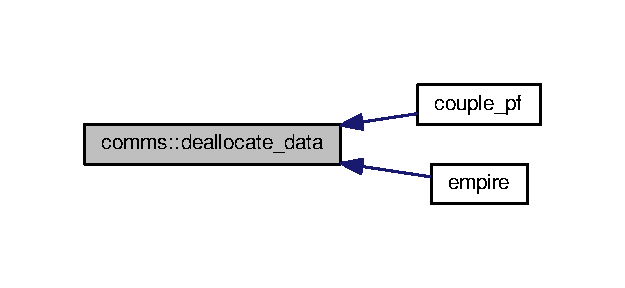
\includegraphics[width=300pt]{classcomms_a8841f5445320e65d24a508fa42f10663_icgraph}
\end{center}
\end{figure}


\hypertarget{classcomms_abb286c62a1743d0da16dc3f0495eb501}{\index{comms@{comms}!initialise\-\_\-mpi@{initialise\-\_\-mpi}}
\index{initialise\-\_\-mpi@{initialise\-\_\-mpi}!comms@{comms}}
\subsubsection[{initialise\-\_\-mpi}]{\setlength{\rightskip}{0pt plus 5cm}subroutine comms\-::initialise\-\_\-mpi (
\begin{DoxyParamCaption}
{}
\end{DoxyParamCaption}
)}}\label{classcomms_abb286c62a1743d0da16dc3f0495eb501}


subroutine to make E\-M\-P\-I\-R\-E connections and saves details into \hyperlink{classpf__control}{pf\-\_\-control} module 



Here is the caller graph for this function\-:\nopagebreak
\begin{figure}[H]
\begin{center}
\leavevmode
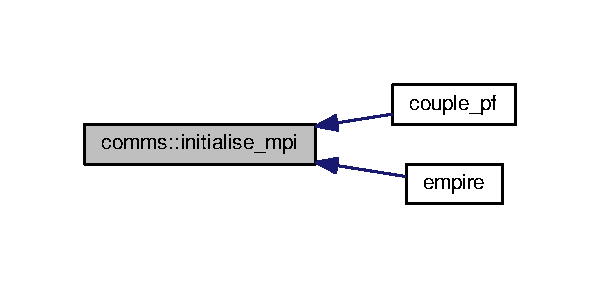
\includegraphics[width=288pt]{classcomms_abb286c62a1743d0da16dc3f0495eb501_icgraph}
\end{center}
\end{figure}




\subsection{Member Data Documentation}
\hypertarget{classcomms_a9a38af536275f02674f67d814566ef67}{\index{comms@{comms}!cpl\-\_\-mpi\-\_\-comm@{cpl\-\_\-mpi\-\_\-comm}}
\index{cpl\-\_\-mpi\-\_\-comm@{cpl\-\_\-mpi\-\_\-comm}!comms@{comms}}
\subsubsection[{cpl\-\_\-mpi\-\_\-comm}]{\setlength{\rightskip}{0pt plus 5cm}integer comms\-::cpl\-\_\-mpi\-\_\-comm}}\label{classcomms_a9a38af536275f02674f67d814566ef67}
\hypertarget{classcomms_a4912d43983e564849625e5588af33348}{\index{comms@{comms}!gblcount@{gblcount}}
\index{gblcount@{gblcount}!comms@{comms}}
\subsubsection[{gblcount}]{\setlength{\rightskip}{0pt plus 5cm}integer, dimension(\-:), allocatable comms\-::gblcount}}\label{classcomms_a4912d43983e564849625e5588af33348}
\hypertarget{classcomms_a7b71c5edbea32c7dae3333cb1c05f3fe}{\index{comms@{comms}!gbldisp@{gbldisp}}
\index{gbldisp@{gbldisp}!comms@{comms}}
\subsubsection[{gbldisp}]{\setlength{\rightskip}{0pt plus 5cm}integer, dimension(\-:), allocatable comms\-::gbldisp}}\label{classcomms_a7b71c5edbea32c7dae3333cb1c05f3fe}
\hypertarget{classcomms_adcd9567cc8bd6f78dc184ff3bd433eb8}{\index{comms@{comms}!mype\-\_\-id@{mype\-\_\-id}}
\index{mype\-\_\-id@{mype\-\_\-id}!comms@{comms}}
\subsubsection[{mype\-\_\-id}]{\setlength{\rightskip}{0pt plus 5cm}integer comms\-::mype\-\_\-id}}\label{classcomms_adcd9567cc8bd6f78dc184ff3bd433eb8}
\hypertarget{classcomms_a0dead85d30852fd43b3667663c98695c}{\index{comms@{comms}!myrank@{myrank}}
\index{myrank@{myrank}!comms@{comms}}
\subsubsection[{myrank}]{\setlength{\rightskip}{0pt plus 5cm}integer comms\-::myrank}}\label{classcomms_a0dead85d30852fd43b3667663c98695c}
\hypertarget{classcomms_a0120cad068b402a882222d566d18790e}{\index{comms@{comms}!npfs@{npfs}}
\index{npfs@{npfs}!comms@{comms}}
\subsubsection[{npfs}]{\setlength{\rightskip}{0pt plus 5cm}integer comms\-::npfs}}\label{classcomms_a0120cad068b402a882222d566d18790e}
\hypertarget{classcomms_a4d6c1b5d6aa807f60683ccf2cdb89644}{\index{comms@{comms}!nproc@{nproc}}
\index{nproc@{nproc}!comms@{comms}}
\subsubsection[{nproc}]{\setlength{\rightskip}{0pt plus 5cm}integer comms\-::nproc}}\label{classcomms_a4d6c1b5d6aa807f60683ccf2cdb89644}
\hypertarget{classcomms_a86ca20605ce853814b00dd91fdd0db89}{\index{comms@{comms}!pf\-\_\-mpi\-\_\-comm@{pf\-\_\-mpi\-\_\-comm}}
\index{pf\-\_\-mpi\-\_\-comm@{pf\-\_\-mpi\-\_\-comm}!comms@{comms}}
\subsubsection[{pf\-\_\-mpi\-\_\-comm}]{\setlength{\rightskip}{0pt plus 5cm}integer comms\-::pf\-\_\-mpi\-\_\-comm}}\label{classcomms_a86ca20605ce853814b00dd91fdd0db89}
\hypertarget{classcomms_ac714c7b76943c8057f54dc27bd5575fb}{\index{comms@{comms}!pfrank@{pfrank}}
\index{pfrank@{pfrank}!comms@{comms}}
\subsubsection[{pfrank}]{\setlength{\rightskip}{0pt plus 5cm}integer comms\-::pfrank}}\label{classcomms_ac714c7b76943c8057f54dc27bd5575fb}


The documentation for this module was generated from the following file\-:\begin{DoxyCompactItemize}
\item 
src/utils/\hyperlink{comms_8f90}{comms.\-f90}\end{DoxyCompactItemize}

\hypertarget{classhistogram__data}{\section{histogram\-\_\-data Module Reference}
\label{classhistogram__data}\index{histogram\-\_\-data@{histogram\-\_\-data}}
}


Module to control what variables are used to generate rank histograms.  


\subsection*{Public Member Functions}
\begin{DoxyCompactItemize}
\item 
subroutine \hyperlink{classhistogram__data_a589a496c989be1af671e85ee0e4eadff}{load\-\_\-histogram\-\_\-data}
\begin{DoxyCompactList}\small\item\em subroutine to read from variables\-\_\-hist.\-dat which variables to be used to make the rank histograms \end{DoxyCompactList}\item 
subroutine \hyperlink{classhistogram__data_acc52068812749b7315e706a2539f101f}{kill\-\_\-histogram\-\_\-data}
\begin{DoxyCompactList}\small\item\em subroutine to clean up arrays used in rank histograms \end{DoxyCompactList}\end{DoxyCompactItemize}
\subsection*{Public Attributes}
\begin{DoxyCompactItemize}
\item 
integer, dimension(\-:), allocatable \hyperlink{classhistogram__data_a2f7cb336d665046859ebe5684ed09be8}{rank\-\_\-hist\-\_\-list}
\item 
integer, dimension(\-:), allocatable \hyperlink{classhistogram__data_a94a5c8fc25a86b8f62b2ff301de78d32}{rank\-\_\-hist\-\_\-nums}
\item 
integer \hyperlink{classhistogram__data_ac202796c6c4bfb9c3a16bd8c4b277eba}{rhl\-\_\-n}
\item 
integer \hyperlink{classhistogram__data_a8ac6a785fa075b9bf4d162e2833635d3}{rhn\-\_\-n}
\end{DoxyCompactItemize}


\subsection{Detailed Description}
Module to control what variables are used to generate rank histograms. 

\subsection{Member Function/\-Subroutine Documentation}
\hypertarget{classhistogram__data_acc52068812749b7315e706a2539f101f}{\index{histogram\-\_\-data@{histogram\-\_\-data}!kill\-\_\-histogram\-\_\-data@{kill\-\_\-histogram\-\_\-data}}
\index{kill\-\_\-histogram\-\_\-data@{kill\-\_\-histogram\-\_\-data}!histogram_data@{histogram\-\_\-data}}
\subsubsection[{kill\-\_\-histogram\-\_\-data}]{\setlength{\rightskip}{0pt plus 5cm}subroutine histogram\-\_\-data\-::kill\-\_\-histogram\-\_\-data (
\begin{DoxyParamCaption}
{}
\end{DoxyParamCaption}
)}}\label{classhistogram__data_acc52068812749b7315e706a2539f101f}


subroutine to clean up arrays used in rank histograms 

\hypertarget{classhistogram__data_a589a496c989be1af671e85ee0e4eadff}{\index{histogram\-\_\-data@{histogram\-\_\-data}!load\-\_\-histogram\-\_\-data@{load\-\_\-histogram\-\_\-data}}
\index{load\-\_\-histogram\-\_\-data@{load\-\_\-histogram\-\_\-data}!histogram_data@{histogram\-\_\-data}}
\subsubsection[{load\-\_\-histogram\-\_\-data}]{\setlength{\rightskip}{0pt plus 5cm}subroutine histogram\-\_\-data\-::load\-\_\-histogram\-\_\-data (
\begin{DoxyParamCaption}
{}
\end{DoxyParamCaption}
)}}\label{classhistogram__data_a589a496c989be1af671e85ee0e4eadff}


subroutine to read from variables\-\_\-hist.\-dat which variables to be used to make the rank histograms 



\subsection{Member Data Documentation}
\hypertarget{classhistogram__data_a2f7cb336d665046859ebe5684ed09be8}{\index{histogram\-\_\-data@{histogram\-\_\-data}!rank\-\_\-hist\-\_\-list@{rank\-\_\-hist\-\_\-list}}
\index{rank\-\_\-hist\-\_\-list@{rank\-\_\-hist\-\_\-list}!histogram_data@{histogram\-\_\-data}}
\subsubsection[{rank\-\_\-hist\-\_\-list}]{\setlength{\rightskip}{0pt plus 5cm}integer, dimension(\-:), allocatable histogram\-\_\-data\-::rank\-\_\-hist\-\_\-list}}\label{classhistogram__data_a2f7cb336d665046859ebe5684ed09be8}
\hypertarget{classhistogram__data_a94a5c8fc25a86b8f62b2ff301de78d32}{\index{histogram\-\_\-data@{histogram\-\_\-data}!rank\-\_\-hist\-\_\-nums@{rank\-\_\-hist\-\_\-nums}}
\index{rank\-\_\-hist\-\_\-nums@{rank\-\_\-hist\-\_\-nums}!histogram_data@{histogram\-\_\-data}}
\subsubsection[{rank\-\_\-hist\-\_\-nums}]{\setlength{\rightskip}{0pt plus 5cm}integer, dimension(\-:), allocatable histogram\-\_\-data\-::rank\-\_\-hist\-\_\-nums}}\label{classhistogram__data_a94a5c8fc25a86b8f62b2ff301de78d32}
\hypertarget{classhistogram__data_ac202796c6c4bfb9c3a16bd8c4b277eba}{\index{histogram\-\_\-data@{histogram\-\_\-data}!rhl\-\_\-n@{rhl\-\_\-n}}
\index{rhl\-\_\-n@{rhl\-\_\-n}!histogram_data@{histogram\-\_\-data}}
\subsubsection[{rhl\-\_\-n}]{\setlength{\rightskip}{0pt plus 5cm}integer histogram\-\_\-data\-::rhl\-\_\-n}}\label{classhistogram__data_ac202796c6c4bfb9c3a16bd8c4b277eba}
\hypertarget{classhistogram__data_a8ac6a785fa075b9bf4d162e2833635d3}{\index{histogram\-\_\-data@{histogram\-\_\-data}!rhn\-\_\-n@{rhn\-\_\-n}}
\index{rhn\-\_\-n@{rhn\-\_\-n}!histogram_data@{histogram\-\_\-data}}
\subsubsection[{rhn\-\_\-n}]{\setlength{\rightskip}{0pt plus 5cm}integer histogram\-\_\-data\-::rhn\-\_\-n}}\label{classhistogram__data_a8ac6a785fa075b9bf4d162e2833635d3}


The documentation for this module was generated from the following file\-:\begin{DoxyCompactItemize}
\item 
src/utils/\hyperlink{histogram_8f90}{histogram.\-f90}\end{DoxyCompactItemize}

\hypertarget{classhqht__plus__r}{\section{hqht\-\_\-plus\-\_\-r Module Reference}
\label{classhqht__plus__r}\index{hqht\-\_\-plus\-\_\-r@{hqht\-\_\-plus\-\_\-r}}
}
\subsection*{Public Member Functions}
\begin{DoxyCompactItemize}
\item 
subroutine \hyperlink{classhqht__plus__r_a7e2c2b1fe5468652a61a0fb00333a116}{load\-\_\-hqhtr}
\item 
subroutine \hyperlink{classhqht__plus__r_a4f932903b26bd25447c37f8358b968da}{hqhtr\-\_\-factor}
\item 
subroutine \hyperlink{classhqht__plus__r_a71503dae1f32552b708ac51e6f7e5d38}{kill\-\_\-hqhtr}
\end{DoxyCompactItemize}


\subsection{Member Function/\-Subroutine Documentation}
\hypertarget{classhqht__plus__r_a4f932903b26bd25447c37f8358b968da}{\index{hqht\-\_\-plus\-\_\-r@{hqht\-\_\-plus\-\_\-r}!hqhtr\-\_\-factor@{hqhtr\-\_\-factor}}
\index{hqhtr\-\_\-factor@{hqhtr\-\_\-factor}!hqht_plus_r@{hqht\-\_\-plus\-\_\-r}}
\subsubsection[{hqhtr\-\_\-factor}]{\setlength{\rightskip}{0pt plus 5cm}subroutine hqht\-\_\-plus\-\_\-r\-::hqhtr\-\_\-factor (
\begin{DoxyParamCaption}
{}
\end{DoxyParamCaption}
)}}\label{classhqht__plus__r_a4f932903b26bd25447c37f8358b968da}


Here is the caller graph for this function\-:\nopagebreak
\begin{figure}[H]
\begin{center}
\leavevmode
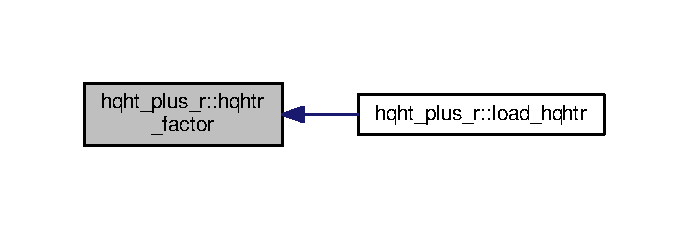
\includegraphics[width=330pt]{classhqht__plus__r_a4f932903b26bd25447c37f8358b968da_icgraph}
\end{center}
\end{figure}


\hypertarget{classhqht__plus__r_a71503dae1f32552b708ac51e6f7e5d38}{\index{hqht\-\_\-plus\-\_\-r@{hqht\-\_\-plus\-\_\-r}!kill\-\_\-hqhtr@{kill\-\_\-hqhtr}}
\index{kill\-\_\-hqhtr@{kill\-\_\-hqhtr}!hqht_plus_r@{hqht\-\_\-plus\-\_\-r}}
\subsubsection[{kill\-\_\-hqhtr}]{\setlength{\rightskip}{0pt plus 5cm}subroutine hqht\-\_\-plus\-\_\-r\-::kill\-\_\-hqhtr (
\begin{DoxyParamCaption}
{}
\end{DoxyParamCaption}
)}}\label{classhqht__plus__r_a71503dae1f32552b708ac51e6f7e5d38}
\hypertarget{classhqht__plus__r_a7e2c2b1fe5468652a61a0fb00333a116}{\index{hqht\-\_\-plus\-\_\-r@{hqht\-\_\-plus\-\_\-r}!load\-\_\-hqhtr@{load\-\_\-hqhtr}}
\index{load\-\_\-hqhtr@{load\-\_\-hqhtr}!hqht_plus_r@{hqht\-\_\-plus\-\_\-r}}
\subsubsection[{load\-\_\-hqhtr}]{\setlength{\rightskip}{0pt plus 5cm}subroutine hqht\-\_\-plus\-\_\-r\-::load\-\_\-hqhtr (
\begin{DoxyParamCaption}
{}
\end{DoxyParamCaption}
)}}\label{classhqht__plus__r_a7e2c2b1fe5468652a61a0fb00333a116}


Here is the call graph for this function\-:\nopagebreak
\begin{figure}[H]
\begin{center}
\leavevmode
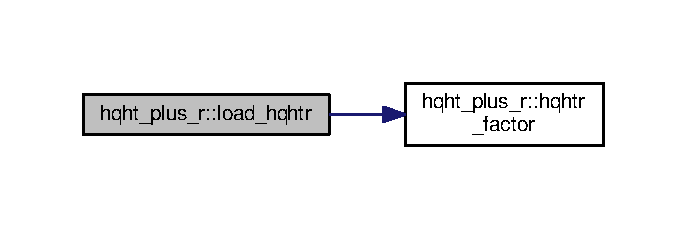
\includegraphics[width=330pt]{classhqht__plus__r_a7e2c2b1fe5468652a61a0fb00333a116_cgraph}
\end{center}
\end{figure}




The documentation for this module was generated from the following file\-:\begin{DoxyCompactItemize}
\item 
src/data/\hyperlink{_rdata_8f90}{Rdata.\-f90}\end{DoxyCompactItemize}

\hypertarget{classpf__control}{\section{pf\-\_\-control Module Reference}
\label{classpf__control}\index{pf\-\_\-control@{pf\-\_\-control}}
}


module to hold all the information to control the the main program  




Collaboration diagram for pf\-\_\-control\-:\nopagebreak
\begin{figure}[H]
\begin{center}
\leavevmode
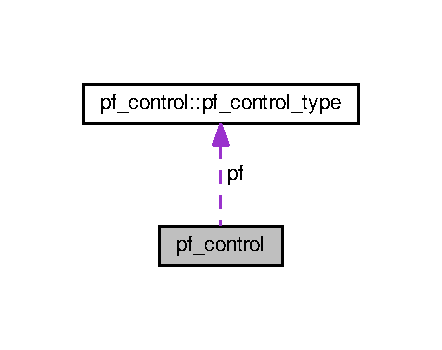
\includegraphics[width=212pt]{classpf__control__coll__graph}
\end{center}
\end{figure}
\subsection*{Data Types}
\begin{DoxyCompactItemize}
\item 
type \hyperlink{structpf__control_1_1pf__control__type}{pf\-\_\-control\-\_\-type}
\end{DoxyCompactItemize}
\subsection*{Public Member Functions}
\begin{DoxyCompactItemize}
\item 
subroutine \hyperlink{classpf__control_a51d23c79a8d8c8990693e6a3c3fd677d}{set\-\_\-pf\-\_\-controls}
\item 
subroutine \hyperlink{classpf__control_ac9178a97a8f6b9e8065f85c3ed790104}{allocate\-\_\-pf}
\item 
subroutine \hyperlink{classpf__control_a27e74873fa25af0939a3f824954857f4}{deallocate\-\_\-pf}
\end{DoxyCompactItemize}
\subsection*{Public Attributes}
\begin{DoxyCompactItemize}
\item 
type(\hyperlink{structpf__control_1_1pf__control__type}{pf\-\_\-control\-\_\-type}) \hyperlink{classpf__control_aa7bb53e2dfc844fb482e69ac9b483415}{pf}
\begin{DoxyCompactList}\small\item\em the derived data type holding all controlling data \end{DoxyCompactList}\end{DoxyCompactItemize}


\subsection{Detailed Description}
module to hold all the information to control the the main program 

\subsection{Member Function/\-Subroutine Documentation}
\hypertarget{classpf__control_ac9178a97a8f6b9e8065f85c3ed790104}{\index{pf\-\_\-control@{pf\-\_\-control}!allocate\-\_\-pf@{allocate\-\_\-pf}}
\index{allocate\-\_\-pf@{allocate\-\_\-pf}!pf_control@{pf\-\_\-control}}
\subsubsection[{allocate\-\_\-pf}]{\setlength{\rightskip}{0pt plus 5cm}subroutine pf\-\_\-control\-::allocate\-\_\-pf (
\begin{DoxyParamCaption}
{}
\end{DoxyParamCaption}
)}}\label{classpf__control_ac9178a97a8f6b9e8065f85c3ed790104}


Here is the caller graph for this function\-:\nopagebreak
\begin{figure}[H]
\begin{center}
\leavevmode
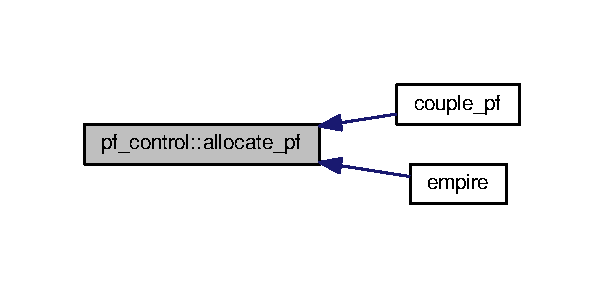
\includegraphics[width=290pt]{classpf__control_ac9178a97a8f6b9e8065f85c3ed790104_icgraph}
\end{center}
\end{figure}


\hypertarget{classpf__control_a27e74873fa25af0939a3f824954857f4}{\index{pf\-\_\-control@{pf\-\_\-control}!deallocate\-\_\-pf@{deallocate\-\_\-pf}}
\index{deallocate\-\_\-pf@{deallocate\-\_\-pf}!pf_control@{pf\-\_\-control}}
\subsubsection[{deallocate\-\_\-pf}]{\setlength{\rightskip}{0pt plus 5cm}subroutine pf\-\_\-control\-::deallocate\-\_\-pf (
\begin{DoxyParamCaption}
{}
\end{DoxyParamCaption}
)}}\label{classpf__control_a27e74873fa25af0939a3f824954857f4}
\hypertarget{classpf__control_a51d23c79a8d8c8990693e6a3c3fd677d}{\index{pf\-\_\-control@{pf\-\_\-control}!set\-\_\-pf\-\_\-controls@{set\-\_\-pf\-\_\-controls}}
\index{set\-\_\-pf\-\_\-controls@{set\-\_\-pf\-\_\-controls}!pf_control@{pf\-\_\-control}}
\subsubsection[{set\-\_\-pf\-\_\-controls}]{\setlength{\rightskip}{0pt plus 5cm}subroutine pf\-\_\-control\-::set\-\_\-pf\-\_\-controls (
\begin{DoxyParamCaption}
{}
\end{DoxyParamCaption}
)}}\label{classpf__control_a51d23c79a8d8c8990693e6a3c3fd677d}


Here is the caller graph for this function\-:\nopagebreak
\begin{figure}[H]
\begin{center}
\leavevmode
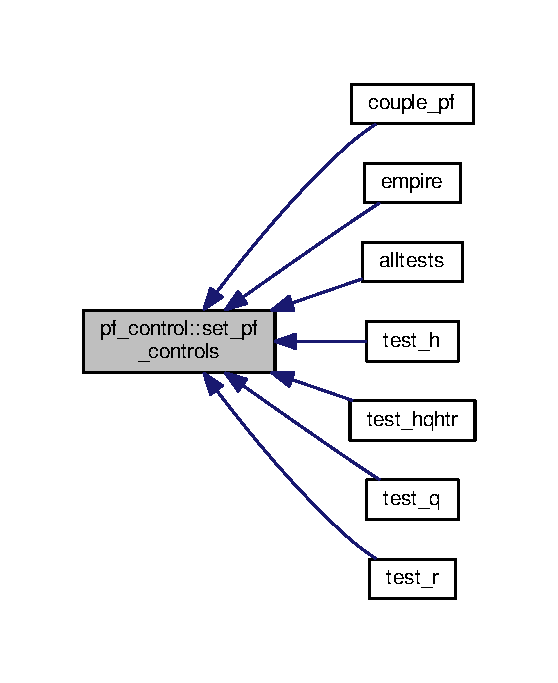
\includegraphics[width=268pt]{classpf__control_a51d23c79a8d8c8990693e6a3c3fd677d_icgraph}
\end{center}
\end{figure}




\subsection{Member Data Documentation}
\hypertarget{classpf__control_aa7bb53e2dfc844fb482e69ac9b483415}{\index{pf\-\_\-control@{pf\-\_\-control}!pf@{pf}}
\index{pf@{pf}!pf_control@{pf\-\_\-control}}
\subsubsection[{pf}]{\setlength{\rightskip}{0pt plus 5cm}type({\bf pf\-\_\-control\-\_\-type}) pf\-\_\-control\-::pf}}\label{classpf__control_aa7bb53e2dfc844fb482e69ac9b483415}


the derived data type holding all controlling data 



The documentation for this module was generated from the following file\-:\begin{DoxyCompactItemize}
\item 
src/controlers/\hyperlink{pf__control_8f90}{pf\-\_\-control.\-f90}\end{DoxyCompactItemize}

\hypertarget{structpf__control_1_1pf__control__type}{\section{pf\-\_\-control\-:\-:pf\-\_\-control\-\_\-type Type Reference}
\label{structpf__control_1_1pf__control__type}\index{pf\-\_\-control\-::pf\-\_\-control\-\_\-type@{pf\-\_\-control\-::pf\-\_\-control\-\_\-type}}
}
\subsection*{Public Attributes}
\begin{DoxyCompactItemize}
\item 
integer \hyperlink{structpf__control_1_1pf__control__type_a54b2dd5d94eb5fd34e0384490b7a293e}{nens}
\begin{DoxyCompactList}\small\item\em the total number of ensemble members \end{DoxyCompactList}\item 
real(kind=kind(1.\-0d0)), dimension(\-:), allocatable \hyperlink{structpf__control_1_1pf__control__type_a6924d4f75cbd9e358263f7cfe453e063}{weight}
\begin{DoxyCompactList}\small\item\em the negative log of the weights of the particles \end{DoxyCompactList}\item 
integer \hyperlink{structpf__control_1_1pf__control__type_a7199be1c1a99f9f066af0ee214f51824}{time\-\_\-obs}
\begin{DoxyCompactList}\small\item\em the number of observations we will assimilate \end{DoxyCompactList}\item 
integer \hyperlink{structpf__control_1_1pf__control__type_a13e65bce20eb3de30403efca169f9635}{time\-\_\-bwn\-\_\-obs}
\begin{DoxyCompactList}\small\item\em the number of model timesteps between observations \end{DoxyCompactList}\item 
real(kind=kind(1.\-0d0)) \hyperlink{structpf__control_1_1pf__control__type_ae8e8786c073ded3dc39645629863cb73}{nudgefac}
\begin{DoxyCompactList}\small\item\em the nudging factor \end{DoxyCompactList}\item 
logical \hyperlink{structpf__control_1_1pf__control__type_a250ef33de2e01234ed341b9864338b7d}{gen\-\_\-data}
\begin{DoxyCompactList}\small\item\em true generates synthetic obs for a twin experiment \end{DoxyCompactList}\item 
logical \hyperlink{structpf__control_1_1pf__control__type_ae1e2616b063090ccd403e0f1c7820fce}{gen\-\_\-q}
\begin{DoxyCompactList}\small\item\em true attempts to build up $Q$ from long model run \end{DoxyCompactList}\item 
logical \hyperlink{structpf__control_1_1pf__control__type_a8b7974924f8883cc71d3fd7d3ef66a9b}{human\-\_\-readable}
\begin{DoxyCompactList}\small\item\em unused \end{DoxyCompactList}\item 
integer \hyperlink{structpf__control_1_1pf__control__type_a12beb826016805c71fcc112a733f2330}{timestep} =0
\begin{DoxyCompactList}\small\item\em the current timestep as the model progresses \end{DoxyCompactList}\item 
real(kind=kind(1.\-0d0)), dimension(\-:,\-:), allocatable \hyperlink{structpf__control_1_1pf__control__type_a3e5d92f215b032c3a563de43278c937f}{psi}
\begin{DoxyCompactList}\small\item\em state vector of ensemble members on this mpi process \end{DoxyCompactList}\item 
real(kind=kind(1.\-0d0)), dimension(\-:), allocatable \hyperlink{structpf__control_1_1pf__control__type_a90ea6d211c5b4d70ab99e12e9a8dc8d5}{mean}
\begin{DoxyCompactList}\small\item\em mean state vector \end{DoxyCompactList}\item 
real(kind=kind(1.\-0d0)) \hyperlink{structpf__control_1_1pf__control__type_a77aec7df0491895c8300476fb856b80a}{nfac}
\begin{DoxyCompactList}\small\item\em standard deviation of normal distribution in mixture density \end{DoxyCompactList}\item 
real(kind=kind(1.\-0d0)) \hyperlink{structpf__control_1_1pf__control__type_a41d48f1ac4e0d69dcea1cd99a62fca90}{ufac}
\begin{DoxyCompactList}\small\item\em half width of the uniform distribution in mixture density \end{DoxyCompactList}\item 
real(kind=kind(1.\-0d0)) \hyperlink{structpf__control_1_1pf__control__type_a105254bf19b7d9582f187d6fefe3b8eb}{efac}
\item 
real(kind=kind(1.\-0d0)) \hyperlink{structpf__control_1_1pf__control__type_a32d13f7de6d41376980374e9ae2c2a62}{keep}
\begin{DoxyCompactList}\small\item\em proportion of particles to keep in E\-W\-P\-F E\-W step \end{DoxyCompactList}\item 
real(kind=kind(1.\-0d0)) \hyperlink{structpf__control_1_1pf__control__type_a4240d041987192d6b192b6910efeb29a}{time}
\begin{DoxyCompactList}\small\item\em dunno \end{DoxyCompactList}\item 
real(kind=kind(1.\-0d0)) \hyperlink{structpf__control_1_1pf__control__type_a48fc82562f2982c72312a1bba7d03d0d}{qscale}
\begin{DoxyCompactList}\small\item\em scalar to multiply Q by \end{DoxyCompactList}\item 
integer \hyperlink{structpf__control_1_1pf__control__type_a739b1b0b9ed322b84b834b9a185fe238}{couple\-\_\-root}
\begin{DoxyCompactList}\small\item\em empire master processor \end{DoxyCompactList}\item 
logical \hyperlink{structpf__control_1_1pf__control__type_a8acf4d56e3c012a8d5761ade51cfc48e}{use\-\_\-talagrand}
\begin{DoxyCompactList}\small\item\em switch if true outputs rank histograms \end{DoxyCompactList}\item 
logical \hyperlink{structpf__control_1_1pf__control__type_ac8097ede5f988970340635da9c936264}{use\-\_\-weak}
\begin{DoxyCompactList}\small\item\em switch unused \end{DoxyCompactList}\item 
logical \hyperlink{structpf__control_1_1pf__control__type_a9fb54b12465d1b75e7337fa7b569cac8}{use\-\_\-mean}
\begin{DoxyCompactList}\small\item\em switch if true outputs ensemble mean \end{DoxyCompactList}\item 
logical \hyperlink{structpf__control_1_1pf__control__type_a0ddc8995c902c77e0a04f70f701f3a5b}{use\-\_\-var}
\begin{DoxyCompactList}\small\item\em switch if true outputs ensemble variance \end{DoxyCompactList}\item 
logical \hyperlink{structpf__control_1_1pf__control__type_a6c3195c3fb580a3d68c0b449a5ce6ab1}{use\-\_\-traj}
\begin{DoxyCompactList}\small\item\em switch if true outputs trajectories \end{DoxyCompactList}\item 
logical \hyperlink{structpf__control_1_1pf__control__type_a47eb88fd006d8ac00206cfd20cd41622}{use\-\_\-rmse}
\begin{DoxyCompactList}\small\item\em switch if true outputs Root Mean Square Errors \end{DoxyCompactList}\item 
integer, dimension(\-:,\-:), \\*
allocatable \hyperlink{structpf__control_1_1pf__control__type_aa35adefc9a96845c065fd01ecf99b37d}{talagrand}
\begin{DoxyCompactList}\small\item\em storage for rank histograms \end{DoxyCompactList}\item 
integer \hyperlink{structpf__control_1_1pf__control__type_a8e26d20b11d6b909dc10731cd3e8d42f}{count}
\begin{DoxyCompactList}\small\item\em number of ensemble members associated with this M\-P\-I process \end{DoxyCompactList}\item 
integer, dimension(\-:), allocatable \hyperlink{structpf__control_1_1pf__control__type_a5a15db12bd5e3ab8163049e4412cf755}{particles}
\begin{DoxyCompactList}\small\item\em particles associates with this M\-P\-I process \end{DoxyCompactList}\item 
character(2) \hyperlink{structpf__control_1_1pf__control__type_ab21afb0aa9c7933073356dbc2155870c}{type}
\begin{DoxyCompactList}\small\item\em which filter to use \end{DoxyCompactList}\item 
character(1) \hyperlink{structpf__control_1_1pf__control__type_ab024d9ea51de1956c671b483f1c9d020}{init}
\begin{DoxyCompactList}\small\item\em which method to initialise ensemble \end{DoxyCompactList}\end{DoxyCompactItemize}


\subsection{Member Data Documentation}
\hypertarget{structpf__control_1_1pf__control__type_a8e26d20b11d6b909dc10731cd3e8d42f}{\index{pf\-\_\-control\-::pf\-\_\-control\-\_\-type@{pf\-\_\-control\-::pf\-\_\-control\-\_\-type}!count@{count}}
\index{count@{count}!pf_control::pf_control_type@{pf\-\_\-control\-::pf\-\_\-control\-\_\-type}}
\subsubsection[{count}]{\setlength{\rightskip}{0pt plus 5cm}integer pf\-\_\-control\-::pf\-\_\-control\-\_\-type\-::count}}\label{structpf__control_1_1pf__control__type_a8e26d20b11d6b909dc10731cd3e8d42f}


number of ensemble members associated with this M\-P\-I process 

\hypertarget{structpf__control_1_1pf__control__type_a739b1b0b9ed322b84b834b9a185fe238}{\index{pf\-\_\-control\-::pf\-\_\-control\-\_\-type@{pf\-\_\-control\-::pf\-\_\-control\-\_\-type}!couple\-\_\-root@{couple\-\_\-root}}
\index{couple\-\_\-root@{couple\-\_\-root}!pf_control::pf_control_type@{pf\-\_\-control\-::pf\-\_\-control\-\_\-type}}
\subsubsection[{couple\-\_\-root}]{\setlength{\rightskip}{0pt plus 5cm}integer pf\-\_\-control\-::pf\-\_\-control\-\_\-type\-::couple\-\_\-root}}\label{structpf__control_1_1pf__control__type_a739b1b0b9ed322b84b834b9a185fe238}


empire master processor 

\hypertarget{structpf__control_1_1pf__control__type_a105254bf19b7d9582f187d6fefe3b8eb}{\index{pf\-\_\-control\-::pf\-\_\-control\-\_\-type@{pf\-\_\-control\-::pf\-\_\-control\-\_\-type}!efac@{efac}}
\index{efac@{efac}!pf_control::pf_control_type@{pf\-\_\-control\-::pf\-\_\-control\-\_\-type}}
\subsubsection[{efac}]{\setlength{\rightskip}{0pt plus 5cm}real(kind=kind(1.\-0d0)) pf\-\_\-control\-::pf\-\_\-control\-\_\-type\-::efac}}\label{structpf__control_1_1pf__control__type_a105254bf19b7d9582f187d6fefe3b8eb}
\hypertarget{structpf__control_1_1pf__control__type_a250ef33de2e01234ed341b9864338b7d}{\index{pf\-\_\-control\-::pf\-\_\-control\-\_\-type@{pf\-\_\-control\-::pf\-\_\-control\-\_\-type}!gen\-\_\-data@{gen\-\_\-data}}
\index{gen\-\_\-data@{gen\-\_\-data}!pf_control::pf_control_type@{pf\-\_\-control\-::pf\-\_\-control\-\_\-type}}
\subsubsection[{gen\-\_\-data}]{\setlength{\rightskip}{0pt plus 5cm}logical pf\-\_\-control\-::pf\-\_\-control\-\_\-type\-::gen\-\_\-data}}\label{structpf__control_1_1pf__control__type_a250ef33de2e01234ed341b9864338b7d}


true generates synthetic obs for a twin experiment 

\hypertarget{structpf__control_1_1pf__control__type_ae1e2616b063090ccd403e0f1c7820fce}{\index{pf\-\_\-control\-::pf\-\_\-control\-\_\-type@{pf\-\_\-control\-::pf\-\_\-control\-\_\-type}!gen\-\_\-q@{gen\-\_\-q}}
\index{gen\-\_\-q@{gen\-\_\-q}!pf_control::pf_control_type@{pf\-\_\-control\-::pf\-\_\-control\-\_\-type}}
\subsubsection[{gen\-\_\-q}]{\setlength{\rightskip}{0pt plus 5cm}logical pf\-\_\-control\-::pf\-\_\-control\-\_\-type\-::gen\-\_\-q}}\label{structpf__control_1_1pf__control__type_ae1e2616b063090ccd403e0f1c7820fce}


true attempts to build up $Q$ from long model run 

\hypertarget{structpf__control_1_1pf__control__type_a8b7974924f8883cc71d3fd7d3ef66a9b}{\index{pf\-\_\-control\-::pf\-\_\-control\-\_\-type@{pf\-\_\-control\-::pf\-\_\-control\-\_\-type}!human\-\_\-readable@{human\-\_\-readable}}
\index{human\-\_\-readable@{human\-\_\-readable}!pf_control::pf_control_type@{pf\-\_\-control\-::pf\-\_\-control\-\_\-type}}
\subsubsection[{human\-\_\-readable}]{\setlength{\rightskip}{0pt plus 5cm}logical pf\-\_\-control\-::pf\-\_\-control\-\_\-type\-::human\-\_\-readable}}\label{structpf__control_1_1pf__control__type_a8b7974924f8883cc71d3fd7d3ef66a9b}


unused 

\hypertarget{structpf__control_1_1pf__control__type_ab024d9ea51de1956c671b483f1c9d020}{\index{pf\-\_\-control\-::pf\-\_\-control\-\_\-type@{pf\-\_\-control\-::pf\-\_\-control\-\_\-type}!init@{init}}
\index{init@{init}!pf_control::pf_control_type@{pf\-\_\-control\-::pf\-\_\-control\-\_\-type}}
\subsubsection[{init}]{\setlength{\rightskip}{0pt plus 5cm}character(1) pf\-\_\-control\-::pf\-\_\-control\-\_\-type\-::init}}\label{structpf__control_1_1pf__control__type_ab024d9ea51de1956c671b483f1c9d020}


which method to initialise ensemble 

\hypertarget{structpf__control_1_1pf__control__type_a32d13f7de6d41376980374e9ae2c2a62}{\index{pf\-\_\-control\-::pf\-\_\-control\-\_\-type@{pf\-\_\-control\-::pf\-\_\-control\-\_\-type}!keep@{keep}}
\index{keep@{keep}!pf_control::pf_control_type@{pf\-\_\-control\-::pf\-\_\-control\-\_\-type}}
\subsubsection[{keep}]{\setlength{\rightskip}{0pt plus 5cm}real(kind=kind(1.\-0d0)) pf\-\_\-control\-::pf\-\_\-control\-\_\-type\-::keep}}\label{structpf__control_1_1pf__control__type_a32d13f7de6d41376980374e9ae2c2a62}


proportion of particles to keep in E\-W\-P\-F E\-W step 

\hypertarget{structpf__control_1_1pf__control__type_a90ea6d211c5b4d70ab99e12e9a8dc8d5}{\index{pf\-\_\-control\-::pf\-\_\-control\-\_\-type@{pf\-\_\-control\-::pf\-\_\-control\-\_\-type}!mean@{mean}}
\index{mean@{mean}!pf_control::pf_control_type@{pf\-\_\-control\-::pf\-\_\-control\-\_\-type}}
\subsubsection[{mean}]{\setlength{\rightskip}{0pt plus 5cm}real(kind=kind(1.\-0d0)), dimension(\-:), allocatable pf\-\_\-control\-::pf\-\_\-control\-\_\-type\-::mean}}\label{structpf__control_1_1pf__control__type_a90ea6d211c5b4d70ab99e12e9a8dc8d5}


mean state vector 

\hypertarget{structpf__control_1_1pf__control__type_a54b2dd5d94eb5fd34e0384490b7a293e}{\index{pf\-\_\-control\-::pf\-\_\-control\-\_\-type@{pf\-\_\-control\-::pf\-\_\-control\-\_\-type}!nens@{nens}}
\index{nens@{nens}!pf_control::pf_control_type@{pf\-\_\-control\-::pf\-\_\-control\-\_\-type}}
\subsubsection[{nens}]{\setlength{\rightskip}{0pt plus 5cm}integer pf\-\_\-control\-::pf\-\_\-control\-\_\-type\-::nens}}\label{structpf__control_1_1pf__control__type_a54b2dd5d94eb5fd34e0384490b7a293e}


the total number of ensemble members 

\hypertarget{structpf__control_1_1pf__control__type_a77aec7df0491895c8300476fb856b80a}{\index{pf\-\_\-control\-::pf\-\_\-control\-\_\-type@{pf\-\_\-control\-::pf\-\_\-control\-\_\-type}!nfac@{nfac}}
\index{nfac@{nfac}!pf_control::pf_control_type@{pf\-\_\-control\-::pf\-\_\-control\-\_\-type}}
\subsubsection[{nfac}]{\setlength{\rightskip}{0pt plus 5cm}real(kind=kind(1.\-0d0)) pf\-\_\-control\-::pf\-\_\-control\-\_\-type\-::nfac}}\label{structpf__control_1_1pf__control__type_a77aec7df0491895c8300476fb856b80a}


standard deviation of normal distribution in mixture density 

\hypertarget{structpf__control_1_1pf__control__type_ae8e8786c073ded3dc39645629863cb73}{\index{pf\-\_\-control\-::pf\-\_\-control\-\_\-type@{pf\-\_\-control\-::pf\-\_\-control\-\_\-type}!nudgefac@{nudgefac}}
\index{nudgefac@{nudgefac}!pf_control::pf_control_type@{pf\-\_\-control\-::pf\-\_\-control\-\_\-type}}
\subsubsection[{nudgefac}]{\setlength{\rightskip}{0pt plus 5cm}real(kind=kind(1.\-0d0)) pf\-\_\-control\-::pf\-\_\-control\-\_\-type\-::nudgefac}}\label{structpf__control_1_1pf__control__type_ae8e8786c073ded3dc39645629863cb73}


the nudging factor 

\hypertarget{structpf__control_1_1pf__control__type_a5a15db12bd5e3ab8163049e4412cf755}{\index{pf\-\_\-control\-::pf\-\_\-control\-\_\-type@{pf\-\_\-control\-::pf\-\_\-control\-\_\-type}!particles@{particles}}
\index{particles@{particles}!pf_control::pf_control_type@{pf\-\_\-control\-::pf\-\_\-control\-\_\-type}}
\subsubsection[{particles}]{\setlength{\rightskip}{0pt plus 5cm}integer, dimension(\-:), allocatable pf\-\_\-control\-::pf\-\_\-control\-\_\-type\-::particles}}\label{structpf__control_1_1pf__control__type_a5a15db12bd5e3ab8163049e4412cf755}


particles associates with this M\-P\-I process 

\hypertarget{structpf__control_1_1pf__control__type_a3e5d92f215b032c3a563de43278c937f}{\index{pf\-\_\-control\-::pf\-\_\-control\-\_\-type@{pf\-\_\-control\-::pf\-\_\-control\-\_\-type}!psi@{psi}}
\index{psi@{psi}!pf_control::pf_control_type@{pf\-\_\-control\-::pf\-\_\-control\-\_\-type}}
\subsubsection[{psi}]{\setlength{\rightskip}{0pt plus 5cm}real(kind=kind(1.\-0d0)), dimension(\-:,\-:), allocatable pf\-\_\-control\-::pf\-\_\-control\-\_\-type\-::psi}}\label{structpf__control_1_1pf__control__type_a3e5d92f215b032c3a563de43278c937f}


state vector of ensemble members on this mpi process 

\hypertarget{structpf__control_1_1pf__control__type_a48fc82562f2982c72312a1bba7d03d0d}{\index{pf\-\_\-control\-::pf\-\_\-control\-\_\-type@{pf\-\_\-control\-::pf\-\_\-control\-\_\-type}!qscale@{qscale}}
\index{qscale@{qscale}!pf_control::pf_control_type@{pf\-\_\-control\-::pf\-\_\-control\-\_\-type}}
\subsubsection[{qscale}]{\setlength{\rightskip}{0pt plus 5cm}real(kind=kind(1.\-0d0)) pf\-\_\-control\-::pf\-\_\-control\-\_\-type\-::qscale}}\label{structpf__control_1_1pf__control__type_a48fc82562f2982c72312a1bba7d03d0d}


scalar to multiply Q by 

\hypertarget{structpf__control_1_1pf__control__type_aa35adefc9a96845c065fd01ecf99b37d}{\index{pf\-\_\-control\-::pf\-\_\-control\-\_\-type@{pf\-\_\-control\-::pf\-\_\-control\-\_\-type}!talagrand@{talagrand}}
\index{talagrand@{talagrand}!pf_control::pf_control_type@{pf\-\_\-control\-::pf\-\_\-control\-\_\-type}}
\subsubsection[{talagrand}]{\setlength{\rightskip}{0pt plus 5cm}integer, dimension(\-:,\-:), allocatable pf\-\_\-control\-::pf\-\_\-control\-\_\-type\-::talagrand}}\label{structpf__control_1_1pf__control__type_aa35adefc9a96845c065fd01ecf99b37d}


storage for rank histograms 

\hypertarget{structpf__control_1_1pf__control__type_a4240d041987192d6b192b6910efeb29a}{\index{pf\-\_\-control\-::pf\-\_\-control\-\_\-type@{pf\-\_\-control\-::pf\-\_\-control\-\_\-type}!time@{time}}
\index{time@{time}!pf_control::pf_control_type@{pf\-\_\-control\-::pf\-\_\-control\-\_\-type}}
\subsubsection[{time}]{\setlength{\rightskip}{0pt plus 5cm}real(kind=kind(1.\-0d0)) pf\-\_\-control\-::pf\-\_\-control\-\_\-type\-::time}}\label{structpf__control_1_1pf__control__type_a4240d041987192d6b192b6910efeb29a}


dunno 

\hypertarget{structpf__control_1_1pf__control__type_a13e65bce20eb3de30403efca169f9635}{\index{pf\-\_\-control\-::pf\-\_\-control\-\_\-type@{pf\-\_\-control\-::pf\-\_\-control\-\_\-type}!time\-\_\-bwn\-\_\-obs@{time\-\_\-bwn\-\_\-obs}}
\index{time\-\_\-bwn\-\_\-obs@{time\-\_\-bwn\-\_\-obs}!pf_control::pf_control_type@{pf\-\_\-control\-::pf\-\_\-control\-\_\-type}}
\subsubsection[{time\-\_\-bwn\-\_\-obs}]{\setlength{\rightskip}{0pt plus 5cm}integer pf\-\_\-control\-::pf\-\_\-control\-\_\-type\-::time\-\_\-bwn\-\_\-obs}}\label{structpf__control_1_1pf__control__type_a13e65bce20eb3de30403efca169f9635}


the number of model timesteps between observations 

\hypertarget{structpf__control_1_1pf__control__type_a7199be1c1a99f9f066af0ee214f51824}{\index{pf\-\_\-control\-::pf\-\_\-control\-\_\-type@{pf\-\_\-control\-::pf\-\_\-control\-\_\-type}!time\-\_\-obs@{time\-\_\-obs}}
\index{time\-\_\-obs@{time\-\_\-obs}!pf_control::pf_control_type@{pf\-\_\-control\-::pf\-\_\-control\-\_\-type}}
\subsubsection[{time\-\_\-obs}]{\setlength{\rightskip}{0pt plus 5cm}integer pf\-\_\-control\-::pf\-\_\-control\-\_\-type\-::time\-\_\-obs}}\label{structpf__control_1_1pf__control__type_a7199be1c1a99f9f066af0ee214f51824}


the number of observations we will assimilate 

\hypertarget{structpf__control_1_1pf__control__type_a12beb826016805c71fcc112a733f2330}{\index{pf\-\_\-control\-::pf\-\_\-control\-\_\-type@{pf\-\_\-control\-::pf\-\_\-control\-\_\-type}!timestep@{timestep}}
\index{timestep@{timestep}!pf_control::pf_control_type@{pf\-\_\-control\-::pf\-\_\-control\-\_\-type}}
\subsubsection[{timestep}]{\setlength{\rightskip}{0pt plus 5cm}integer pf\-\_\-control\-::pf\-\_\-control\-\_\-type\-::timestep =0}}\label{structpf__control_1_1pf__control__type_a12beb826016805c71fcc112a733f2330}


the current timestep as the model progresses 

\hypertarget{structpf__control_1_1pf__control__type_ab21afb0aa9c7933073356dbc2155870c}{\index{pf\-\_\-control\-::pf\-\_\-control\-\_\-type@{pf\-\_\-control\-::pf\-\_\-control\-\_\-type}!type@{type}}
\index{type@{type}!pf_control::pf_control_type@{pf\-\_\-control\-::pf\-\_\-control\-\_\-type}}
\subsubsection[{type}]{\setlength{\rightskip}{0pt plus 5cm}character(2) pf\-\_\-control\-::pf\-\_\-control\-\_\-type\-::type}}\label{structpf__control_1_1pf__control__type_ab21afb0aa9c7933073356dbc2155870c}


which filter to use 

\hypertarget{structpf__control_1_1pf__control__type_a41d48f1ac4e0d69dcea1cd99a62fca90}{\index{pf\-\_\-control\-::pf\-\_\-control\-\_\-type@{pf\-\_\-control\-::pf\-\_\-control\-\_\-type}!ufac@{ufac}}
\index{ufac@{ufac}!pf_control::pf_control_type@{pf\-\_\-control\-::pf\-\_\-control\-\_\-type}}
\subsubsection[{ufac}]{\setlength{\rightskip}{0pt plus 5cm}real(kind=kind(1.\-0d0)) pf\-\_\-control\-::pf\-\_\-control\-\_\-type\-::ufac}}\label{structpf__control_1_1pf__control__type_a41d48f1ac4e0d69dcea1cd99a62fca90}


half width of the uniform distribution in mixture density 

\hypertarget{structpf__control_1_1pf__control__type_a9fb54b12465d1b75e7337fa7b569cac8}{\index{pf\-\_\-control\-::pf\-\_\-control\-\_\-type@{pf\-\_\-control\-::pf\-\_\-control\-\_\-type}!use\-\_\-mean@{use\-\_\-mean}}
\index{use\-\_\-mean@{use\-\_\-mean}!pf_control::pf_control_type@{pf\-\_\-control\-::pf\-\_\-control\-\_\-type}}
\subsubsection[{use\-\_\-mean}]{\setlength{\rightskip}{0pt plus 5cm}logical pf\-\_\-control\-::pf\-\_\-control\-\_\-type\-::use\-\_\-mean}}\label{structpf__control_1_1pf__control__type_a9fb54b12465d1b75e7337fa7b569cac8}


switch if true outputs ensemble mean 

\hypertarget{structpf__control_1_1pf__control__type_a47eb88fd006d8ac00206cfd20cd41622}{\index{pf\-\_\-control\-::pf\-\_\-control\-\_\-type@{pf\-\_\-control\-::pf\-\_\-control\-\_\-type}!use\-\_\-rmse@{use\-\_\-rmse}}
\index{use\-\_\-rmse@{use\-\_\-rmse}!pf_control::pf_control_type@{pf\-\_\-control\-::pf\-\_\-control\-\_\-type}}
\subsubsection[{use\-\_\-rmse}]{\setlength{\rightskip}{0pt plus 5cm}logical pf\-\_\-control\-::pf\-\_\-control\-\_\-type\-::use\-\_\-rmse}}\label{structpf__control_1_1pf__control__type_a47eb88fd006d8ac00206cfd20cd41622}


switch if true outputs Root Mean Square Errors 

\hypertarget{structpf__control_1_1pf__control__type_a8acf4d56e3c012a8d5761ade51cfc48e}{\index{pf\-\_\-control\-::pf\-\_\-control\-\_\-type@{pf\-\_\-control\-::pf\-\_\-control\-\_\-type}!use\-\_\-talagrand@{use\-\_\-talagrand}}
\index{use\-\_\-talagrand@{use\-\_\-talagrand}!pf_control::pf_control_type@{pf\-\_\-control\-::pf\-\_\-control\-\_\-type}}
\subsubsection[{use\-\_\-talagrand}]{\setlength{\rightskip}{0pt plus 5cm}logical pf\-\_\-control\-::pf\-\_\-control\-\_\-type\-::use\-\_\-talagrand}}\label{structpf__control_1_1pf__control__type_a8acf4d56e3c012a8d5761ade51cfc48e}


switch if true outputs rank histograms 

\hypertarget{structpf__control_1_1pf__control__type_a6c3195c3fb580a3d68c0b449a5ce6ab1}{\index{pf\-\_\-control\-::pf\-\_\-control\-\_\-type@{pf\-\_\-control\-::pf\-\_\-control\-\_\-type}!use\-\_\-traj@{use\-\_\-traj}}
\index{use\-\_\-traj@{use\-\_\-traj}!pf_control::pf_control_type@{pf\-\_\-control\-::pf\-\_\-control\-\_\-type}}
\subsubsection[{use\-\_\-traj}]{\setlength{\rightskip}{0pt plus 5cm}logical pf\-\_\-control\-::pf\-\_\-control\-\_\-type\-::use\-\_\-traj}}\label{structpf__control_1_1pf__control__type_a6c3195c3fb580a3d68c0b449a5ce6ab1}


switch if true outputs trajectories 

\hypertarget{structpf__control_1_1pf__control__type_a0ddc8995c902c77e0a04f70f701f3a5b}{\index{pf\-\_\-control\-::pf\-\_\-control\-\_\-type@{pf\-\_\-control\-::pf\-\_\-control\-\_\-type}!use\-\_\-var@{use\-\_\-var}}
\index{use\-\_\-var@{use\-\_\-var}!pf_control::pf_control_type@{pf\-\_\-control\-::pf\-\_\-control\-\_\-type}}
\subsubsection[{use\-\_\-var}]{\setlength{\rightskip}{0pt plus 5cm}logical pf\-\_\-control\-::pf\-\_\-control\-\_\-type\-::use\-\_\-var}}\label{structpf__control_1_1pf__control__type_a0ddc8995c902c77e0a04f70f701f3a5b}


switch if true outputs ensemble variance 

\hypertarget{structpf__control_1_1pf__control__type_ac8097ede5f988970340635da9c936264}{\index{pf\-\_\-control\-::pf\-\_\-control\-\_\-type@{pf\-\_\-control\-::pf\-\_\-control\-\_\-type}!use\-\_\-weak@{use\-\_\-weak}}
\index{use\-\_\-weak@{use\-\_\-weak}!pf_control::pf_control_type@{pf\-\_\-control\-::pf\-\_\-control\-\_\-type}}
\subsubsection[{use\-\_\-weak}]{\setlength{\rightskip}{0pt plus 5cm}logical pf\-\_\-control\-::pf\-\_\-control\-\_\-type\-::use\-\_\-weak}}\label{structpf__control_1_1pf__control__type_ac8097ede5f988970340635da9c936264}


switch unused 

\hypertarget{structpf__control_1_1pf__control__type_a6924d4f75cbd9e358263f7cfe453e063}{\index{pf\-\_\-control\-::pf\-\_\-control\-\_\-type@{pf\-\_\-control\-::pf\-\_\-control\-\_\-type}!weight@{weight}}
\index{weight@{weight}!pf_control::pf_control_type@{pf\-\_\-control\-::pf\-\_\-control\-\_\-type}}
\subsubsection[{weight}]{\setlength{\rightskip}{0pt plus 5cm}real(kind=kind(1.\-0d0)), dimension(\-:), allocatable pf\-\_\-control\-::pf\-\_\-control\-\_\-type\-::weight}}\label{structpf__control_1_1pf__control__type_a6924d4f75cbd9e358263f7cfe453e063}


the negative log of the weights of the particles 



The documentation for this type was generated from the following file\-:\begin{DoxyCompactItemize}
\item 
src/controlers/\hyperlink{pf__control_8f90}{pf\-\_\-control.\-f90}\end{DoxyCompactItemize}

\hypertarget{classqdata}{\section{qdata Module Reference}
\label{classqdata}\index{qdata@{qdata}}
}


Module as a place to store user specified data for $Q$.  


\subsection*{Public Member Functions}
\begin{DoxyCompactItemize}
\item 
subroutine \hyperlink{classqdata_acbcbd8a57fcf9cfbe2bfe80cab5da8c7}{loadq}
\begin{DoxyCompactList}\small\item\em Subroutine to load in user data for Q. \end{DoxyCompactList}\item 
subroutine \hyperlink{classqdata_aa4128a7f7f1e66522023f38853743362}{killq}
\end{DoxyCompactItemize}
\subsection*{Public Attributes}
\begin{DoxyCompactItemize}
\item 
integer \hyperlink{classqdata_aa4944ce2e99ea3dcb54ea42d9b3f9a22}{qn}
\item 
integer \hyperlink{classqdata_ad8959a634c2f41f8b347e089c6a69dae}{qne}
\item 
integer, dimension(\-:), allocatable \hyperlink{classqdata_a2c604eee1d7b0a8fcd3a8e8432472b9e}{qrow}
\item 
integer, dimension(\-:), allocatable \hyperlink{classqdata_a5f6719033fda8397989e8d86c4947e53}{qcol}
\item 
real(kind=kind(1.\-0d0)), dimension(\-:), allocatable \hyperlink{classqdata_ae593212a134b4031c0919ae914716271}{qval}
\item 
real(kind=kind(1.\-0d0)), dimension(\-:), allocatable \hyperlink{classqdata_a545fd0353e6bc1b8e0b8a615966a4971}{qdiag}
\item 
real(kind=kind(1.\-0d0)) \hyperlink{classqdata_a6495174880a8b3a90015032bfd4cfc9c}{qscale}
\end{DoxyCompactItemize}


\subsection{Detailed Description}
Module as a place to store user specified data for $Q$. 


\begin{DoxyItemize}
\item the model error covariance matrix 
\end{DoxyItemize}

\subsection{Member Function/\-Subroutine Documentation}
\hypertarget{classqdata_aa4128a7f7f1e66522023f38853743362}{\index{qdata@{qdata}!killq@{killq}}
\index{killq@{killq}!qdata@{qdata}}
\subsubsection[{killq}]{\setlength{\rightskip}{0pt plus 5cm}subroutine qdata\-::killq (
\begin{DoxyParamCaption}
{}
\end{DoxyParamCaption}
)}}\label{classqdata_aa4128a7f7f1e66522023f38853743362}
S\-Ubroutine to deallocate user data for Q \hypertarget{classqdata_acbcbd8a57fcf9cfbe2bfe80cab5da8c7}{\index{qdata@{qdata}!loadq@{loadq}}
\index{loadq@{loadq}!qdata@{qdata}}
\subsubsection[{loadq}]{\setlength{\rightskip}{0pt plus 5cm}subroutine qdata\-::loadq (
\begin{DoxyParamCaption}
{}
\end{DoxyParamCaption}
)}}\label{classqdata_acbcbd8a57fcf9cfbe2bfe80cab5da8c7}


Subroutine to load in user data for Q. 



\subsection{Member Data Documentation}
\hypertarget{classqdata_a5f6719033fda8397989e8d86c4947e53}{\index{qdata@{qdata}!qcol@{qcol}}
\index{qcol@{qcol}!qdata@{qdata}}
\subsubsection[{qcol}]{\setlength{\rightskip}{0pt plus 5cm}integer, dimension(\-:), allocatable qdata\-::qcol}}\label{classqdata_a5f6719033fda8397989e8d86c4947e53}
\hypertarget{classqdata_a545fd0353e6bc1b8e0b8a615966a4971}{\index{qdata@{qdata}!qdiag@{qdiag}}
\index{qdiag@{qdiag}!qdata@{qdata}}
\subsubsection[{qdiag}]{\setlength{\rightskip}{0pt plus 5cm}real(kind=kind(1.\-0d0)), dimension(\-:), allocatable qdata\-::qdiag}}\label{classqdata_a545fd0353e6bc1b8e0b8a615966a4971}
\hypertarget{classqdata_aa4944ce2e99ea3dcb54ea42d9b3f9a22}{\index{qdata@{qdata}!qn@{qn}}
\index{qn@{qn}!qdata@{qdata}}
\subsubsection[{qn}]{\setlength{\rightskip}{0pt plus 5cm}integer qdata\-::qn}}\label{classqdata_aa4944ce2e99ea3dcb54ea42d9b3f9a22}
\hypertarget{classqdata_ad8959a634c2f41f8b347e089c6a69dae}{\index{qdata@{qdata}!qne@{qne}}
\index{qne@{qne}!qdata@{qdata}}
\subsubsection[{qne}]{\setlength{\rightskip}{0pt plus 5cm}integer qdata\-::qne}}\label{classqdata_ad8959a634c2f41f8b347e089c6a69dae}
\hypertarget{classqdata_a2c604eee1d7b0a8fcd3a8e8432472b9e}{\index{qdata@{qdata}!qrow@{qrow}}
\index{qrow@{qrow}!qdata@{qdata}}
\subsubsection[{qrow}]{\setlength{\rightskip}{0pt plus 5cm}integer, dimension(\-:), allocatable qdata\-::qrow}}\label{classqdata_a2c604eee1d7b0a8fcd3a8e8432472b9e}
\hypertarget{classqdata_a6495174880a8b3a90015032bfd4cfc9c}{\index{qdata@{qdata}!qscale@{qscale}}
\index{qscale@{qscale}!qdata@{qdata}}
\subsubsection[{qscale}]{\setlength{\rightskip}{0pt plus 5cm}real(kind=kind(1.\-0d0)) qdata\-::qscale}}\label{classqdata_a6495174880a8b3a90015032bfd4cfc9c}
\hypertarget{classqdata_ae593212a134b4031c0919ae914716271}{\index{qdata@{qdata}!qval@{qval}}
\index{qval@{qval}!qdata@{qdata}}
\subsubsection[{qval}]{\setlength{\rightskip}{0pt plus 5cm}real(kind=kind(1.\-0d0)), dimension(\-:), allocatable qdata\-::qval}}\label{classqdata_ae593212a134b4031c0919ae914716271}


The documentation for this module was generated from the following file\-:\begin{DoxyCompactItemize}
\item 
src/data/\hyperlink{_qdata_8f90}{Qdata.\-f90}\end{DoxyCompactItemize}

\hypertarget{classrandom}{\section{random Module Reference}
\label{classrandom}\index{random@{random}}
}


A module for random number generation from the following distributions\-:  


\subsection*{Public Member Functions}
\begin{DoxyCompactItemize}
\item 
real(kind=kind(1.\-0d+0)) function \hyperlink{classrandom_a05c493f12b4a3acad4d42bf23e3bf23a}{random\-\_\-normal} ()
\begin{DoxyCompactList}\small\item\em function to get random normal with zero mean and stdev 1 \end{DoxyCompactList}\item 
real(kind=kind(1.\-0d+0)) function \hyperlink{classrandom_a0ffe848e8b744d46f54c64489374cadf}{random\-\_\-gamma} (s, first)
\item 
real(kind=kind(1.\-0d+0)) function \hyperlink{classrandom_a7f62d97723dd55391a86b2875b8f67b1}{random\-\_\-gamma1} (s, first)
\item 
real(kind=kind(1.\-0d+0)) function \hyperlink{classrandom_a6c16fa1e3c755b37dc43212078c6af18}{random\-\_\-gamma2} (s, first)
\item 
real(kind=kind(1.\-0d+0)) function \hyperlink{classrandom_ac6329ddadc01dc01d991971b5d955727}{random\-\_\-chisq} (ndf, first)
\item 
real(kind=kind(1.\-0d+0)) function \hyperlink{classrandom_a14421c1b908f2263d65da068fddfc7dd}{random\-\_\-exponential} ()
\item 
real(kind=kind(1.\-0d+0)) function \hyperlink{classrandom_ab847036d4dbe5c63613425d28a395275}{random\-\_\-weibull} (a)
\item 
real(kind=kind(1.\-0d+0)) function \hyperlink{classrandom_a0037b9f6838b023c794c2addf89f9ba1}{random\-\_\-beta} (aa, bb, first)
\item 
real(kind=kind(1.\-0d+0)) function \hyperlink{classrandom_a52f7096c93579e684fd894e01bedcd4d}{random\-\_\-t} (m)
\item 
subroutine \hyperlink{classrandom_a2770bb736479f52377a6f9eea473da8e}{random\-\_\-mvnorm} (n, h, d, f, first, x, ier)
\item 
real(kind=kind(1.\-0d+0)) function \hyperlink{classrandom_a238863a66d36cc568a878418c31e96b4}{random\-\_\-inv\-\_\-gauss} (h, b, first)
\item 
integer function \hyperlink{classrandom_a4ec519e7171cd11a636820c235a04e97}{random\-\_\-poisson} (mu, first)
\item 
integer function \hyperlink{classrandom_a9d4c34e7ad5aab9e084465c7842d1a8a}{random\-\_\-binomial1} (n, p, first)
\item 
real(kind=kind(1.\-0d+0)) function \hyperlink{classrandom_a09f3df72ead2420edd0672a21a7d210e}{bin\-\_\-prob} (n, p, r)
\item 
real(\hyperlink{classrandom_a0026984dfe1c95755ce81e2372a06f22}{dp}) function \hyperlink{classrandom_aeb29b320c803774e82f6245ad6f33aae}{lngamma} (x)
\item 
integer function \hyperlink{classrandom_aefecf83790063d8974d72c28293f2413}{random\-\_\-binomial2} (n, pp, first)
\item 
integer function \hyperlink{classrandom_a3107e0ecaf18a7095150c0f911aac145}{random\-\_\-neg\-\_\-binomial} (sk, p)
\item 
real(kind=kind(1.\-0d+0)) function \hyperlink{classrandom_ae89f09ae700db89c4e3593dda9e4d334}{random\-\_\-von\-\_\-mises} (\hyperlink{operator__wrappers_8f90_aec571ade653c1cf8fd6cde17285af055}{k}, first)
\item 
real(kind=kind(1.\-0d+0)) function \hyperlink{classrandom_a812d6055f4c3c34177a7681a2302b03b}{random\-\_\-cauchy} ()
\item 
subroutine \hyperlink{classrandom_a03e6b0b30475831f6d57082faed3bb34}{random\-\_\-order} (order, n)
\item 
subroutine \hyperlink{classrandom_a82f08f6c9b3c4740501abb1970397f8d}{seed\-\_\-random\-\_\-number} (iounit)
\end{DoxyCompactItemize}
\subsection*{Public Attributes}
\begin{DoxyCompactItemize}
\item 
integer, parameter \hyperlink{classrandom_a0026984dfe1c95755ce81e2372a06f22}{dp} = S\-E\-L\-E\-C\-T\-E\-D\-\_\-\-R\-E\-A\-L\-\_\-\-K\-I\-N\-D(12, 60)
\end{DoxyCompactItemize}


\subsection{Detailed Description}
A module for random number generation from the following distributions\-: 

Distribution Function/subroutine name

Normal (Gaussian) random\-\_\-normal Gamma random\-\_\-gamma Chi-\/squared random\-\_\-chisq Exponential random\-\_\-exponential Weibull random\-\_\-\-Weibull Beta random\-\_\-beta t random\-\_\-t Multivariate normal random\-\_\-mvnorm Generalized inverse Gaussian random\-\_\-inv\-\_\-gauss Poisson random\-\_\-\-Poisson Binomial random\-\_\-binomial1 $\ast$ random\-\_\-binomial2 $\ast$ Negative binomial random\-\_\-neg\-\_\-binomial von Mises random\-\_\-von\-\_\-\-Mises Cauchy random\-\_\-\-Cauchy 

\subsection{Member Function/\-Subroutine Documentation}
\hypertarget{classrandom_a09f3df72ead2420edd0672a21a7d210e}{\index{random@{random}!bin\-\_\-prob@{bin\-\_\-prob}}
\index{bin\-\_\-prob@{bin\-\_\-prob}!random@{random}}
\subsubsection[{bin\-\_\-prob}]{\setlength{\rightskip}{0pt plus 5cm}real(kind=kind(1.\-0d+0)) function random\-::bin\-\_\-prob (
\begin{DoxyParamCaption}
\item[{integer, intent(in)}]{n, }
\item[{real(kind=kind(1.\-0d+0)), intent(in)}]{p, }
\item[{integer, intent(in)}]{r}
\end{DoxyParamCaption}
)}}\label{classrandom_a09f3df72ead2420edd0672a21a7d210e}


Here is the call graph for this function\-:\nopagebreak
\begin{figure}[H]
\begin{center}
\leavevmode
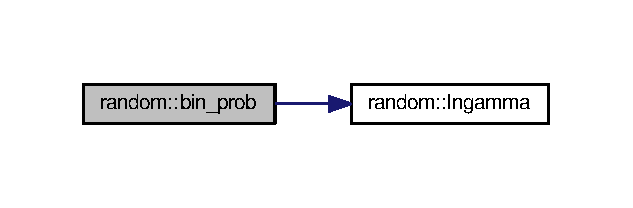
\includegraphics[width=304pt]{classrandom_a09f3df72ead2420edd0672a21a7d210e_cgraph}
\end{center}
\end{figure}




Here is the caller graph for this function\-:\nopagebreak
\begin{figure}[H]
\begin{center}
\leavevmode
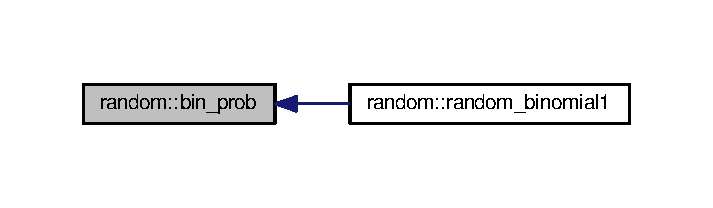
\includegraphics[width=342pt]{classrandom_a09f3df72ead2420edd0672a21a7d210e_icgraph}
\end{center}
\end{figure}


\hypertarget{classrandom_aeb29b320c803774e82f6245ad6f33aae}{\index{random@{random}!lngamma@{lngamma}}
\index{lngamma@{lngamma}!random@{random}}
\subsubsection[{lngamma}]{\setlength{\rightskip}{0pt plus 5cm}real ({\bf dp}) function random\-::lngamma (
\begin{DoxyParamCaption}
\item[{real ({\bf dp}), intent(in)}]{x}
\end{DoxyParamCaption}
)}}\label{classrandom_aeb29b320c803774e82f6245ad6f33aae}


Here is the caller graph for this function\-:\nopagebreak
\begin{figure}[H]
\begin{center}
\leavevmode
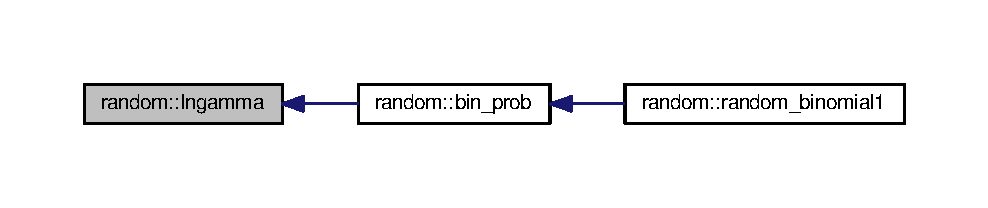
\includegraphics[width=350pt]{classrandom_aeb29b320c803774e82f6245ad6f33aae_icgraph}
\end{center}
\end{figure}


\hypertarget{classrandom_a0037b9f6838b023c794c2addf89f9ba1}{\index{random@{random}!random\-\_\-beta@{random\-\_\-beta}}
\index{random\-\_\-beta@{random\-\_\-beta}!random@{random}}
\subsubsection[{random\-\_\-beta}]{\setlength{\rightskip}{0pt plus 5cm}real(kind=kind(1.\-0d+0)) function random\-::random\-\_\-beta (
\begin{DoxyParamCaption}
\item[{real(kind=kind(1.\-0d+0)), intent(in)}]{aa, }
\item[{real(kind=kind(1.\-0d+0)), intent(in)}]{bb, }
\item[{logical, intent(in)}]{first}
\end{DoxyParamCaption}
)}}\label{classrandom_a0037b9f6838b023c794c2addf89f9ba1}
\hypertarget{classrandom_a9d4c34e7ad5aab9e084465c7842d1a8a}{\index{random@{random}!random\-\_\-binomial1@{random\-\_\-binomial1}}
\index{random\-\_\-binomial1@{random\-\_\-binomial1}!random@{random}}
\subsubsection[{random\-\_\-binomial1}]{\setlength{\rightskip}{0pt plus 5cm}integer function random\-::random\-\_\-binomial1 (
\begin{DoxyParamCaption}
\item[{integer, intent(in)}]{n, }
\item[{real(kind=kind(1.\-0d+0)), intent(in)}]{p, }
\item[{logical, intent(in)}]{first}
\end{DoxyParamCaption}
)}}\label{classrandom_a9d4c34e7ad5aab9e084465c7842d1a8a}


Here is the call graph for this function\-:\nopagebreak
\begin{figure}[H]
\begin{center}
\leavevmode
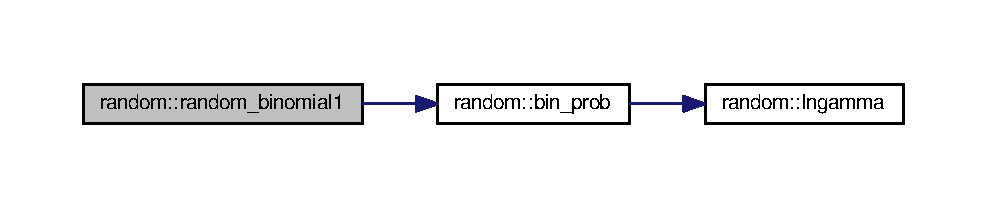
\includegraphics[width=350pt]{classrandom_a9d4c34e7ad5aab9e084465c7842d1a8a_cgraph}
\end{center}
\end{figure}


\hypertarget{classrandom_aefecf83790063d8974d72c28293f2413}{\index{random@{random}!random\-\_\-binomial2@{random\-\_\-binomial2}}
\index{random\-\_\-binomial2@{random\-\_\-binomial2}!random@{random}}
\subsubsection[{random\-\_\-binomial2}]{\setlength{\rightskip}{0pt plus 5cm}integer function random\-::random\-\_\-binomial2 (
\begin{DoxyParamCaption}
\item[{integer, intent(in)}]{n, }
\item[{real(kind=kind(1.\-0d+0)), intent(in)}]{pp, }
\item[{logical, intent(in)}]{first}
\end{DoxyParamCaption}
)}}\label{classrandom_aefecf83790063d8974d72c28293f2413}


Here is the call graph for this function\-:\nopagebreak
\begin{figure}[H]
\begin{center}
\leavevmode
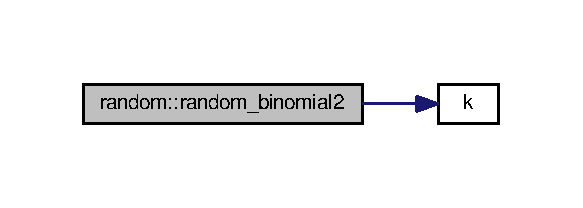
\includegraphics[width=280pt]{classrandom_aefecf83790063d8974d72c28293f2413_cgraph}
\end{center}
\end{figure}


\hypertarget{classrandom_a812d6055f4c3c34177a7681a2302b03b}{\index{random@{random}!random\-\_\-cauchy@{random\-\_\-cauchy}}
\index{random\-\_\-cauchy@{random\-\_\-cauchy}!random@{random}}
\subsubsection[{random\-\_\-cauchy}]{\setlength{\rightskip}{0pt plus 5cm}real(kind=kind(1.\-0d+0)) function random\-::random\-\_\-cauchy (
\begin{DoxyParamCaption}
{}
\end{DoxyParamCaption}
)}}\label{classrandom_a812d6055f4c3c34177a7681a2302b03b}
\hypertarget{classrandom_ac6329ddadc01dc01d991971b5d955727}{\index{random@{random}!random\-\_\-chisq@{random\-\_\-chisq}}
\index{random\-\_\-chisq@{random\-\_\-chisq}!random@{random}}
\subsubsection[{random\-\_\-chisq}]{\setlength{\rightskip}{0pt plus 5cm}real(kind=kind(1.\-0d+0)) function random\-::random\-\_\-chisq (
\begin{DoxyParamCaption}
\item[{integer, intent(in)}]{ndf, }
\item[{logical, intent(in)}]{first}
\end{DoxyParamCaption}
)}}\label{classrandom_ac6329ddadc01dc01d991971b5d955727}


Here is the call graph for this function\-:\nopagebreak
\begin{figure}[H]
\begin{center}
\leavevmode
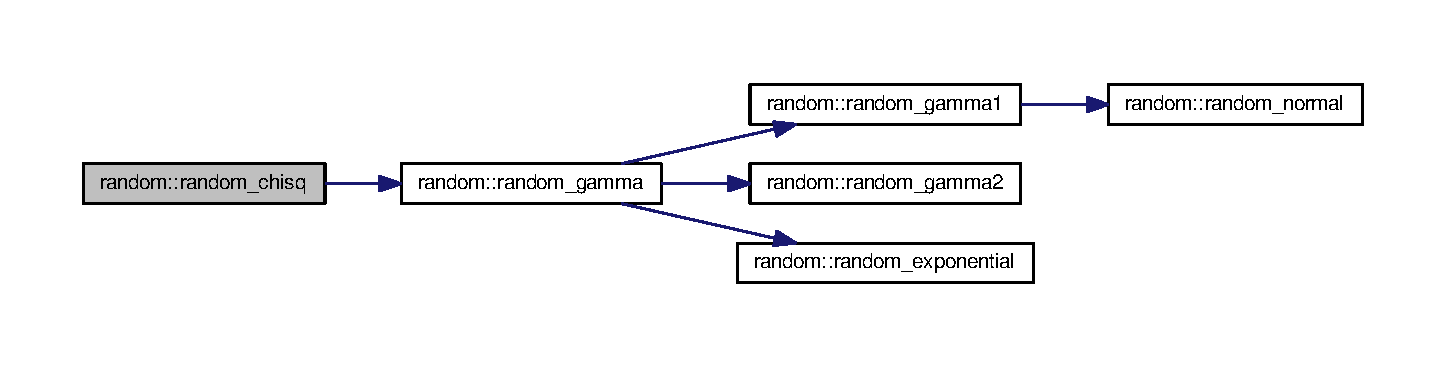
\includegraphics[width=350pt]{classrandom_ac6329ddadc01dc01d991971b5d955727_cgraph}
\end{center}
\end{figure}


\hypertarget{classrandom_a14421c1b908f2263d65da068fddfc7dd}{\index{random@{random}!random\-\_\-exponential@{random\-\_\-exponential}}
\index{random\-\_\-exponential@{random\-\_\-exponential}!random@{random}}
\subsubsection[{random\-\_\-exponential}]{\setlength{\rightskip}{0pt plus 5cm}real(kind=kind(1.\-0d+0)) function random\-::random\-\_\-exponential (
\begin{DoxyParamCaption}
{}
\end{DoxyParamCaption}
)}}\label{classrandom_a14421c1b908f2263d65da068fddfc7dd}


Here is the caller graph for this function\-:\nopagebreak
\begin{figure}[H]
\begin{center}
\leavevmode
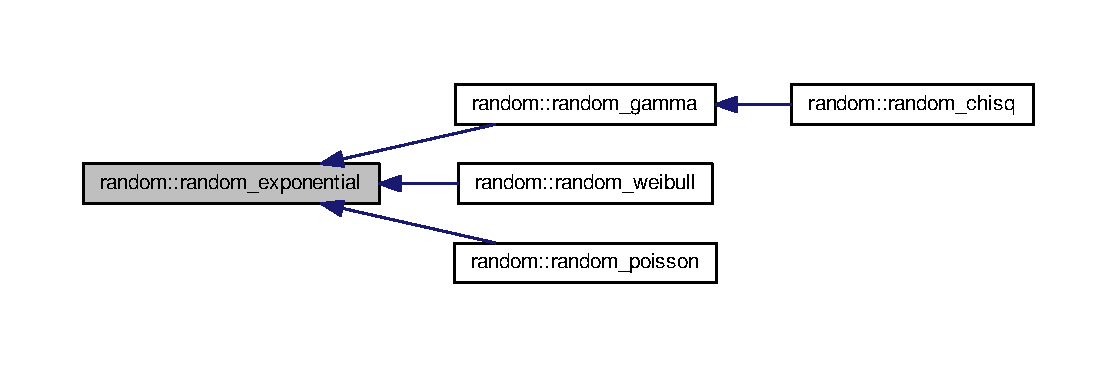
\includegraphics[width=350pt]{classrandom_a14421c1b908f2263d65da068fddfc7dd_icgraph}
\end{center}
\end{figure}


\hypertarget{classrandom_a0ffe848e8b744d46f54c64489374cadf}{\index{random@{random}!random\-\_\-gamma@{random\-\_\-gamma}}
\index{random\-\_\-gamma@{random\-\_\-gamma}!random@{random}}
\subsubsection[{random\-\_\-gamma}]{\setlength{\rightskip}{0pt plus 5cm}real(kind=kind(1.\-0d+0)) function random\-::random\-\_\-gamma (
\begin{DoxyParamCaption}
\item[{real(kind=kind(1.\-0d+0)), intent(in)}]{s, }
\item[{logical, intent(in)}]{first}
\end{DoxyParamCaption}
)}}\label{classrandom_a0ffe848e8b744d46f54c64489374cadf}


Here is the call graph for this function\-:\nopagebreak
\begin{figure}[H]
\begin{center}
\leavevmode
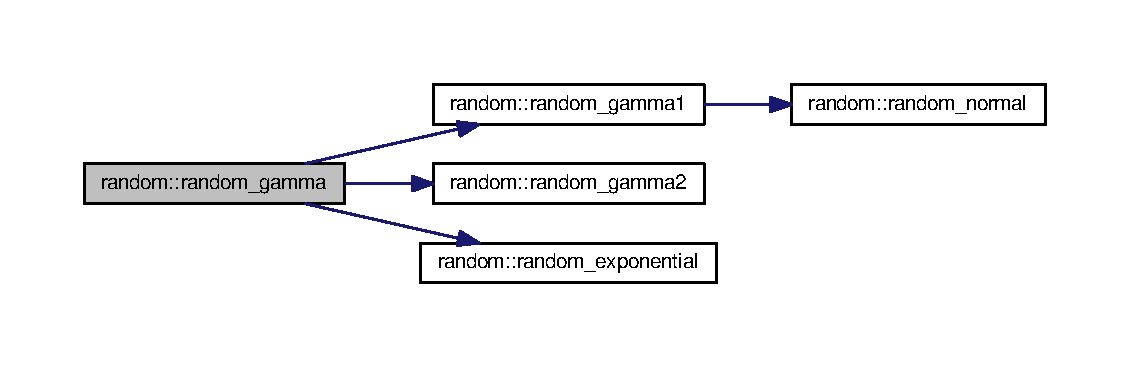
\includegraphics[width=350pt]{classrandom_a0ffe848e8b744d46f54c64489374cadf_cgraph}
\end{center}
\end{figure}




Here is the caller graph for this function\-:\nopagebreak
\begin{figure}[H]
\begin{center}
\leavevmode
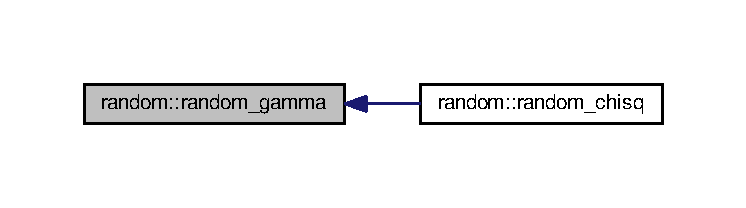
\includegraphics[width=350pt]{classrandom_a0ffe848e8b744d46f54c64489374cadf_icgraph}
\end{center}
\end{figure}


\hypertarget{classrandom_a7f62d97723dd55391a86b2875b8f67b1}{\index{random@{random}!random\-\_\-gamma1@{random\-\_\-gamma1}}
\index{random\-\_\-gamma1@{random\-\_\-gamma1}!random@{random}}
\subsubsection[{random\-\_\-gamma1}]{\setlength{\rightskip}{0pt plus 5cm}real(kind=kind(1.\-0d+0)) function random\-::random\-\_\-gamma1 (
\begin{DoxyParamCaption}
\item[{real(kind=kind(1.\-0d+0)), intent(in)}]{s, }
\item[{logical, intent(in)}]{first}
\end{DoxyParamCaption}
)}}\label{classrandom_a7f62d97723dd55391a86b2875b8f67b1}


Here is the call graph for this function\-:\nopagebreak
\begin{figure}[H]
\begin{center}
\leavevmode
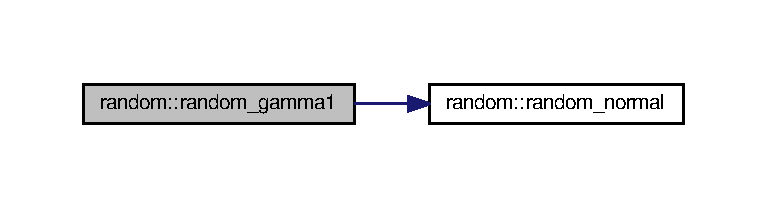
\includegraphics[width=350pt]{classrandom_a7f62d97723dd55391a86b2875b8f67b1_cgraph}
\end{center}
\end{figure}




Here is the caller graph for this function\-:\nopagebreak
\begin{figure}[H]
\begin{center}
\leavevmode
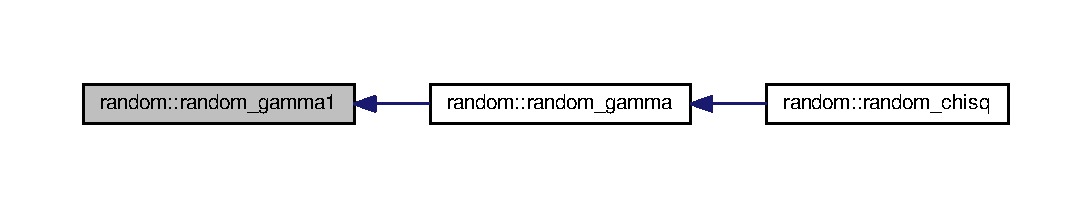
\includegraphics[width=350pt]{classrandom_a7f62d97723dd55391a86b2875b8f67b1_icgraph}
\end{center}
\end{figure}


\hypertarget{classrandom_a6c16fa1e3c755b37dc43212078c6af18}{\index{random@{random}!random\-\_\-gamma2@{random\-\_\-gamma2}}
\index{random\-\_\-gamma2@{random\-\_\-gamma2}!random@{random}}
\subsubsection[{random\-\_\-gamma2}]{\setlength{\rightskip}{0pt plus 5cm}real(kind=kind(1.\-0d+0)) function random\-::random\-\_\-gamma2 (
\begin{DoxyParamCaption}
\item[{real(kind=kind(1.\-0d+0)), intent(in)}]{s, }
\item[{logical, intent(in)}]{first}
\end{DoxyParamCaption}
)}}\label{classrandom_a6c16fa1e3c755b37dc43212078c6af18}


Here is the caller graph for this function\-:\nopagebreak
\begin{figure}[H]
\begin{center}
\leavevmode
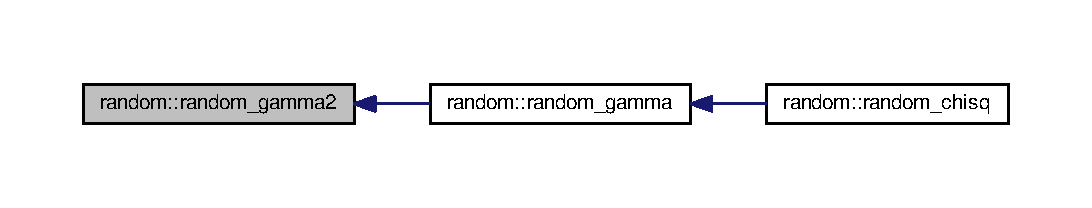
\includegraphics[width=350pt]{classrandom_a6c16fa1e3c755b37dc43212078c6af18_icgraph}
\end{center}
\end{figure}


\hypertarget{classrandom_a238863a66d36cc568a878418c31e96b4}{\index{random@{random}!random\-\_\-inv\-\_\-gauss@{random\-\_\-inv\-\_\-gauss}}
\index{random\-\_\-inv\-\_\-gauss@{random\-\_\-inv\-\_\-gauss}!random@{random}}
\subsubsection[{random\-\_\-inv\-\_\-gauss}]{\setlength{\rightskip}{0pt plus 5cm}real(kind=kind(1.\-0d+0)) function random\-::random\-\_\-inv\-\_\-gauss (
\begin{DoxyParamCaption}
\item[{real(kind=kind(1.\-0d+0)), intent(in)}]{h, }
\item[{real(kind=kind(1.\-0d+0)), intent(in)}]{b, }
\item[{logical, intent(in)}]{first}
\end{DoxyParamCaption}
)}}\label{classrandom_a238863a66d36cc568a878418c31e96b4}
\hypertarget{classrandom_a2770bb736479f52377a6f9eea473da8e}{\index{random@{random}!random\-\_\-mvnorm@{random\-\_\-mvnorm}}
\index{random\-\_\-mvnorm@{random\-\_\-mvnorm}!random@{random}}
\subsubsection[{random\-\_\-mvnorm}]{\setlength{\rightskip}{0pt plus 5cm}subroutine random\-::random\-\_\-mvnorm (
\begin{DoxyParamCaption}
\item[{integer, intent(in)}]{n, }
\item[{real(kind=kind(1.\-0d+0)), dimension(\-:), intent(in)}]{h, }
\item[{real(kind=kind(1.\-0d+0)), dimension(\-:), intent(in)}]{d, }
\item[{real(kind=kind(1.\-0d+0)), dimension(\-:), intent(inout)}]{f, }
\item[{logical, intent(in)}]{first, }
\item[{real(kind=kind(1.\-0d+0)), dimension(\-:), intent(out)}]{x, }
\item[{integer, intent(out)}]{ier}
\end{DoxyParamCaption}
)}}\label{classrandom_a2770bb736479f52377a6f9eea473da8e}


Here is the call graph for this function\-:\nopagebreak
\begin{figure}[H]
\begin{center}
\leavevmode
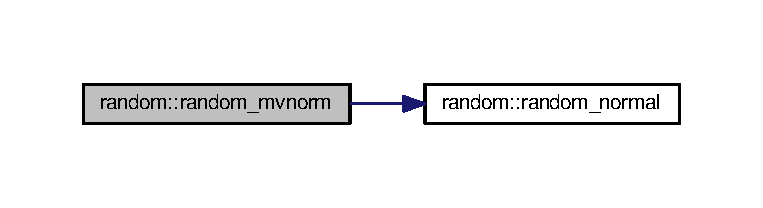
\includegraphics[width=350pt]{classrandom_a2770bb736479f52377a6f9eea473da8e_cgraph}
\end{center}
\end{figure}


\hypertarget{classrandom_a3107e0ecaf18a7095150c0f911aac145}{\index{random@{random}!random\-\_\-neg\-\_\-binomial@{random\-\_\-neg\-\_\-binomial}}
\index{random\-\_\-neg\-\_\-binomial@{random\-\_\-neg\-\_\-binomial}!random@{random}}
\subsubsection[{random\-\_\-neg\-\_\-binomial}]{\setlength{\rightskip}{0pt plus 5cm}integer function random\-::random\-\_\-neg\-\_\-binomial (
\begin{DoxyParamCaption}
\item[{real(kind=kind(1.\-0d+0)), intent(in)}]{sk, }
\item[{real(kind=kind(1.\-0d+0)), intent(in)}]{p}
\end{DoxyParamCaption}
)}}\label{classrandom_a3107e0ecaf18a7095150c0f911aac145}


Here is the call graph for this function\-:\nopagebreak
\begin{figure}[H]
\begin{center}
\leavevmode
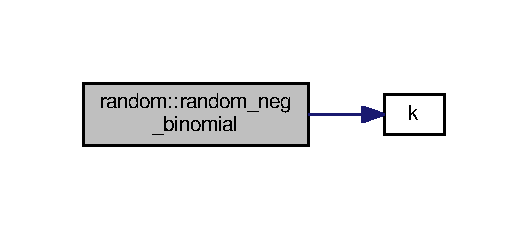
\includegraphics[width=254pt]{classrandom_a3107e0ecaf18a7095150c0f911aac145_cgraph}
\end{center}
\end{figure}


\hypertarget{classrandom_a05c493f12b4a3acad4d42bf23e3bf23a}{\index{random@{random}!random\-\_\-normal@{random\-\_\-normal}}
\index{random\-\_\-normal@{random\-\_\-normal}!random@{random}}
\subsubsection[{random\-\_\-normal}]{\setlength{\rightskip}{0pt plus 5cm}real(kind=kind(1.\-0d+0)) function random\-::random\-\_\-normal (
\begin{DoxyParamCaption}
{}
\end{DoxyParamCaption}
)}}\label{classrandom_a05c493f12b4a3acad4d42bf23e3bf23a}


function to get random normal with zero mean and stdev 1 

\begin{DoxyReturn}{Returns}
fn\-\_\-val 
\end{DoxyReturn}


Here is the caller graph for this function\-:\nopagebreak
\begin{figure}[H]
\begin{center}
\leavevmode
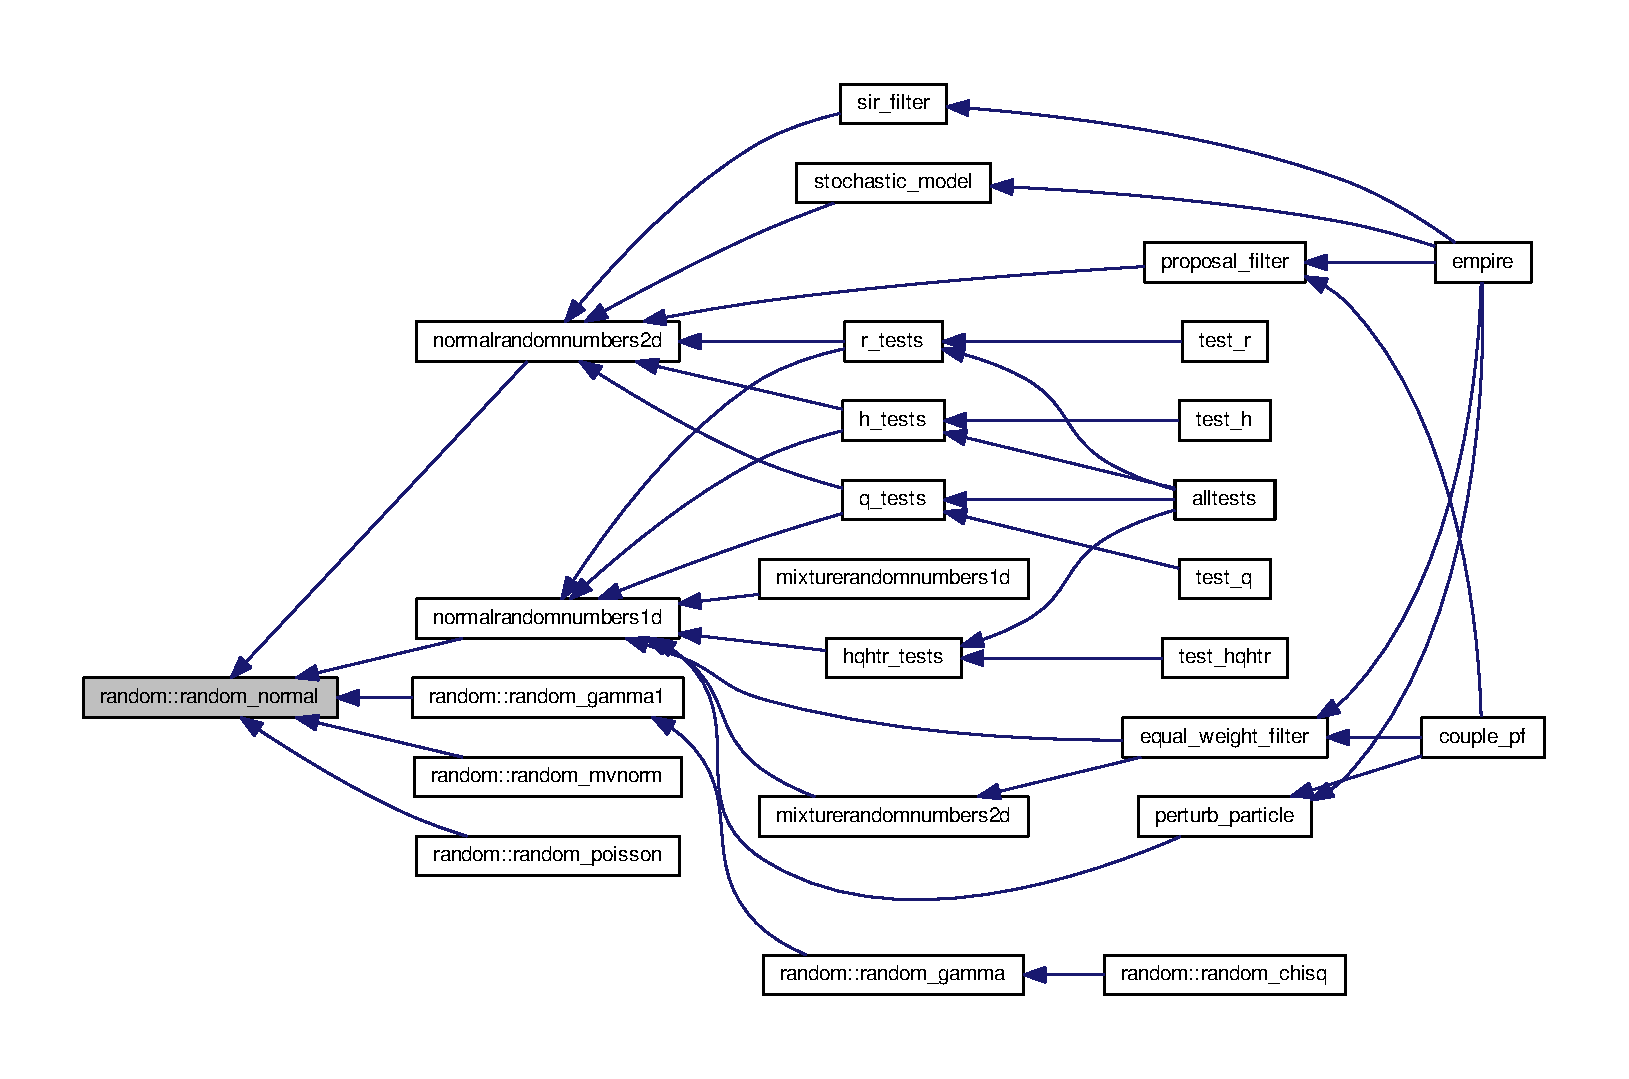
\includegraphics[width=350pt]{classrandom_a05c493f12b4a3acad4d42bf23e3bf23a_icgraph}
\end{center}
\end{figure}


\hypertarget{classrandom_a03e6b0b30475831f6d57082faed3bb34}{\index{random@{random}!random\-\_\-order@{random\-\_\-order}}
\index{random\-\_\-order@{random\-\_\-order}!random@{random}}
\subsubsection[{random\-\_\-order}]{\setlength{\rightskip}{0pt plus 5cm}subroutine random\-::random\-\_\-order (
\begin{DoxyParamCaption}
\item[{integer, dimension(n), intent(out)}]{order, }
\item[{integer, intent(in)}]{n}
\end{DoxyParamCaption}
)}}\label{classrandom_a03e6b0b30475831f6d57082faed3bb34}


Here is the call graph for this function\-:\nopagebreak
\begin{figure}[H]
\begin{center}
\leavevmode
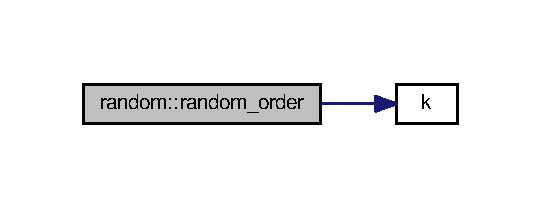
\includegraphics[width=260pt]{classrandom_a03e6b0b30475831f6d57082faed3bb34_cgraph}
\end{center}
\end{figure}


\hypertarget{classrandom_a4ec519e7171cd11a636820c235a04e97}{\index{random@{random}!random\-\_\-poisson@{random\-\_\-poisson}}
\index{random\-\_\-poisson@{random\-\_\-poisson}!random@{random}}
\subsubsection[{random\-\_\-poisson}]{\setlength{\rightskip}{0pt plus 5cm}integer function random\-::random\-\_\-poisson (
\begin{DoxyParamCaption}
\item[{real(kind=kind(1.\-0d+0)), intent(in)}]{mu, }
\item[{logical, intent(in)}]{first}
\end{DoxyParamCaption}
)}}\label{classrandom_a4ec519e7171cd11a636820c235a04e97}


Here is the call graph for this function\-:\nopagebreak
\begin{figure}[H]
\begin{center}
\leavevmode
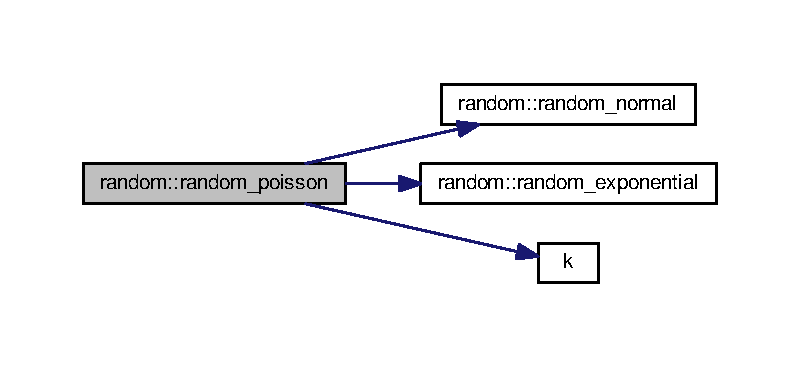
\includegraphics[width=350pt]{classrandom_a4ec519e7171cd11a636820c235a04e97_cgraph}
\end{center}
\end{figure}


\hypertarget{classrandom_a52f7096c93579e684fd894e01bedcd4d}{\index{random@{random}!random\-\_\-t@{random\-\_\-t}}
\index{random\-\_\-t@{random\-\_\-t}!random@{random}}
\subsubsection[{random\-\_\-t}]{\setlength{\rightskip}{0pt plus 5cm}real(kind=kind(1.\-0d+0)) function random\-::random\-\_\-t (
\begin{DoxyParamCaption}
\item[{integer, intent(in)}]{m}
\end{DoxyParamCaption}
)}}\label{classrandom_a52f7096c93579e684fd894e01bedcd4d}
\hypertarget{classrandom_ae89f09ae700db89c4e3593dda9e4d334}{\index{random@{random}!random\-\_\-von\-\_\-mises@{random\-\_\-von\-\_\-mises}}
\index{random\-\_\-von\-\_\-mises@{random\-\_\-von\-\_\-mises}!random@{random}}
\subsubsection[{random\-\_\-von\-\_\-mises}]{\setlength{\rightskip}{0pt plus 5cm}real(kind=kind(1.\-0d+0)) function random\-::random\-\_\-von\-\_\-mises (
\begin{DoxyParamCaption}
\item[{real(kind=kind(1.\-0d+0)), intent(in)}]{k, }
\item[{logical, intent(in)}]{first}
\end{DoxyParamCaption}
)}}\label{classrandom_ae89f09ae700db89c4e3593dda9e4d334}


Here is the call graph for this function\-:\nopagebreak
\begin{figure}[H]
\begin{center}
\leavevmode
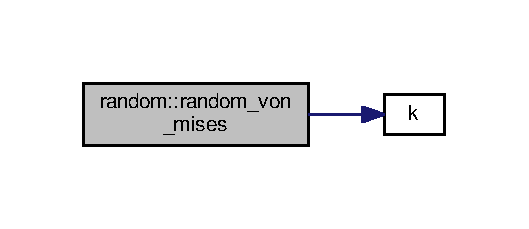
\includegraphics[width=254pt]{classrandom_ae89f09ae700db89c4e3593dda9e4d334_cgraph}
\end{center}
\end{figure}


\hypertarget{classrandom_ab847036d4dbe5c63613425d28a395275}{\index{random@{random}!random\-\_\-weibull@{random\-\_\-weibull}}
\index{random\-\_\-weibull@{random\-\_\-weibull}!random@{random}}
\subsubsection[{random\-\_\-weibull}]{\setlength{\rightskip}{0pt plus 5cm}real(kind=kind(1.\-0d+0)) function random\-::random\-\_\-weibull (
\begin{DoxyParamCaption}
\item[{real(kind=kind(1.\-0d+0)), intent(in)}]{a}
\end{DoxyParamCaption}
)}}\label{classrandom_ab847036d4dbe5c63613425d28a395275}


Here is the call graph for this function\-:\nopagebreak
\begin{figure}[H]
\begin{center}
\leavevmode
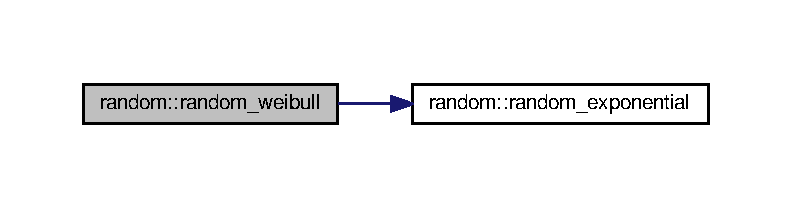
\includegraphics[width=350pt]{classrandom_ab847036d4dbe5c63613425d28a395275_cgraph}
\end{center}
\end{figure}


\hypertarget{classrandom_a82f08f6c9b3c4740501abb1970397f8d}{\index{random@{random}!seed\-\_\-random\-\_\-number@{seed\-\_\-random\-\_\-number}}
\index{seed\-\_\-random\-\_\-number@{seed\-\_\-random\-\_\-number}!random@{random}}
\subsubsection[{seed\-\_\-random\-\_\-number}]{\setlength{\rightskip}{0pt plus 5cm}subroutine random\-::seed\-\_\-random\-\_\-number (
\begin{DoxyParamCaption}
\item[{integer, intent(in)}]{iounit}
\end{DoxyParamCaption}
)}}\label{classrandom_a82f08f6c9b3c4740501abb1970397f8d}


Here is the call graph for this function\-:\nopagebreak
\begin{figure}[H]
\begin{center}
\leavevmode
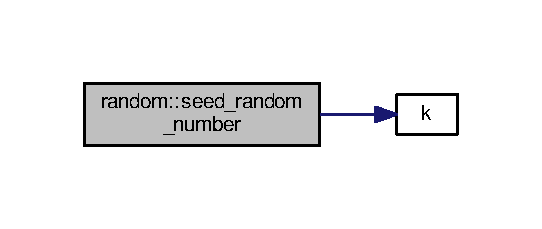
\includegraphics[width=260pt]{classrandom_a82f08f6c9b3c4740501abb1970397f8d_cgraph}
\end{center}
\end{figure}




\subsection{Member Data Documentation}
\hypertarget{classrandom_a0026984dfe1c95755ce81e2372a06f22}{\index{random@{random}!dp@{dp}}
\index{dp@{dp}!random@{random}}
\subsubsection[{dp}]{\setlength{\rightskip}{0pt plus 5cm}integer, parameter random\-::dp = S\-E\-L\-E\-C\-T\-E\-D\-\_\-\-R\-E\-A\-L\-\_\-\-K\-I\-N\-D(12, 60)}}\label{classrandom_a0026984dfe1c95755ce81e2372a06f22}


The documentation for this module was generated from the following file\-:\begin{DoxyCompactItemize}
\item 
src/utils/\hyperlink{random__d_8f90}{random\-\_\-d.\-f90}\end{DoxyCompactItemize}

\hypertarget{classrdata}{\section{rdata Module Reference}
\label{classrdata}\index{rdata@{rdata}}
}


Module to hold user supplied data for $R$ observation error covariance matrix.  


\subsection*{Public Member Functions}
\begin{DoxyCompactItemize}
\item 
subroutine \hyperlink{classrdata_a10ee06d3ab047a5b82de8d8ee1f6b76e}{loadr}
\begin{DoxyCompactList}\small\item\em Subroutine to load data for R. \end{DoxyCompactList}\item 
subroutine \hyperlink{classrdata_a9236685f842c013fb282e4eb3f5430aa}{killr}
\end{DoxyCompactItemize}
\subsection*{Public Attributes}
\begin{DoxyCompactItemize}
\item 
integer \hyperlink{classrdata_a9a5360e6be18637e65fcae5c55d8db98}{rn}
\item 
integer \hyperlink{classrdata_ae2a9f3970d94f6130c3dfd4f3f955768}{rne}
\item 
integer, dimension(\-:), allocatable \hyperlink{classrdata_aa0e9818ee0a39f028d35cd48a32e5cba}{rrow}
\item 
integer, dimension(\-:), allocatable \hyperlink{classrdata_a293ef50d8603271fa571f705f4d774d4}{rcol}
\item 
real(kind=kind(1.\-0d0)), dimension(\-:), allocatable \hyperlink{classrdata_ae49a7ea0826ee25bffa2ed191b07cbb3}{rval}
\item 
real(kind=kind(1.\-0d0)), dimension(\-:), allocatable \hyperlink{classrdata_a89b639fead94b96b7f5d6aef6a7a449a}{rdiag}
\end{DoxyCompactItemize}


\subsection{Detailed Description}
Module to hold user supplied data for $R$ observation error covariance matrix. 

\subsection{Member Function/\-Subroutine Documentation}
\hypertarget{classrdata_a9236685f842c013fb282e4eb3f5430aa}{\index{rdata@{rdata}!killr@{killr}}
\index{killr@{killr}!rdata@{rdata}}
\subsubsection[{killr}]{\setlength{\rightskip}{0pt plus 5cm}subroutine rdata\-::killr (
\begin{DoxyParamCaption}
{}
\end{DoxyParamCaption}
)}}\label{classrdata_a9236685f842c013fb282e4eb3f5430aa}
S\-Ubroutine to deallocate R data \hypertarget{classrdata_a10ee06d3ab047a5b82de8d8ee1f6b76e}{\index{rdata@{rdata}!loadr@{loadr}}
\index{loadr@{loadr}!rdata@{rdata}}
\subsubsection[{loadr}]{\setlength{\rightskip}{0pt plus 5cm}subroutine rdata\-::loadr (
\begin{DoxyParamCaption}
{}
\end{DoxyParamCaption}
)}}\label{classrdata_a10ee06d3ab047a5b82de8d8ee1f6b76e}


Subroutine to load data for R. 



\subsection{Member Data Documentation}
\hypertarget{classrdata_a293ef50d8603271fa571f705f4d774d4}{\index{rdata@{rdata}!rcol@{rcol}}
\index{rcol@{rcol}!rdata@{rdata}}
\subsubsection[{rcol}]{\setlength{\rightskip}{0pt plus 5cm}integer, dimension(\-:), allocatable rdata\-::rcol}}\label{classrdata_a293ef50d8603271fa571f705f4d774d4}
\hypertarget{classrdata_a89b639fead94b96b7f5d6aef6a7a449a}{\index{rdata@{rdata}!rdiag@{rdiag}}
\index{rdiag@{rdiag}!rdata@{rdata}}
\subsubsection[{rdiag}]{\setlength{\rightskip}{0pt plus 5cm}real(kind=kind(1.\-0d0)), dimension(\-:), allocatable rdata\-::rdiag}}\label{classrdata_a89b639fead94b96b7f5d6aef6a7a449a}
\hypertarget{classrdata_a9a5360e6be18637e65fcae5c55d8db98}{\index{rdata@{rdata}!rn@{rn}}
\index{rn@{rn}!rdata@{rdata}}
\subsubsection[{rn}]{\setlength{\rightskip}{0pt plus 5cm}integer rdata\-::rn}}\label{classrdata_a9a5360e6be18637e65fcae5c55d8db98}
\hypertarget{classrdata_ae2a9f3970d94f6130c3dfd4f3f955768}{\index{rdata@{rdata}!rne@{rne}}
\index{rne@{rne}!rdata@{rdata}}
\subsubsection[{rne}]{\setlength{\rightskip}{0pt plus 5cm}integer rdata\-::rne}}\label{classrdata_ae2a9f3970d94f6130c3dfd4f3f955768}
\hypertarget{classrdata_aa0e9818ee0a39f028d35cd48a32e5cba}{\index{rdata@{rdata}!rrow@{rrow}}
\index{rrow@{rrow}!rdata@{rdata}}
\subsubsection[{rrow}]{\setlength{\rightskip}{0pt plus 5cm}integer, dimension(\-:), allocatable rdata\-::rrow}}\label{classrdata_aa0e9818ee0a39f028d35cd48a32e5cba}
\hypertarget{classrdata_ae49a7ea0826ee25bffa2ed191b07cbb3}{\index{rdata@{rdata}!rval@{rval}}
\index{rval@{rval}!rdata@{rdata}}
\subsubsection[{rval}]{\setlength{\rightskip}{0pt plus 5cm}real(kind=kind(1.\-0d0)), dimension(\-:), allocatable rdata\-::rval}}\label{classrdata_ae49a7ea0826ee25bffa2ed191b07cbb3}


The documentation for this module was generated from the following file\-:\begin{DoxyCompactItemize}
\item 
src/data/\hyperlink{_rdata_8f90}{Rdata.\-f90}\end{DoxyCompactItemize}

\hypertarget{classsizes}{\section{sizes Module Reference}
\label{classsizes}\index{sizes@{sizes}}
}


Module that stores the dimension of observation and state spaces.  


\subsection*{Public Attributes}
\begin{DoxyCompactItemize}
\item 
integer \hyperlink{classsizes_a5f5dd89a39d1254b4ac7f7daf2280518}{obs\-\_\-dim}
\begin{DoxyCompactList}\small\item\em size of the observation space \end{DoxyCompactList}\item 
integer \hyperlink{classsizes_a53ccc50a0ecaf0a8601298c8c5d7ad63}{state\-\_\-dim}
\begin{DoxyCompactList}\small\item\em dimension of the model \end{DoxyCompactList}\end{DoxyCompactItemize}


\subsection{Detailed Description}
Module that stores the dimension of observation and state spaces. 

\subsection{Member Data Documentation}
\hypertarget{classsizes_a5f5dd89a39d1254b4ac7f7daf2280518}{\index{sizes@{sizes}!obs\-\_\-dim@{obs\-\_\-dim}}
\index{obs\-\_\-dim@{obs\-\_\-dim}!sizes@{sizes}}
\subsubsection[{obs\-\_\-dim}]{\setlength{\rightskip}{0pt plus 5cm}integer sizes\-::obs\-\_\-dim}}\label{classsizes_a5f5dd89a39d1254b4ac7f7daf2280518}


size of the observation space 

\hypertarget{classsizes_a53ccc50a0ecaf0a8601298c8c5d7ad63}{\index{sizes@{sizes}!state\-\_\-dim@{state\-\_\-dim}}
\index{state\-\_\-dim@{state\-\_\-dim}!sizes@{sizes}}
\subsubsection[{state\-\_\-dim}]{\setlength{\rightskip}{0pt plus 5cm}integer sizes\-::state\-\_\-dim}}\label{classsizes_a53ccc50a0ecaf0a8601298c8c5d7ad63}


dimension of the model 



The documentation for this module was generated from the following file\-:\begin{DoxyCompactItemize}
\item 
src/controlers/\hyperlink{sizes_8f90}{sizes.\-f90}\end{DoxyCompactItemize}

\chapter{File Documentation}
\hypertarget{old__pf__couple_8f90}{\section{src/controlers/old\-\_\-pf\-\_\-couple.f90 File Reference}
\label{old__pf__couple_8f90}\index{src/controlers/old\-\_\-pf\-\_\-couple.\-f90@{src/controlers/old\-\_\-pf\-\_\-couple.\-f90}}
}
\subsection*{Functions/\-Subroutines}
\begin{DoxyCompactItemize}
\item 
program \hyperlink{old__pf__couple_8f90_a1216ad66e8485a0af45ed20218ee2272}{couple\-\_\-pf}
\end{DoxyCompactItemize}


\subsection{Function/\-Subroutine Documentation}
\hypertarget{old__pf__couple_8f90_a1216ad66e8485a0af45ed20218ee2272}{\index{old\-\_\-pf\-\_\-couple.\-f90@{old\-\_\-pf\-\_\-couple.\-f90}!couple\-\_\-pf@{couple\-\_\-pf}}
\index{couple\-\_\-pf@{couple\-\_\-pf}!old_pf_couple.f90@{old\-\_\-pf\-\_\-couple.\-f90}}
\subsubsection[{couple\-\_\-pf}]{\setlength{\rightskip}{0pt plus 5cm}program couple\-\_\-pf (
\begin{DoxyParamCaption}
{}
\end{DoxyParamCaption}
)}}\label{old__pf__couple_8f90_a1216ad66e8485a0af45ed20218ee2272}


Here is the call graph for this function\-:\nopagebreak
\begin{figure}[H]
\begin{center}
\leavevmode
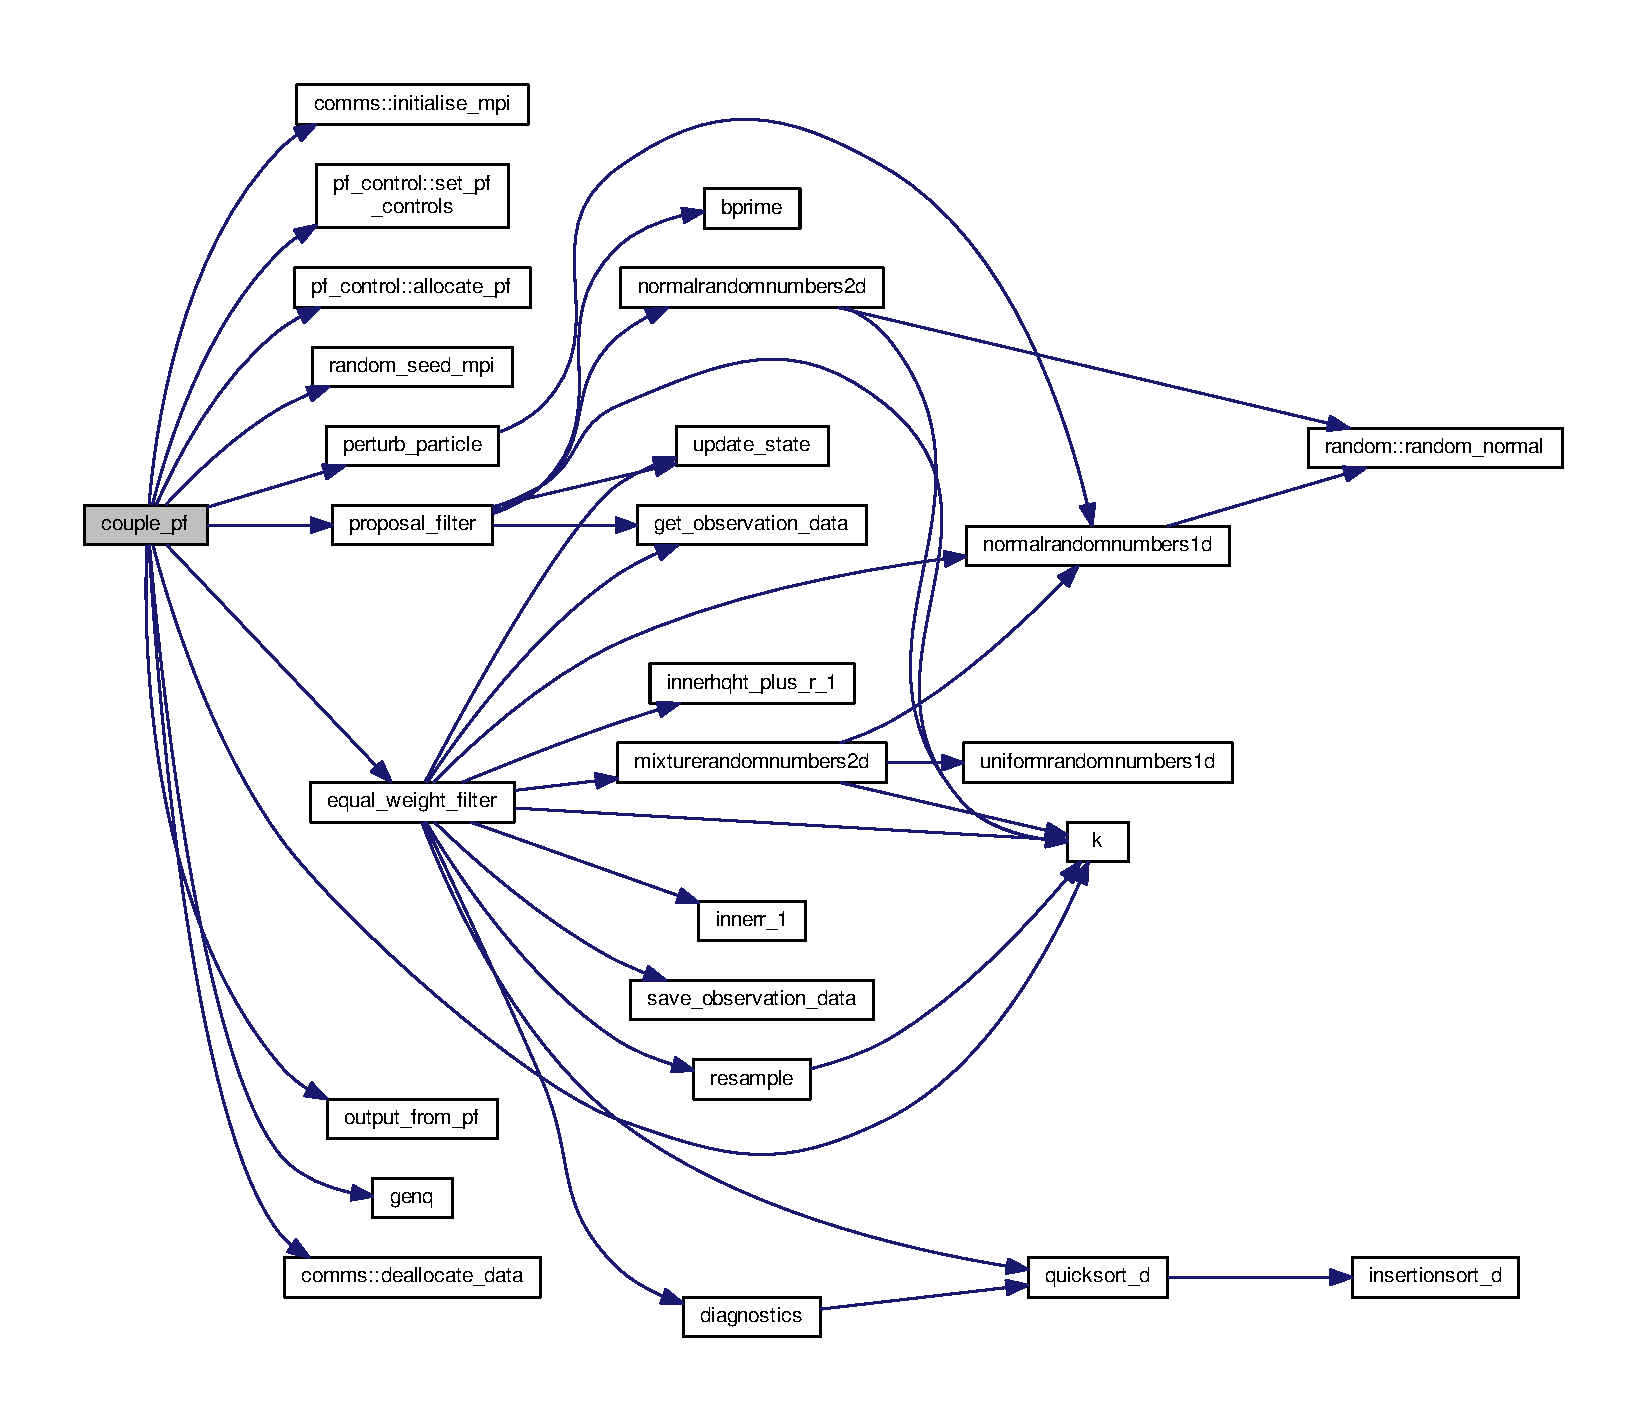
\includegraphics[width=350pt]{old__pf__couple_8f90_a1216ad66e8485a0af45ed20218ee2272_cgraph}
\end{center}
\end{figure}



\hypertarget{pf__control_8f90}{\section{src/controlers/pf\-\_\-control.f90 File Reference}
\label{pf__control_8f90}\index{src/controlers/pf\-\_\-control.\-f90@{src/controlers/pf\-\_\-control.\-f90}}
}
\subsection*{Data Types}
\begin{DoxyCompactItemize}
\item 
module \hyperlink{classpf__control}{pf\-\_\-control}
\begin{DoxyCompactList}\small\item\em module to hold all the information to control the the main program \end{DoxyCompactList}\item 
type \hyperlink{structpf__control_1_1pf__control__type}{pf\-\_\-control\-::pf\-\_\-control\-\_\-type}
\end{DoxyCompactItemize}

\hypertarget{pf__couple_8f90}{\section{src/controlers/pf\-\_\-couple.f90 File Reference}
\label{pf__couple_8f90}\index{src/controlers/pf\-\_\-couple.\-f90@{src/controlers/pf\-\_\-couple.\-f90}}
}
\subsection*{Functions/\-Subroutines}
\begin{DoxyCompactItemize}
\item 
program \hyperlink{pf__couple_8f90_a0142283b3d363fac9899bfaaf2621eae}{empire}
\begin{DoxyCompactList}\small\item\em the main program \end{DoxyCompactList}\end{DoxyCompactItemize}


\subsection{Function/\-Subroutine Documentation}
\hypertarget{pf__couple_8f90_a0142283b3d363fac9899bfaaf2621eae}{\index{pf\-\_\-couple.\-f90@{pf\-\_\-couple.\-f90}!empire@{empire}}
\index{empire@{empire}!pf_couple.f90@{pf\-\_\-couple.\-f90}}
\subsubsection[{empire}]{\setlength{\rightskip}{0pt plus 5cm}program empire (
\begin{DoxyParamCaption}
{}
\end{DoxyParamCaption}
)}}\label{pf__couple_8f90_a0142283b3d363fac9899bfaaf2621eae}


the main program 



Here is the call graph for this function\-:\nopagebreak
\begin{figure}[H]
\begin{center}
\leavevmode
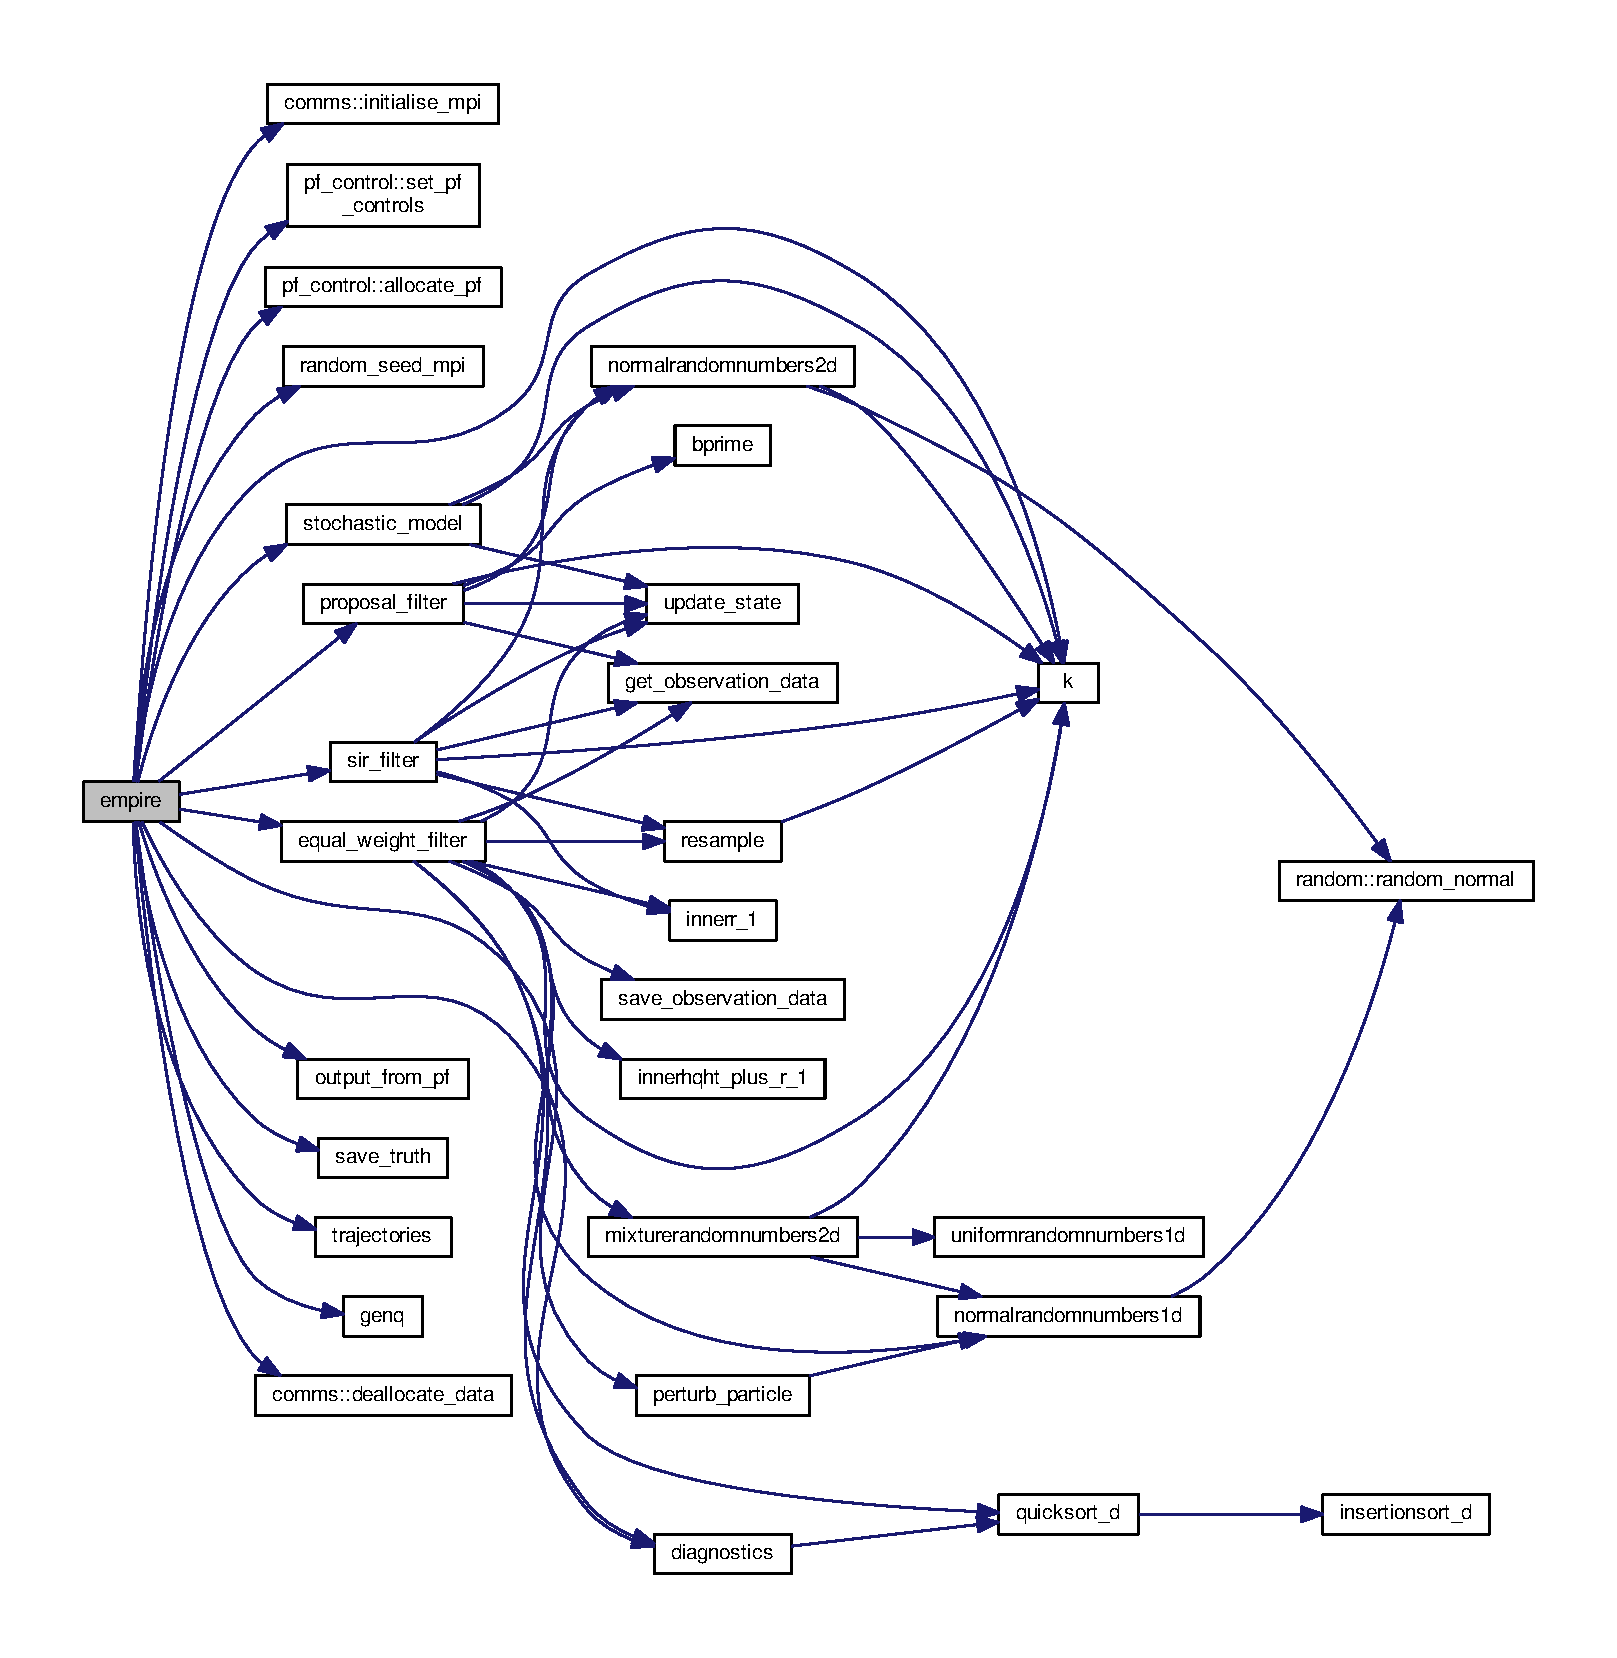
\includegraphics[width=350pt]{pf__couple_8f90_a0142283b3d363fac9899bfaaf2621eae_cgraph}
\end{center}
\end{figure}



\hypertarget{sizes_8f90}{\section{src/controlers/sizes.f90 File Reference}
\label{sizes_8f90}\index{src/controlers/sizes.\-f90@{src/controlers/sizes.\-f90}}
}
\subsection*{Data Types}
\begin{DoxyCompactItemize}
\item 
module \hyperlink{classsizes}{sizes}
\begin{DoxyCompactList}\small\item\em Module that stores the dimension of observation and state spaces. \end{DoxyCompactList}\end{DoxyCompactItemize}

\hypertarget{_qdata_8f90}{\section{src/data/\-Qdata.f90 File Reference}
\label{_qdata_8f90}\index{src/data/\-Qdata.\-f90@{src/data/\-Qdata.\-f90}}
}
\subsection*{Data Types}
\begin{DoxyCompactItemize}
\item 
module \hyperlink{classqdata}{qdata}
\begin{DoxyCompactList}\small\item\em Module as a place to store user specified data for $Q$. \end{DoxyCompactList}\end{DoxyCompactItemize}

\hypertarget{_rdata_8f90}{\section{src/data/\-Rdata.f90 File Reference}
\label{_rdata_8f90}\index{src/data/\-Rdata.\-f90@{src/data/\-Rdata.\-f90}}
}
\subsection*{Data Types}
\begin{DoxyCompactItemize}
\item 
module \hyperlink{classrdata}{rdata}
\begin{DoxyCompactList}\small\item\em Module to hold user supplied data for $R$ observation error covariance matrix. \end{DoxyCompactList}\item 
module \hyperlink{classhqht__plus__r}{hqht\-\_\-plus\-\_\-r}
\end{DoxyCompactItemize}

\hypertarget{eakf__analysis_8f90}{\section{src/filters/eakf\-\_\-analysis.f90 File Reference}
\label{eakf__analysis_8f90}\index{src/filters/eakf\-\_\-analysis.\-f90@{src/filters/eakf\-\_\-analysis.\-f90}}
}
\subsection*{Functions/\-Subroutines}
\begin{DoxyCompactItemize}
\item 
subroutine \hyperlink{eakf__analysis_8f90_a7f7aa81cc5a7a2da8f159f216e2bb156}{eakf\-\_\-analysis} (num\-\_\-hor, num\-\_\-ver, this\-\_\-hor, this\-\_\-ver, boundary, x, N, state\-Dim, obs\-Dim, rho)
\end{DoxyCompactItemize}


\subsection{Function/\-Subroutine Documentation}
\hypertarget{eakf__analysis_8f90_a7f7aa81cc5a7a2da8f159f216e2bb156}{\index{eakf\-\_\-analysis.\-f90@{eakf\-\_\-analysis.\-f90}!eakf\-\_\-analysis@{eakf\-\_\-analysis}}
\index{eakf\-\_\-analysis@{eakf\-\_\-analysis}!eakf_analysis.f90@{eakf\-\_\-analysis.\-f90}}
\subsubsection[{eakf\-\_\-analysis}]{\setlength{\rightskip}{0pt plus 5cm}subroutine eakf\-\_\-analysis (
\begin{DoxyParamCaption}
\item[{integer, intent(in)}]{num\-\_\-hor, }
\item[{integer, intent(in)}]{num\-\_\-ver, }
\item[{integer, intent(in)}]{this\-\_\-hor, }
\item[{integer, intent(in)}]{this\-\_\-ver, }
\item[{integer, intent(in)}]{boundary, }
\item[{real(kind=rk), dimension(statedim,n), intent(inout)}]{x, }
\item[{integer, intent(in)}]{N, }
\item[{integer, intent(in)}]{state\-Dim, }
\item[{integer, intent(in)}]{obs\-Dim, }
\item[{real(kind=rk), intent(in)}]{rho}
\end{DoxyParamCaption}
)}}\label{eakf__analysis_8f90_a7f7aa81cc5a7a2da8f159f216e2bb156}


Here is the call graph for this function\-:\nopagebreak
\begin{figure}[H]
\begin{center}
\leavevmode
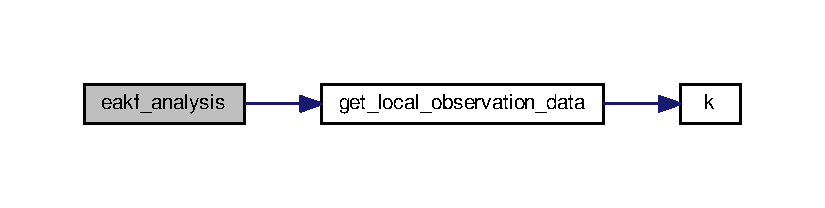
\includegraphics[width=350pt]{eakf__analysis_8f90_a7f7aa81cc5a7a2da8f159f216e2bb156_cgraph}
\end{center}
\end{figure}




Here is the caller graph for this function\-:\nopagebreak
\begin{figure}[H]
\begin{center}
\leavevmode
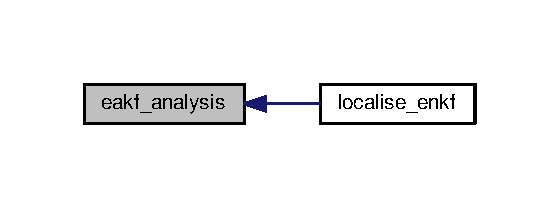
\includegraphics[width=268pt]{eakf__analysis_8f90_a7f7aa81cc5a7a2da8f159f216e2bb156_icgraph}
\end{center}
\end{figure}



\hypertarget{enkf__specific_8f90}{\section{src/filters/enkf\-\_\-specific.f90 File Reference}
\label{enkf__specific_8f90}\index{src/filters/enkf\-\_\-specific.\-f90@{src/filters/enkf\-\_\-specific.\-f90}}
}
\subsection*{Functions/\-Subroutines}
\begin{DoxyCompactItemize}
\item 
subroutine \hyperlink{enkf__specific_8f90_a135aa462c96aed62a9844af59f0eaec0}{h\-\_\-local} (num\-\_\-hor, num\-\_\-ver, this\-\_\-hor, this\-\_\-ver, boundary, nrhs, state\-Dim, x, obs\-Dim, y)
\item 
subroutine \hyperlink{enkf__specific_8f90_a391c05218787eeebf53b181156e4fcde}{solve\-\_\-rhalf\-\_\-local} (num\-\_\-hor, num\-\_\-ver, this\-\_\-hor, this\-\_\-ver, boundary, nrhs, obs\-Dim, y, v)
\item 
subroutine \hyperlink{enkf__specific_8f90_a282ddf2dfaee5bbf9982a216d58c66d4}{get\-\_\-local\-\_\-observation\-\_\-data} (num\-\_\-hor, num\-\_\-ver, this\-\_\-hor, this\-\_\-ver, boundary, obs\-Dim, y)
\item 
subroutine \hyperlink{enkf__specific_8f90_a0d5ea104a1d5bd22f8efb1c24ff2426d}{localise\-\_\-enkf} (enkf\-\_\-analysis)
\end{DoxyCompactItemize}


\subsection{Function/\-Subroutine Documentation}
\hypertarget{enkf__specific_8f90_a282ddf2dfaee5bbf9982a216d58c66d4}{\index{enkf\-\_\-specific.\-f90@{enkf\-\_\-specific.\-f90}!get\-\_\-local\-\_\-observation\-\_\-data@{get\-\_\-local\-\_\-observation\-\_\-data}}
\index{get\-\_\-local\-\_\-observation\-\_\-data@{get\-\_\-local\-\_\-observation\-\_\-data}!enkf_specific.f90@{enkf\-\_\-specific.\-f90}}
\subsubsection[{get\-\_\-local\-\_\-observation\-\_\-data}]{\setlength{\rightskip}{0pt plus 5cm}subroutine get\-\_\-local\-\_\-observation\-\_\-data (
\begin{DoxyParamCaption}
\item[{integer, intent(in)}]{num\-\_\-hor, }
\item[{integer, intent(in)}]{num\-\_\-ver, }
\item[{integer, intent(in)}]{this\-\_\-hor, }
\item[{integer, intent(in)}]{this\-\_\-ver, }
\item[{integer, intent(in)}]{boundary, }
\item[{integer, intent(in)}]{obs\-Dim, }
\item[{real(kind=rk), dimension(obsdim), intent(out)}]{y}
\end{DoxyParamCaption}
)}}\label{enkf__specific_8f90_a282ddf2dfaee5bbf9982a216d58c66d4}


Here is the call graph for this function\-:\nopagebreak
\begin{figure}[H]
\begin{center}
\leavevmode
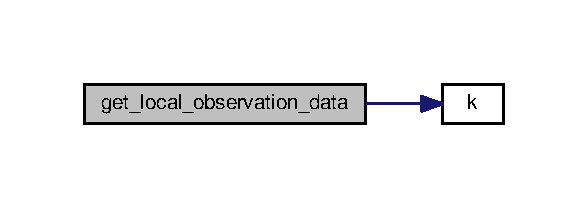
\includegraphics[width=282pt]{enkf__specific_8f90_a282ddf2dfaee5bbf9982a216d58c66d4_cgraph}
\end{center}
\end{figure}




Here is the caller graph for this function\-:\nopagebreak
\begin{figure}[H]
\begin{center}
\leavevmode
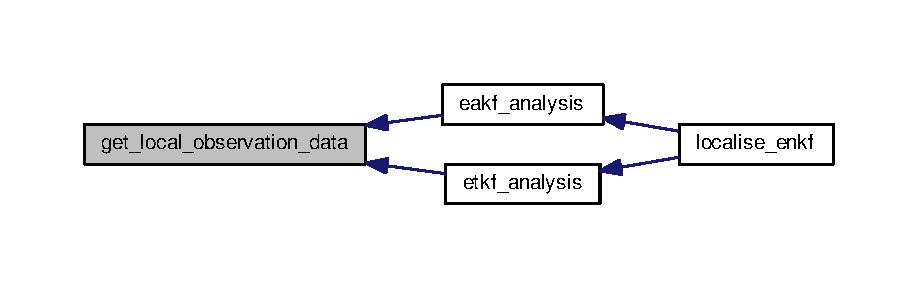
\includegraphics[width=350pt]{enkf__specific_8f90_a282ddf2dfaee5bbf9982a216d58c66d4_icgraph}
\end{center}
\end{figure}


\hypertarget{enkf__specific_8f90_a135aa462c96aed62a9844af59f0eaec0}{\index{enkf\-\_\-specific.\-f90@{enkf\-\_\-specific.\-f90}!h\-\_\-local@{h\-\_\-local}}
\index{h\-\_\-local@{h\-\_\-local}!enkf_specific.f90@{enkf\-\_\-specific.\-f90}}
\subsubsection[{h\-\_\-local}]{\setlength{\rightskip}{0pt plus 5cm}subroutine h\-\_\-local (
\begin{DoxyParamCaption}
\item[{integer, intent(in)}]{num\-\_\-hor, }
\item[{integer, intent(in)}]{num\-\_\-ver, }
\item[{integer, intent(in)}]{this\-\_\-hor, }
\item[{integer, intent(in)}]{this\-\_\-ver, }
\item[{integer, intent(in)}]{boundary, }
\item[{integer, intent(in)}]{nrhs, }
\item[{integer, intent(in)}]{state\-Dim, }
\item[{real(kind=rk), dimension(statedim,nrhs), intent(in)}]{x, }
\item[{integer, intent(in)}]{obs\-Dim, }
\item[{real(kind=rk), dimension(obsdim,nrhs), intent(out)}]{y}
\end{DoxyParamCaption}
)}}\label{enkf__specific_8f90_a135aa462c96aed62a9844af59f0eaec0}


Here is the call graph for this function\-:\nopagebreak
\begin{figure}[H]
\begin{center}
\leavevmode
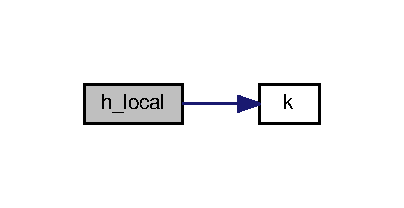
\includegraphics[width=194pt]{enkf__specific_8f90_a135aa462c96aed62a9844af59f0eaec0_cgraph}
\end{center}
\end{figure}




Here is the caller graph for this function\-:\nopagebreak
\begin{figure}[H]
\begin{center}
\leavevmode
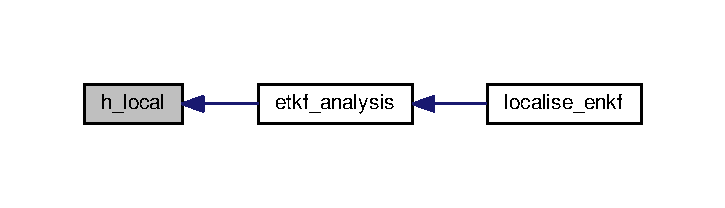
\includegraphics[width=348pt]{enkf__specific_8f90_a135aa462c96aed62a9844af59f0eaec0_icgraph}
\end{center}
\end{figure}


\hypertarget{enkf__specific_8f90_a0d5ea104a1d5bd22f8efb1c24ff2426d}{\index{enkf\-\_\-specific.\-f90@{enkf\-\_\-specific.\-f90}!localise\-\_\-enkf@{localise\-\_\-enkf}}
\index{localise\-\_\-enkf@{localise\-\_\-enkf}!enkf_specific.f90@{enkf\-\_\-specific.\-f90}}
\subsubsection[{localise\-\_\-enkf}]{\setlength{\rightskip}{0pt plus 5cm}subroutine localise\-\_\-enkf (
\begin{DoxyParamCaption}
\item[{integer, intent(in)}]{enkf\-\_\-analysis}
\end{DoxyParamCaption}
)}}\label{enkf__specific_8f90_a0d5ea104a1d5bd22f8efb1c24ff2426d}


Here is the call graph for this function\-:\nopagebreak
\begin{figure}[H]
\begin{center}
\leavevmode
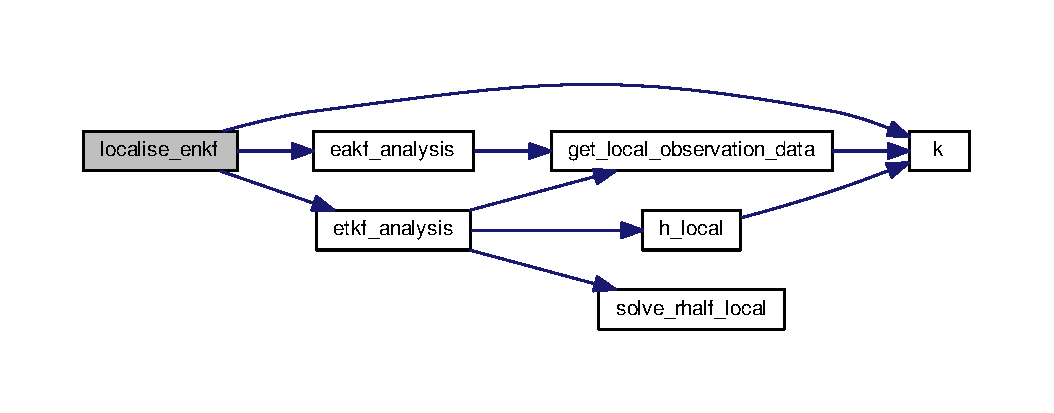
\includegraphics[width=350pt]{enkf__specific_8f90_a0d5ea104a1d5bd22f8efb1c24ff2426d_cgraph}
\end{center}
\end{figure}


\hypertarget{enkf__specific_8f90_a391c05218787eeebf53b181156e4fcde}{\index{enkf\-\_\-specific.\-f90@{enkf\-\_\-specific.\-f90}!solve\-\_\-rhalf\-\_\-local@{solve\-\_\-rhalf\-\_\-local}}
\index{solve\-\_\-rhalf\-\_\-local@{solve\-\_\-rhalf\-\_\-local}!enkf_specific.f90@{enkf\-\_\-specific.\-f90}}
\subsubsection[{solve\-\_\-rhalf\-\_\-local}]{\setlength{\rightskip}{0pt plus 5cm}subroutine solve\-\_\-rhalf\-\_\-local (
\begin{DoxyParamCaption}
\item[{integer, intent(in)}]{num\-\_\-hor, }
\item[{integer, intent(in)}]{num\-\_\-ver, }
\item[{integer, intent(in)}]{this\-\_\-hor, }
\item[{integer, intent(in)}]{this\-\_\-ver, }
\item[{integer, intent(in)}]{boundary, }
\item[{integer, intent(in)}]{nrhs, }
\item[{integer, intent(in)}]{obs\-Dim, }
\item[{real(kind=rk), dimension(obsdim,nrhs), intent(in)}]{y, }
\item[{real(kind=rk), dimension(obsdim,nrhs), intent(out)}]{v}
\end{DoxyParamCaption}
)}}\label{enkf__specific_8f90_a391c05218787eeebf53b181156e4fcde}


Here is the caller graph for this function\-:\nopagebreak
\begin{figure}[H]
\begin{center}
\leavevmode
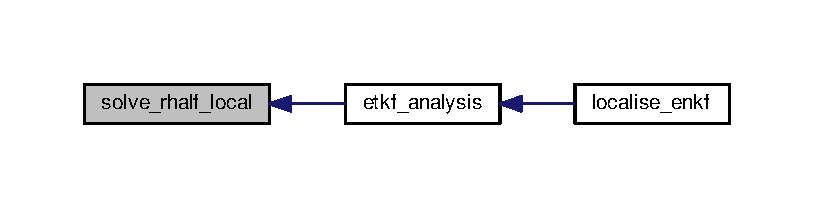
\includegraphics[width=350pt]{enkf__specific_8f90_a391c05218787eeebf53b181156e4fcde_icgraph}
\end{center}
\end{figure}



\hypertarget{equivalent__weights__step_8f90}{\section{src/filters/equivalent\-\_\-weights\-\_\-step.f90 File Reference}
\label{equivalent__weights__step_8f90}\index{src/filters/equivalent\-\_\-weights\-\_\-step.\-f90@{src/filters/equivalent\-\_\-weights\-\_\-step.\-f90}}
}
\subsection*{Functions/\-Subroutines}
\begin{DoxyCompactItemize}
\item 
subroutine \hyperlink{equivalent__weights__step_8f90_a3439a2d355440c40666f773e889e5f26}{equal\-\_\-weight\-\_\-filter}
\begin{DoxyCompactList}\small\item\em subroutine to do the equivalent weights step \end{DoxyCompactList}\end{DoxyCompactItemize}


\subsection{Function/\-Subroutine Documentation}
\hypertarget{equivalent__weights__step_8f90_a3439a2d355440c40666f773e889e5f26}{\index{equivalent\-\_\-weights\-\_\-step.\-f90@{equivalent\-\_\-weights\-\_\-step.\-f90}!equal\-\_\-weight\-\_\-filter@{equal\-\_\-weight\-\_\-filter}}
\index{equal\-\_\-weight\-\_\-filter@{equal\-\_\-weight\-\_\-filter}!equivalent_weights_step.f90@{equivalent\-\_\-weights\-\_\-step.\-f90}}
\subsubsection[{equal\-\_\-weight\-\_\-filter}]{\setlength{\rightskip}{0pt plus 5cm}subroutine equal\-\_\-weight\-\_\-filter (
\begin{DoxyParamCaption}
{}
\end{DoxyParamCaption}
)}}\label{equivalent__weights__step_8f90_a3439a2d355440c40666f773e889e5f26}


subroutine to do the equivalent weights step 



Here is the call graph for this function\-:\nopagebreak
\begin{figure}[H]
\begin{center}
\leavevmode
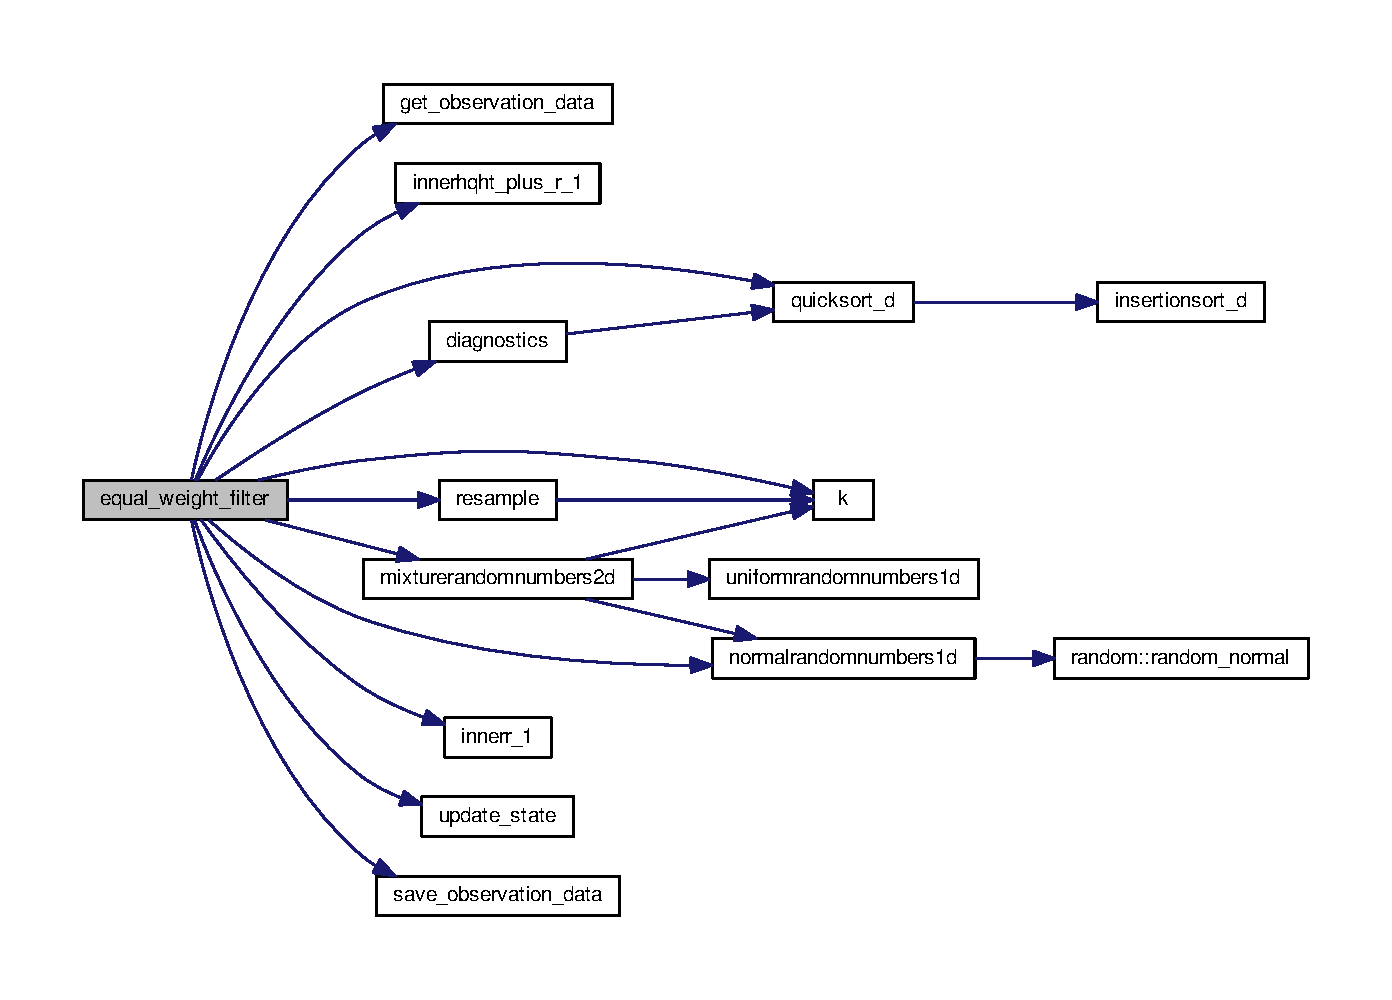
\includegraphics[width=350pt]{equivalent__weights__step_8f90_a3439a2d355440c40666f773e889e5f26_cgraph}
\end{center}
\end{figure}




Here is the caller graph for this function\-:\nopagebreak
\begin{figure}[H]
\begin{center}
\leavevmode
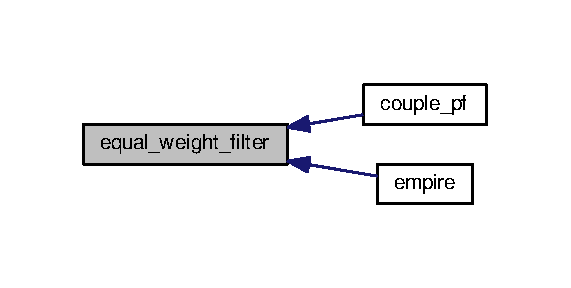
\includegraphics[width=274pt]{equivalent__weights__step_8f90_a3439a2d355440c40666f773e889e5f26_icgraph}
\end{center}
\end{figure}



\hypertarget{etkf__analysis_8f90}{\section{src/filters/etkf\-\_\-analysis.f90 File Reference}
\label{etkf__analysis_8f90}\index{src/filters/etkf\-\_\-analysis.\-f90@{src/filters/etkf\-\_\-analysis.\-f90}}
}
\subsection*{Functions/\-Subroutines}
\begin{DoxyCompactItemize}
\item 
subroutine \hyperlink{etkf__analysis_8f90_a7a1f0166706aef6167aad6525c792f66}{etkf\-\_\-analysis} (num\-\_\-hor, num\-\_\-ver, this\-\_\-hor, this\-\_\-ver, boundary, x, N, state\-Dim, obs\-Dim, rho)
\end{DoxyCompactItemize}


\subsection{Function/\-Subroutine Documentation}
\hypertarget{etkf__analysis_8f90_a7a1f0166706aef6167aad6525c792f66}{\index{etkf\-\_\-analysis.\-f90@{etkf\-\_\-analysis.\-f90}!etkf\-\_\-analysis@{etkf\-\_\-analysis}}
\index{etkf\-\_\-analysis@{etkf\-\_\-analysis}!etkf_analysis.f90@{etkf\-\_\-analysis.\-f90}}
\subsubsection[{etkf\-\_\-analysis}]{\setlength{\rightskip}{0pt plus 5cm}subroutine etkf\-\_\-analysis (
\begin{DoxyParamCaption}
\item[{integer, intent(in)}]{num\-\_\-hor, }
\item[{integer, intent(in)}]{num\-\_\-ver, }
\item[{integer, intent(in)}]{this\-\_\-hor, }
\item[{integer, intent(in)}]{this\-\_\-ver, }
\item[{integer, intent(in)}]{boundary, }
\item[{real(kind=rk), dimension(statedim,n), intent(inout)}]{x, }
\item[{integer, intent(in)}]{N, }
\item[{integer, intent(in)}]{state\-Dim, }
\item[{integer, intent(in)}]{obs\-Dim, }
\item[{real(kind=rk), intent(in)}]{rho}
\end{DoxyParamCaption}
)}}\label{etkf__analysis_8f90_a7a1f0166706aef6167aad6525c792f66}


Here is the call graph for this function\-:\nopagebreak
\begin{figure}[H]
\begin{center}
\leavevmode
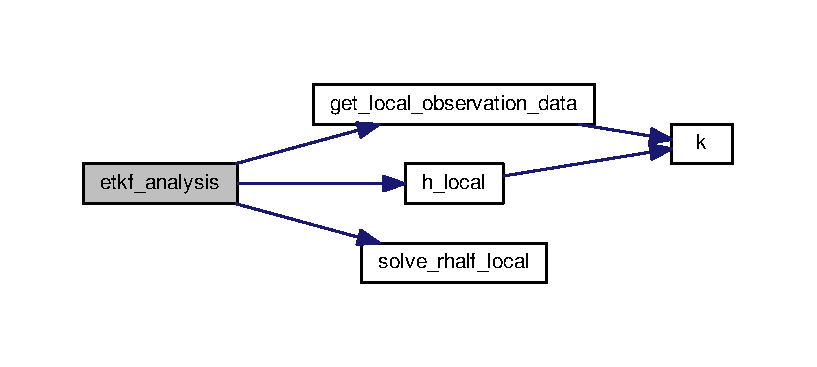
\includegraphics[width=350pt]{etkf__analysis_8f90_a7a1f0166706aef6167aad6525c792f66_cgraph}
\end{center}
\end{figure}




Here is the caller graph for this function\-:\nopagebreak
\begin{figure}[H]
\begin{center}
\leavevmode
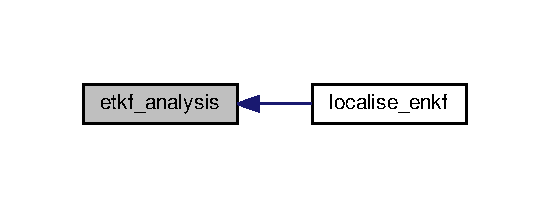
\includegraphics[width=264pt]{etkf__analysis_8f90_a7a1f0166706aef6167aad6525c792f66_icgraph}
\end{center}
\end{figure}



\hypertarget{proposal__filter_8f90}{\section{src/filters/proposal\-\_\-filter.f90 File Reference}
\label{proposal__filter_8f90}\index{src/filters/proposal\-\_\-filter.\-f90@{src/filters/proposal\-\_\-filter.\-f90}}
}
\subsection*{Functions/\-Subroutines}
\begin{DoxyCompactItemize}
\item 
subroutine \hyperlink{proposal__filter_8f90_ab8ccc692868eb53be1865567e85cb0b9}{proposal\-\_\-filter}
\begin{DoxyCompactList}\small\item\em Subroutine to perform nudging in the proposal step of E\-W\-P\-F. \end{DoxyCompactList}\end{DoxyCompactItemize}


\subsection{Function/\-Subroutine Documentation}
\hypertarget{proposal__filter_8f90_ab8ccc692868eb53be1865567e85cb0b9}{\index{proposal\-\_\-filter.\-f90@{proposal\-\_\-filter.\-f90}!proposal\-\_\-filter@{proposal\-\_\-filter}}
\index{proposal\-\_\-filter@{proposal\-\_\-filter}!proposal_filter.f90@{proposal\-\_\-filter.\-f90}}
\subsubsection[{proposal\-\_\-filter}]{\setlength{\rightskip}{0pt plus 5cm}subroutine proposal\-\_\-filter (
\begin{DoxyParamCaption}
{}
\end{DoxyParamCaption}
)}}\label{proposal__filter_8f90_ab8ccc692868eb53be1865567e85cb0b9}


Subroutine to perform nudging in the proposal step of E\-W\-P\-F. 



Here is the call graph for this function\-:\nopagebreak
\begin{figure}[H]
\begin{center}
\leavevmode
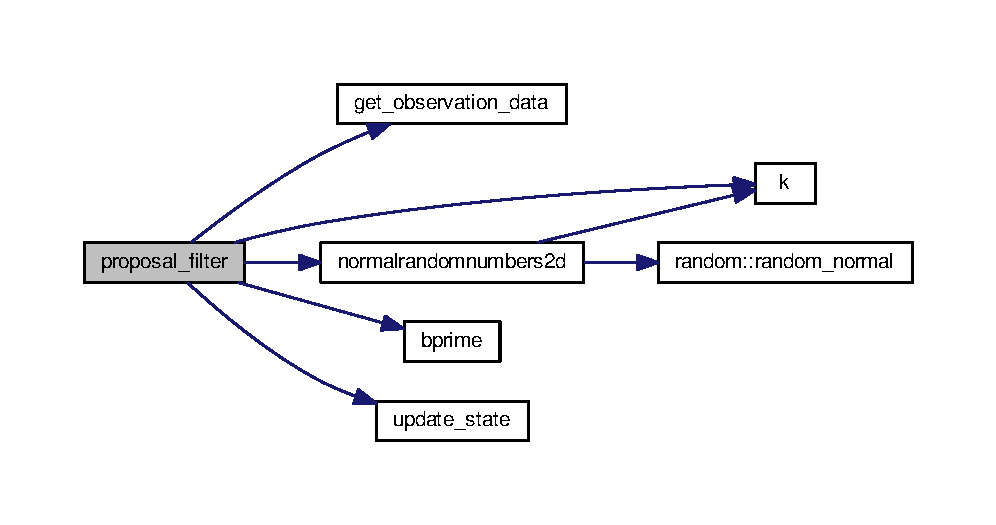
\includegraphics[width=350pt]{proposal__filter_8f90_ab8ccc692868eb53be1865567e85cb0b9_cgraph}
\end{center}
\end{figure}




Here is the caller graph for this function\-:\nopagebreak
\begin{figure}[H]
\begin{center}
\leavevmode
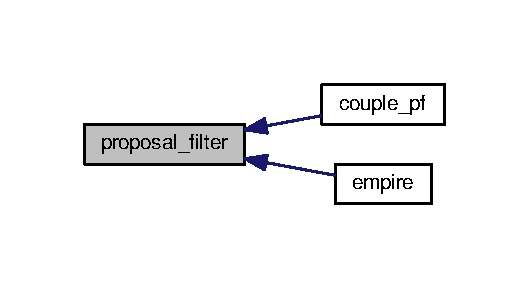
\includegraphics[width=254pt]{proposal__filter_8f90_ab8ccc692868eb53be1865567e85cb0b9_icgraph}
\end{center}
\end{figure}



\hypertarget{sir__filter_8f90}{\section{src/filters/sir\-\_\-filter.f90 File Reference}
\label{sir__filter_8f90}\index{src/filters/sir\-\_\-filter.\-f90@{src/filters/sir\-\_\-filter.\-f90}}
}
\subsection*{Functions/\-Subroutines}
\begin{DoxyCompactItemize}
\item 
subroutine \hyperlink{sir__filter_8f90_a856cc90b3cda652008e75f43e21297b8}{sir\-\_\-filter}
\begin{DoxyCompactList}\small\item\em Subroutine to perform S\-I\-R filter (Sequential Importance Resampling) \end{DoxyCompactList}\end{DoxyCompactItemize}


\subsection{Function/\-Subroutine Documentation}
\hypertarget{sir__filter_8f90_a856cc90b3cda652008e75f43e21297b8}{\index{sir\-\_\-filter.\-f90@{sir\-\_\-filter.\-f90}!sir\-\_\-filter@{sir\-\_\-filter}}
\index{sir\-\_\-filter@{sir\-\_\-filter}!sir_filter.f90@{sir\-\_\-filter.\-f90}}
\subsubsection[{sir\-\_\-filter}]{\setlength{\rightskip}{0pt plus 5cm}subroutine sir\-\_\-filter (
\begin{DoxyParamCaption}
{}
\end{DoxyParamCaption}
)}}\label{sir__filter_8f90_a856cc90b3cda652008e75f43e21297b8}


Subroutine to perform S\-I\-R filter (Sequential Importance Resampling) 



Here is the call graph for this function\-:\nopagebreak
\begin{figure}[H]
\begin{center}
\leavevmode
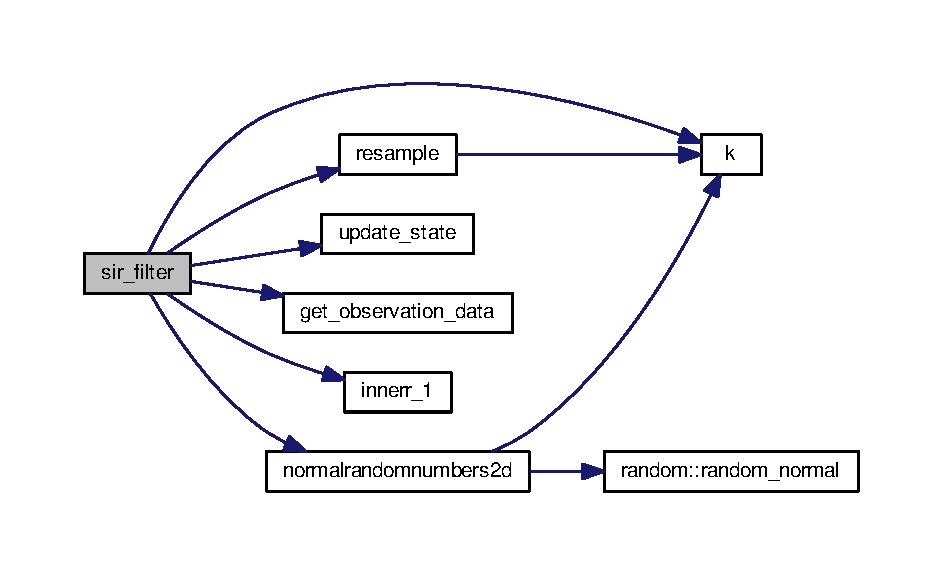
\includegraphics[width=350pt]{sir__filter_8f90_a856cc90b3cda652008e75f43e21297b8_cgraph}
\end{center}
\end{figure}




Here is the caller graph for this function\-:\nopagebreak
\begin{figure}[H]
\begin{center}
\leavevmode
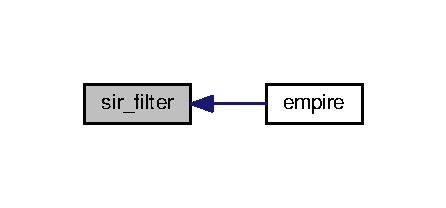
\includegraphics[width=214pt]{sir__filter_8f90_a856cc90b3cda652008e75f43e21297b8_icgraph}
\end{center}
\end{figure}



\hypertarget{stochastic__model_8f90}{\section{src/filters/stochastic\-\_\-model.f90 File Reference}
\label{stochastic__model_8f90}\index{src/filters/stochastic\-\_\-model.\-f90@{src/filters/stochastic\-\_\-model.\-f90}}
}
\subsection*{Functions/\-Subroutines}
\begin{DoxyCompactItemize}
\item 
subroutine \hyperlink{stochastic__model_8f90_ac824cdcc59bee27acef82df04a13e009}{stochastic\-\_\-model}
\begin{DoxyCompactList}\small\item\em subroutine to simply move the model forward in time one timestep P\-A\-B 21-\/05-\/2013 \end{DoxyCompactList}\item 
subroutine \hyperlink{stochastic__model_8f90_ae9b3f95267714a4c3991f2a1e6f85ded}{check\-\_\-scaling} (x, fx, b, scales)
\end{DoxyCompactItemize}


\subsection{Function/\-Subroutine Documentation}
\hypertarget{stochastic__model_8f90_ae9b3f95267714a4c3991f2a1e6f85ded}{\index{stochastic\-\_\-model.\-f90@{stochastic\-\_\-model.\-f90}!check\-\_\-scaling@{check\-\_\-scaling}}
\index{check\-\_\-scaling@{check\-\_\-scaling}!stochastic_model.f90@{stochastic\-\_\-model.\-f90}}
\subsubsection[{check\-\_\-scaling}]{\setlength{\rightskip}{0pt plus 5cm}subroutine check\-\_\-scaling (
\begin{DoxyParamCaption}
\item[{real(kind=rk), dimension(state\-\_\-dim), intent(in)}]{x, }
\item[{real(kind=rk), dimension(state\-\_\-dim), intent(in)}]{fx, }
\item[{real(kind=rk), dimension(state\-\_\-dim), intent(in)}]{b, }
\item[{real(kind=rk), dimension(9), intent(inout)}]{scales}
\end{DoxyParamCaption}
)}}\label{stochastic__model_8f90_ae9b3f95267714a4c3991f2a1e6f85ded}
\hypertarget{stochastic__model_8f90_ac824cdcc59bee27acef82df04a13e009}{\index{stochastic\-\_\-model.\-f90@{stochastic\-\_\-model.\-f90}!stochastic\-\_\-model@{stochastic\-\_\-model}}
\index{stochastic\-\_\-model@{stochastic\-\_\-model}!stochastic_model.f90@{stochastic\-\_\-model.\-f90}}
\subsubsection[{stochastic\-\_\-model}]{\setlength{\rightskip}{0pt plus 5cm}subroutine stochastic\-\_\-model (
\begin{DoxyParamCaption}
{}
\end{DoxyParamCaption}
)}}\label{stochastic__model_8f90_ac824cdcc59bee27acef82df04a13e009}


subroutine to simply move the model forward in time one timestep P\-A\-B 21-\/05-\/2013 



Here is the call graph for this function\-:\nopagebreak
\begin{figure}[H]
\begin{center}
\leavevmode
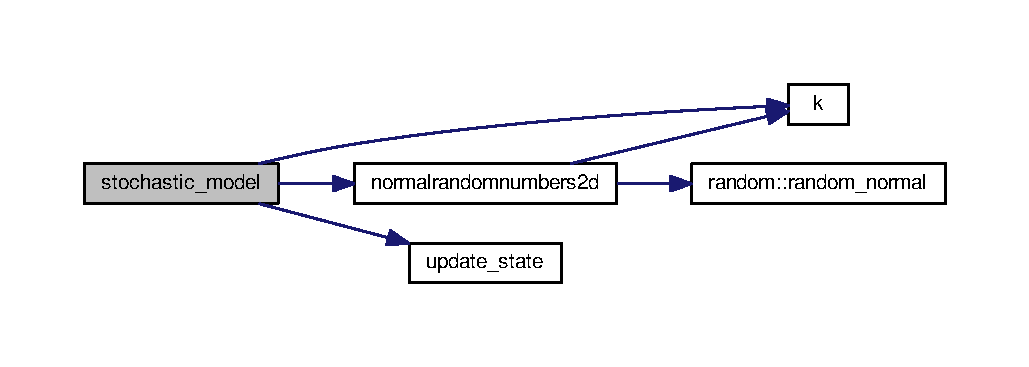
\includegraphics[width=350pt]{stochastic__model_8f90_ac824cdcc59bee27acef82df04a13e009_cgraph}
\end{center}
\end{figure}




Here is the caller graph for this function\-:\nopagebreak
\begin{figure}[H]
\begin{center}
\leavevmode
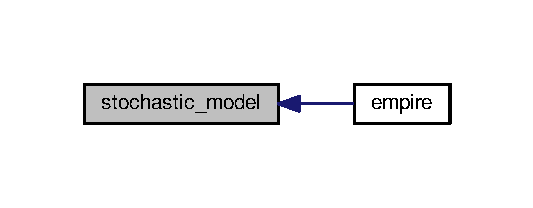
\includegraphics[width=256pt]{stochastic__model_8f90_ac824cdcc59bee27acef82df04a13e009_icgraph}
\end{center}
\end{figure}



\hypertarget{gen__rand_8f90}{\section{src/operations/gen\-\_\-rand.f90 File Reference}
\label{gen__rand_8f90}\index{src/operations/gen\-\_\-rand.\-f90@{src/operations/gen\-\_\-rand.\-f90}}
}
\subsection*{Functions/\-Subroutines}
\begin{DoxyCompactItemize}
\item 
subroutine \hyperlink{gen__rand_8f90_a7cd2e26a4fde81c03cf831511d512bd9}{uniformrandomnumbers1d} (minv, maxv, n, phi)
\begin{DoxyCompactList}\small\item\em generate one dimension of uniform random numbers \end{DoxyCompactList}\item 
subroutine \hyperlink{gen__rand_8f90_a009e8ce631181191ef16c1f99f43a158}{normalrandomnumbers1d} (mean, stdev, n, phi)
\begin{DoxyCompactList}\small\item\em generate one dimension of Normal random numbers \end{DoxyCompactList}\item 
subroutine \hyperlink{gen__rand_8f90_a79c7f64e458a6af30a2fa95a1650c917}{normalrandomnumbers2d} (mean, stdev, n, \hyperlink{operator__wrappers_8f90_aec571ade653c1cf8fd6cde17285af055}{k}, phi)
\begin{DoxyCompactList}\small\item\em generate two dimensional Normal random numbers \end{DoxyCompactList}\item 
subroutine \hyperlink{gen__rand_8f90_ad4c0e9c0f916eb9c4f784239c2768851}{mixturerandomnumbers1d} (mean, stdev, ufac, epsi, n, phi, uniform)
\begin{DoxyCompactList}\small\item\em generate one dimensional vector drawn from mixture density \end{DoxyCompactList}\item 
subroutine \hyperlink{gen__rand_8f90_a5ee81ac6968037e88d3686f9b477b77d}{mixturerandomnumbers2d} (mean, stdev, ufac, epsi, n, \hyperlink{operator__wrappers_8f90_aec571ade653c1cf8fd6cde17285af055}{k}, phi, uniform)
\begin{DoxyCompactList}\small\item\em generate two dimensional vector, each drawn from mixture density \end{DoxyCompactList}\item 
subroutine \hyperlink{gen__rand_8f90_ae9c8b02eca8aa840a34882d0836bcfff}{random\-\_\-seed\-\_\-mpi} (pfid)
\begin{DoxyCompactList}\small\item\em Subroutine to set the random seed across M\-P\-I threads. \end{DoxyCompactList}\end{DoxyCompactItemize}


\subsection{Function/\-Subroutine Documentation}
\hypertarget{gen__rand_8f90_ad4c0e9c0f916eb9c4f784239c2768851}{\index{gen\-\_\-rand.\-f90@{gen\-\_\-rand.\-f90}!mixturerandomnumbers1d@{mixturerandomnumbers1d}}
\index{mixturerandomnumbers1d@{mixturerandomnumbers1d}!gen_rand.f90@{gen\-\_\-rand.\-f90}}
\subsubsection[{mixturerandomnumbers1d}]{\setlength{\rightskip}{0pt plus 5cm}subroutine mixturerandomnumbers1d (
\begin{DoxyParamCaption}
\item[{real(kind=kind(1.\-0d0)), intent(in)}]{mean, }
\item[{real(kind=kind(1.\-0d0)), intent(in)}]{stdev, }
\item[{real(kind=kind(1.\-0d0)), intent(in)}]{ufac, }
\item[{real(kind=kind(1.\-0d0)), intent(in)}]{epsi, }
\item[{integer, intent(in)}]{n, }
\item[{real(kind=kind(1.\-0d0)), dimension(n), intent(out)}]{phi, }
\item[{logical, intent(out)}]{uniform}
\end{DoxyParamCaption}
)}}\label{gen__rand_8f90_ad4c0e9c0f916eb9c4f784239c2768851}


generate one dimensional vector drawn from mixture density 


\begin{DoxyParams}[1]{Parameters}
\mbox{\tt in}  & {\em mean} & Mean of normal distribution \\
\hline
\mbox{\tt in}  & {\em stdev} & Standard deviation of normal distribution \\
\hline
\mbox{\tt in}  & {\em ufac} & half-\/width of uniform distribution that is centered on the mean \\
\hline
\mbox{\tt in}  & {\em epsi} & Proportion controlling mixture draw. if random\-\_\-number $>$ epsi then draw from uniform, else normal \\
\hline
\mbox{\tt in}  & {\em n} & size of output vector \\
\hline
\mbox{\tt out}  & {\em phi} & n dimensional mixture random numbers \\
\hline
\mbox{\tt out}  & {\em uniform} & True if mixture drawn from uniform. False if drawn from normal \\
\hline
\end{DoxyParams}


Here is the call graph for this function\-:\nopagebreak
\begin{figure}[H]
\begin{center}
\leavevmode
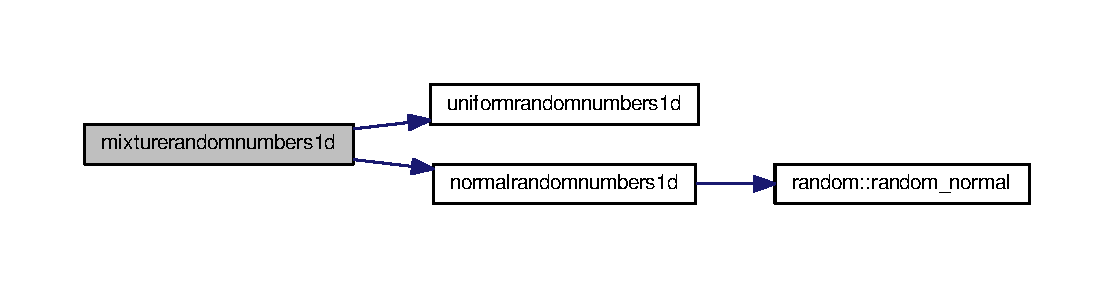
\includegraphics[width=350pt]{gen__rand_8f90_ad4c0e9c0f916eb9c4f784239c2768851_cgraph}
\end{center}
\end{figure}


\hypertarget{gen__rand_8f90_a5ee81ac6968037e88d3686f9b477b77d}{\index{gen\-\_\-rand.\-f90@{gen\-\_\-rand.\-f90}!mixturerandomnumbers2d@{mixturerandomnumbers2d}}
\index{mixturerandomnumbers2d@{mixturerandomnumbers2d}!gen_rand.f90@{gen\-\_\-rand.\-f90}}
\subsubsection[{mixturerandomnumbers2d}]{\setlength{\rightskip}{0pt plus 5cm}subroutine mixturerandomnumbers2d (
\begin{DoxyParamCaption}
\item[{real(kind=kind(1.\-0d0)), intent(in)}]{mean, }
\item[{real(kind=kind(1.\-0d0)), intent(in)}]{stdev, }
\item[{real(kind=kind(1.\-0d0)), intent(in)}]{ufac, }
\item[{real(kind=kind(1.\-0d0)), intent(in)}]{epsi, }
\item[{integer, intent(in)}]{n, }
\item[{integer, intent(in)}]{k, }
\item[{real(kind=kind(1.\-0d0)), dimension(n,k), intent(out)}]{phi, }
\item[{logical, dimension({\bf k}), intent(out)}]{uniform}
\end{DoxyParamCaption}
)}}\label{gen__rand_8f90_a5ee81ac6968037e88d3686f9b477b77d}


generate two dimensional vector, each drawn from mixture density 


\begin{DoxyParams}[1]{Parameters}
\mbox{\tt in}  & {\em mean} & Mean of normal distribution \\
\hline
\mbox{\tt in}  & {\em stdev} & Standard deviation of normal distribution \\
\hline
\mbox{\tt in}  & {\em ufac} & half-\/width of uniform distribution that is centered on the mean \\
\hline
\mbox{\tt in}  & {\em epsi} & Proportion controlling mixture draw. if random\-\_\-number $>$ epsi then draw from uniform, else normal \\
\hline
\mbox{\tt in}  & {\em n} & first dimension of output vector \\
\hline
\mbox{\tt in}  & {\em n} & second dimension of output vector \\
\hline
\mbox{\tt out}  & {\em phi} & n,k dimensional mixture random numbers \\
\hline
\mbox{\tt out}  & {\em uniform} & k dimensional logical with uniform(i) True if phi(\-:,i) drawn from uniform. False if drawn from normal \\
\hline
\end{DoxyParams}


Here is the call graph for this function\-:\nopagebreak
\begin{figure}[H]
\begin{center}
\leavevmode
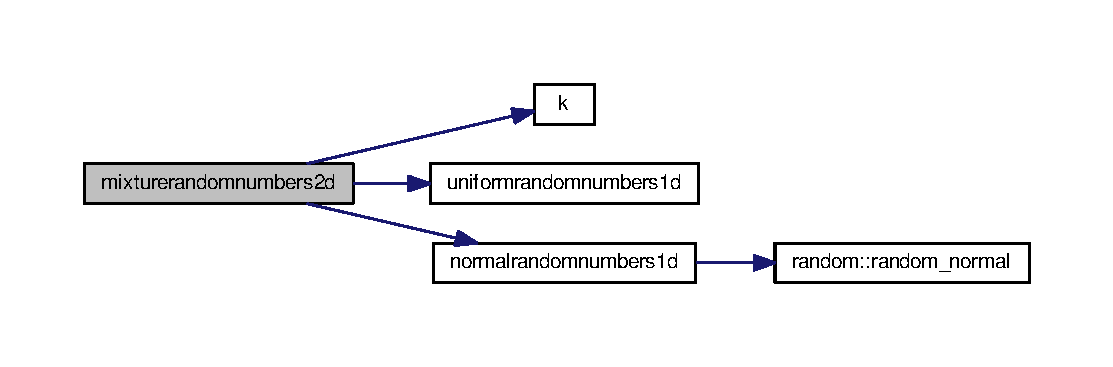
\includegraphics[width=350pt]{gen__rand_8f90_a5ee81ac6968037e88d3686f9b477b77d_cgraph}
\end{center}
\end{figure}




Here is the caller graph for this function\-:\nopagebreak
\begin{figure}[H]
\begin{center}
\leavevmode
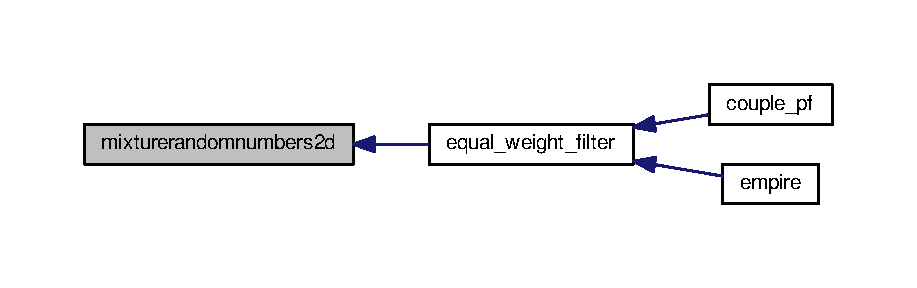
\includegraphics[width=350pt]{gen__rand_8f90_a5ee81ac6968037e88d3686f9b477b77d_icgraph}
\end{center}
\end{figure}


\hypertarget{gen__rand_8f90_a009e8ce631181191ef16c1f99f43a158}{\index{gen\-\_\-rand.\-f90@{gen\-\_\-rand.\-f90}!normalrandomnumbers1d@{normalrandomnumbers1d}}
\index{normalrandomnumbers1d@{normalrandomnumbers1d}!gen_rand.f90@{gen\-\_\-rand.\-f90}}
\subsubsection[{normalrandomnumbers1d}]{\setlength{\rightskip}{0pt plus 5cm}subroutine normalrandomnumbers1d (
\begin{DoxyParamCaption}
\item[{real(kind=rk), intent(in)}]{mean, }
\item[{real(kind=rk), intent(in)}]{stdev, }
\item[{integer, intent(in)}]{n, }
\item[{real(kind=rk), dimension(n), intent(out)}]{phi}
\end{DoxyParamCaption}
)}}\label{gen__rand_8f90_a009e8ce631181191ef16c1f99f43a158}


generate one dimension of Normal random numbers 


\begin{DoxyParams}[1]{Parameters}
\mbox{\tt in}  & {\em n} & size of output vector\\
\hline
\mbox{\tt in}  & {\em mean} & mean of normal distribution\\
\hline
\mbox{\tt in}  & {\em stdev} & Standard Deviation of normal distribution\\
\hline
\mbox{\tt out}  & {\em phi} & n dimensional normal random numbers \\
\hline
\end{DoxyParams}


Here is the call graph for this function\-:\nopagebreak
\begin{figure}[H]
\begin{center}
\leavevmode
\includegraphics[width=350pt]{gen__rand_8f90_a009e8ce631181191ef16c1f99f43a158_cgraph}
\end{center}
\end{figure}




Here is the caller graph for this function\-:\nopagebreak
\begin{figure}[H]
\begin{center}
\leavevmode
\includegraphics[width=350pt]{gen__rand_8f90_a009e8ce631181191ef16c1f99f43a158_icgraph}
\end{center}
\end{figure}


\hypertarget{gen__rand_8f90_a79c7f64e458a6af30a2fa95a1650c917}{\index{gen\-\_\-rand.\-f90@{gen\-\_\-rand.\-f90}!normalrandomnumbers2d@{normalrandomnumbers2d}}
\index{normalrandomnumbers2d@{normalrandomnumbers2d}!gen_rand.f90@{gen\-\_\-rand.\-f90}}
\subsubsection[{normalrandomnumbers2d}]{\setlength{\rightskip}{0pt plus 5cm}subroutine normalrandomnumbers2d (
\begin{DoxyParamCaption}
\item[{real(kind=rk), intent(in)}]{mean, }
\item[{real(kind=rk), intent(in)}]{stdev, }
\item[{integer, intent(in)}]{n, }
\item[{integer, intent(in)}]{k, }
\item[{real(kind=rk), dimension(n,{\bf k}), intent(out)}]{phi}
\end{DoxyParamCaption}
)}}\label{gen__rand_8f90_a79c7f64e458a6af30a2fa95a1650c917}


generate two dimensional Normal random numbers 


\begin{DoxyParams}[1]{Parameters}
\mbox{\tt in}  & {\em n} & first dimension of output vector\\
\hline
\mbox{\tt in}  & {\em n} & second dimension of output vector\\
\hline
\mbox{\tt in}  & {\em mean} & mean of normal distribution\\
\hline
\mbox{\tt in}  & {\em stdev} & Standard Deviation of normal distribution\\
\hline
\mbox{\tt out}  & {\em phi} & n,k dimensional normal random numbers \\
\hline
\end{DoxyParams}


Here is the call graph for this function\-:\nopagebreak
\begin{figure}[H]
\begin{center}
\leavevmode
\includegraphics[width=350pt]{gen__rand_8f90_a79c7f64e458a6af30a2fa95a1650c917_cgraph}
\end{center}
\end{figure}




Here is the caller graph for this function\-:\nopagebreak
\begin{figure}[H]
\begin{center}
\leavevmode
\includegraphics[width=350pt]{gen__rand_8f90_a79c7f64e458a6af30a2fa95a1650c917_icgraph}
\end{center}
\end{figure}


\hypertarget{gen__rand_8f90_ae9c8b02eca8aa840a34882d0836bcfff}{\index{gen\-\_\-rand.\-f90@{gen\-\_\-rand.\-f90}!random\-\_\-seed\-\_\-mpi@{random\-\_\-seed\-\_\-mpi}}
\index{random\-\_\-seed\-\_\-mpi@{random\-\_\-seed\-\_\-mpi}!gen_rand.f90@{gen\-\_\-rand.\-f90}}
\subsubsection[{random\-\_\-seed\-\_\-mpi}]{\setlength{\rightskip}{0pt plus 5cm}subroutine random\-\_\-seed\-\_\-mpi (
\begin{DoxyParamCaption}
\item[{integer, intent(in)}]{pfid}
\end{DoxyParamCaption}
)}}\label{gen__rand_8f90_ae9c8b02eca8aa840a34882d0836bcfff}


Subroutine to set the random seed across M\-P\-I threads. 


\begin{DoxyParams}[1]{Parameters}
\mbox{\tt in}  & {\em pfid} & The process identifier of the M\-P\-I process \\
\hline
\end{DoxyParams}


Here is the caller graph for this function\-:\nopagebreak
\begin{figure}[H]
\begin{center}
\leavevmode
\includegraphics[width=272pt]{gen__rand_8f90_ae9c8b02eca8aa840a34882d0836bcfff_icgraph}
\end{center}
\end{figure}


\hypertarget{gen__rand_8f90_a7cd2e26a4fde81c03cf831511d512bd9}{\index{gen\-\_\-rand.\-f90@{gen\-\_\-rand.\-f90}!uniformrandomnumbers1d@{uniformrandomnumbers1d}}
\index{uniformrandomnumbers1d@{uniformrandomnumbers1d}!gen_rand.f90@{gen\-\_\-rand.\-f90}}
\subsubsection[{uniformrandomnumbers1d}]{\setlength{\rightskip}{0pt plus 5cm}subroutine uniformrandomnumbers1d (
\begin{DoxyParamCaption}
\item[{real(kind=rk), intent(in)}]{minv, }
\item[{real(kind=rk), intent(in)}]{maxv, }
\item[{integer, intent(in)}]{n, }
\item[{real(kind=rk), dimension(n), intent(out)}]{phi}
\end{DoxyParamCaption}
)}}\label{gen__rand_8f90_a7cd2e26a4fde81c03cf831511d512bd9}


generate one dimension of uniform random numbers 


\begin{DoxyParams}[1]{Parameters}
\mbox{\tt in}  & {\em n} & size of output vector\\
\hline
\mbox{\tt in}  & {\em minv} & minimum value of uniform distribution\\
\hline
\mbox{\tt in}  & {\em maxv} & maximum value of uniform distribution\\
\hline
\mbox{\tt out}  & {\em phi} & n dimensional uniform random numbers \\
\hline
\end{DoxyParams}


Here is the caller graph for this function\-:\nopagebreak
\begin{figure}[H]
\begin{center}
\leavevmode
\includegraphics[width=350pt]{gen__rand_8f90_a7cd2e26a4fde81c03cf831511d512bd9_icgraph}
\end{center}
\end{figure}



\hypertarget{operator__wrappers_8f90}{\section{src/operations/operator\-\_\-wrappers.f90 File Reference}
\label{operator__wrappers_8f90}\index{src/operations/operator\-\_\-wrappers.\-f90@{src/operations/operator\-\_\-wrappers.\-f90}}
}
\subsection*{Functions/\-Subroutines}
\begin{DoxyCompactItemize}
\item 
subroutine \hyperlink{operator__wrappers_8f90_aec571ade653c1cf8fd6cde17285af055}{k} (y, x)
\begin{DoxyCompactList}\small\item\em Subroutine to apply $K$ to a vector y in observation space where $K := QH^T(HQH^T+R)^{-1}$. \end{DoxyCompactList}\item 
subroutine \hyperlink{operator__wrappers_8f90_adb7f01ab90a983549eaf0ebb1f5c8289}{innerr\-\_\-1} (y, w)
\begin{DoxyCompactList}\small\item\em subroutine to compute the inner product with $R^{-1}$ \end{DoxyCompactList}\item 
subroutine \hyperlink{operator__wrappers_8f90_a2bdcf5ca1fde3d87061ae8e984b4c1d9}{innerhqht\-\_\-plus\-\_\-r\-\_\-1} (y, w)
\begin{DoxyCompactList}\small\item\em subroutine to compute the inner product with $(HQH^T+R)^{-1}$ \end{DoxyCompactList}\item 
subroutine \hyperlink{operator__wrappers_8f90_a96d0c9700917cd1bcb959b2d96e27036}{bprime} (y, x, Q\-Ht\-R\-\_\-1y, normaln, betan)
\begin{DoxyCompactList}\small\item\em subroutine to calculate nudging term and correlated random errors efficiently \end{DoxyCompactList}\end{DoxyCompactItemize}


\subsection{Function/\-Subroutine Documentation}
\hypertarget{operator__wrappers_8f90_a96d0c9700917cd1bcb959b2d96e27036}{\index{operator\-\_\-wrappers.\-f90@{operator\-\_\-wrappers.\-f90}!bprime@{bprime}}
\index{bprime@{bprime}!operator_wrappers.f90@{operator\-\_\-wrappers.\-f90}}
\subsubsection[{bprime}]{\setlength{\rightskip}{0pt plus 5cm}subroutine bprime (
\begin{DoxyParamCaption}
\item[{real(kind=rk), dimension(obs\-\_\-dim,pf\%count), intent(in)}]{y, }
\item[{real(kind=rk), dimension(state\-\_\-dim,pf\%count), intent(out)}]{x, }
\item[{real(kind=rk), dimension(state\-\_\-dim,pf\%count), intent(out)}]{Q\-Ht\-R\-\_\-1y, }
\item[{real(kind=rk), dimension(state\-\_\-dim,pf\%count), intent(in)}]{normaln, }
\item[{real(kind=rk), dimension(state\-\_\-dim,pf\%count), intent(out)}]{betan}
\end{DoxyParamCaption}
)}}\label{operator__wrappers_8f90_a96d0c9700917cd1bcb959b2d96e27036}


subroutine to calculate nudging term and correlated random errors efficiently 


\begin{DoxyParams}[1]{Parameters}
\mbox{\tt in}  & {\em y} & (obs\-\_\-dim,pf\%count) vectors of innovations $y-H(x^{n-1})$ \\
\hline
\mbox{\tt out}  & {\em x} & (state\-\_\-dim,pf\%count) vectors of $\rho Q^{\frac{1}{2}}H^TR^{-1}[y-H(x^{n-1})]$ \\
\hline
\mbox{\tt out}  & {\em Q\-Ht\-R\-\_\-1y} & (state\-\_\-dim,pf\%count) vectors of $\rho QH^TR^{-1}[y-H(x^{n-1})]$ \\
\hline
\mbox{\tt in}  & {\em normaln} & (state\-\_\-dim,pf\%count) uncorrelated random vectors such that normaln(\-:,i) $\sim \mathcal{N}(0,I)$ \\
\hline
\mbox{\tt out}  & {\em betan} & (state\-\_\-dim,pf\%count) correlated random vectors such that betan(\-:,i) $\sim \mathcal{N}(0,Q)$ \\
\hline
\end{DoxyParams}


Here is the caller graph for this function\-:\nopagebreak
\begin{figure}[H]
\begin{center}
\leavevmode
\includegraphics[width=336pt]{operator__wrappers_8f90_a96d0c9700917cd1bcb959b2d96e27036_icgraph}
\end{center}
\end{figure}


\hypertarget{operator__wrappers_8f90_a2bdcf5ca1fde3d87061ae8e984b4c1d9}{\index{operator\-\_\-wrappers.\-f90@{operator\-\_\-wrappers.\-f90}!innerhqht\-\_\-plus\-\_\-r\-\_\-1@{innerhqht\-\_\-plus\-\_\-r\-\_\-1}}
\index{innerhqht\-\_\-plus\-\_\-r\-\_\-1@{innerhqht\-\_\-plus\-\_\-r\-\_\-1}!operator_wrappers.f90@{operator\-\_\-wrappers.\-f90}}
\subsubsection[{innerhqht\-\_\-plus\-\_\-r\-\_\-1}]{\setlength{\rightskip}{0pt plus 5cm}subroutine innerhqht\-\_\-plus\-\_\-r\-\_\-1 (
\begin{DoxyParamCaption}
\item[{real(kind=rk), dimension(obs\-\_\-dim), intent(in)}]{y, }
\item[{real(kind=rk), intent(out)}]{w}
\end{DoxyParamCaption}
)}}\label{operator__wrappers_8f90_a2bdcf5ca1fde3d87061ae8e984b4c1d9}


subroutine to compute the inner product with $(HQH^T+R)^{-1}$ 


\begin{DoxyParams}[1]{Parameters}
\mbox{\tt in}  & {\em y} & vector in observation space \\
\hline
\mbox{\tt out}  & {\em w} & scalar with value $y^TR^{-1}y$ \\
\hline
\end{DoxyParams}


Here is the caller graph for this function\-:\nopagebreak
\begin{figure}[H]
\begin{center}
\leavevmode
\includegraphics[width=350pt]{operator__wrappers_8f90_a2bdcf5ca1fde3d87061ae8e984b4c1d9_icgraph}
\end{center}
\end{figure}


\hypertarget{operator__wrappers_8f90_adb7f01ab90a983549eaf0ebb1f5c8289}{\index{operator\-\_\-wrappers.\-f90@{operator\-\_\-wrappers.\-f90}!innerr\-\_\-1@{innerr\-\_\-1}}
\index{innerr\-\_\-1@{innerr\-\_\-1}!operator_wrappers.f90@{operator\-\_\-wrappers.\-f90}}
\subsubsection[{innerr\-\_\-1}]{\setlength{\rightskip}{0pt plus 5cm}subroutine innerr\-\_\-1 (
\begin{DoxyParamCaption}
\item[{real(kind=rk), dimension(obs\-\_\-dim,pf\%count), intent(in)}]{y, }
\item[{real(kind=rk), dimension(pf\%count), intent(out)}]{w}
\end{DoxyParamCaption}
)}}\label{operator__wrappers_8f90_adb7f01ab90a983549eaf0ebb1f5c8289}


subroutine to compute the inner product with $R^{-1}$ 


\begin{DoxyParams}[1]{Parameters}
\mbox{\tt in}  & {\em y} & multiple vectors in observation space (pf\%count of them) \\
\hline
\mbox{\tt out}  & {\em w} & multiple scalars (pf\%count) where w(i) has the value $y(:,i)^TR^{-1}y(:,i)$ \\
\hline
\end{DoxyParams}


Here is the caller graph for this function\-:\nopagebreak
\begin{figure}[H]
\begin{center}
\leavevmode
\includegraphics[width=350pt]{operator__wrappers_8f90_adb7f01ab90a983549eaf0ebb1f5c8289_icgraph}
\end{center}
\end{figure}


\hypertarget{operator__wrappers_8f90_aec571ade653c1cf8fd6cde17285af055}{\index{operator\-\_\-wrappers.\-f90@{operator\-\_\-wrappers.\-f90}!k@{k}}
\index{k@{k}!operator_wrappers.f90@{operator\-\_\-wrappers.\-f90}}
\subsubsection[{k}]{\setlength{\rightskip}{0pt plus 5cm}subroutine k (
\begin{DoxyParamCaption}
\item[{real(kind=rk), dimension(obs\-\_\-dim,pf\%count), intent(in)}]{y, }
\item[{real(kind=rk), dimension(state\-\_\-dim,pf\%count), intent(out)}]{x}
\end{DoxyParamCaption}
)}}\label{operator__wrappers_8f90_aec571ade653c1cf8fd6cde17285af055}


Subroutine to apply $K$ to a vector y in observation space where $K := QH^T(HQH^T+R)^{-1}$. 


\begin{DoxyParams}[1]{Parameters}
\mbox{\tt in}  & {\em y} & vector in observation space \\
\hline
\mbox{\tt out}  & {\em x} & vector in state space \\
\hline
\end{DoxyParams}


Here is the caller graph for this function\-:\nopagebreak
\begin{figure}[H]
\begin{center}
\leavevmode
\includegraphics[height=550pt]{operator__wrappers_8f90_aec571ade653c1cf8fd6cde17285af055_icgraph}
\end{center}
\end{figure}



\hypertarget{perturb__particle_8f90}{\section{src/operations/perturb\-\_\-particle.f90 File Reference}
\label{perturb__particle_8f90}\index{src/operations/perturb\-\_\-particle.\-f90@{src/operations/perturb\-\_\-particle.\-f90}}
}
\subsection*{Functions/\-Subroutines}
\begin{DoxyCompactItemize}
\item 
subroutine \hyperlink{perturb__particle_8f90_a6948efec663affbf7e1b3877298ee9c9}{perturb\-\_\-particle} (x)
\begin{DoxyCompactList}\small\item\em Subroutine to perturb state vector with normal random vector drawn from $\mathcal{N}(0,Q)$. \end{DoxyCompactList}\item 
subroutine \hyperlink{perturb__particle_8f90_a7b7fb7c4adca778bebb88945eaa8e564}{update\-\_\-state} (state, fpsi, kgain, betan)
\begin{DoxyCompactList}\small\item\em Subroutine to update the state. \end{DoxyCompactList}\end{DoxyCompactItemize}


\subsection{Function/\-Subroutine Documentation}
\hypertarget{perturb__particle_8f90_a6948efec663affbf7e1b3877298ee9c9}{\index{perturb\-\_\-particle.\-f90@{perturb\-\_\-particle.\-f90}!perturb\-\_\-particle@{perturb\-\_\-particle}}
\index{perturb\-\_\-particle@{perturb\-\_\-particle}!perturb_particle.f90@{perturb\-\_\-particle.\-f90}}
\subsubsection[{perturb\-\_\-particle}]{\setlength{\rightskip}{0pt plus 5cm}subroutine perturb\-\_\-particle (
\begin{DoxyParamCaption}
\item[{real(kind=rk), dimension(state\-\_\-dim), intent(inout)}]{x}
\end{DoxyParamCaption}
)}}\label{perturb__particle_8f90_a6948efec663affbf7e1b3877298ee9c9}


Subroutine to perturb state vector with normal random vector drawn from $\mathcal{N}(0,Q)$. 



Here is the call graph for this function\-:\nopagebreak
\begin{figure}[H]
\begin{center}
\leavevmode
\includegraphics[width=350pt]{perturb__particle_8f90_a6948efec663affbf7e1b3877298ee9c9_cgraph}
\end{center}
\end{figure}




Here is the caller graph for this function\-:\nopagebreak
\begin{figure}[H]
\begin{center}
\leavevmode
\includegraphics[width=260pt]{perturb__particle_8f90_a6948efec663affbf7e1b3877298ee9c9_icgraph}
\end{center}
\end{figure}


\hypertarget{perturb__particle_8f90_a7b7fb7c4adca778bebb88945eaa8e564}{\index{perturb\-\_\-particle.\-f90@{perturb\-\_\-particle.\-f90}!update\-\_\-state@{update\-\_\-state}}
\index{update\-\_\-state@{update\-\_\-state}!perturb_particle.f90@{perturb\-\_\-particle.\-f90}}
\subsubsection[{update\-\_\-state}]{\setlength{\rightskip}{0pt plus 5cm}subroutine update\-\_\-state (
\begin{DoxyParamCaption}
\item[{real(kind=rk), dimension(state\-\_\-dim), intent(out)}]{state, }
\item[{real(kind=rk), dimension(state\-\_\-dim), intent(in)}]{fpsi, }
\item[{real(kind=rk), dimension(state\-\_\-dim), intent(in)}]{kgain, }
\item[{real(kind=rk), dimension(state\-\_\-dim), intent(inout)}]{betan}
\end{DoxyParamCaption}
)}}\label{perturb__particle_8f90_a7b7fb7c4adca778bebb88945eaa8e564}


Subroutine to update the state. 

This can be changed for the specific model if it needs to be


\begin{DoxyParams}[1]{Parameters}
\mbox{\tt in}  & {\em fpsi} & deterministic model update $f(x^{n-1})$ \\
\hline
\mbox{\tt in}  & {\em kgain} & nudging term \\
\hline
\mbox{\tt in,out}  & {\em betan} & Stochastic term \\
\hline
\mbox{\tt out}  & {\em state} & The updated state vector \\
\hline
\end{DoxyParams}


Here is the caller graph for this function\-:\nopagebreak
\begin{figure}[H]
\begin{center}
\leavevmode
\includegraphics[width=350pt]{perturb__particle_8f90_a7b7fb7c4adca778bebb88945eaa8e564_icgraph}
\end{center}
\end{figure}



\hypertarget{resample_8f90}{\section{src/operations/resample.f90 File Reference}
\label{resample_8f90}\index{src/operations/resample.\-f90@{src/operations/resample.\-f90}}
}
\subsection*{Functions/\-Subroutines}
\begin{DoxyCompactItemize}
\item 
subroutine \hyperlink{resample_8f90_ae311a90c08af18a1250ccc2087e7ff46}{resample}
\begin{DoxyCompactList}\small\item\em Subroutine to perform Universal Importance Resampling. \end{DoxyCompactList}\end{DoxyCompactItemize}


\subsection{Function/\-Subroutine Documentation}
\hypertarget{resample_8f90_ae311a90c08af18a1250ccc2087e7ff46}{\index{resample.\-f90@{resample.\-f90}!resample@{resample}}
\index{resample@{resample}!resample.f90@{resample.\-f90}}
\subsubsection[{resample}]{\setlength{\rightskip}{0pt plus 5cm}subroutine resample (
\begin{DoxyParamCaption}
{}
\end{DoxyParamCaption}
)}}\label{resample_8f90_ae311a90c08af18a1250ccc2087e7ff46}


Subroutine to perform Universal Importance Resampling. 



Here is the call graph for this function\-:\nopagebreak
\begin{figure}[H]
\begin{center}
\leavevmode
\includegraphics[width=202pt]{resample_8f90_ae311a90c08af18a1250ccc2087e7ff46_cgraph}
\end{center}
\end{figure}




Here is the caller graph for this function\-:\nopagebreak
\begin{figure}[H]
\begin{center}
\leavevmode
\includegraphics[width=350pt]{resample_8f90_ae311a90c08af18a1250ccc2087e7ff46_icgraph}
\end{center}
\end{figure}



\hypertarget{alltests_8f90}{\section{src/tests/alltests.f90 File Reference}
\label{alltests_8f90}\index{src/tests/alltests.\-f90@{src/tests/alltests.\-f90}}
}
\subsection*{Functions/\-Subroutines}
\begin{DoxyCompactItemize}
\item 
program \hyperlink{alltests_8f90_a153687a2c4fa8a55ff954238463e56ed}{alltests}
\begin{DoxyCompactList}\small\item\em program to run all tests of user specific functions \end{DoxyCompactList}\end{DoxyCompactItemize}


\subsection{Function/\-Subroutine Documentation}
\hypertarget{alltests_8f90_a153687a2c4fa8a55ff954238463e56ed}{\index{alltests.\-f90@{alltests.\-f90}!alltests@{alltests}}
\index{alltests@{alltests}!alltests.f90@{alltests.\-f90}}
\subsubsection[{alltests}]{\setlength{\rightskip}{0pt plus 5cm}program alltests (
\begin{DoxyParamCaption}
{}
\end{DoxyParamCaption}
)}}\label{alltests_8f90_a153687a2c4fa8a55ff954238463e56ed}


program to run all tests of user specific functions 



Here is the call graph for this function\-:\nopagebreak
\begin{figure}[H]
\begin{center}
\leavevmode
\includegraphics[width=350pt]{alltests_8f90_a153687a2c4fa8a55ff954238463e56ed_cgraph}
\end{center}
\end{figure}



\hypertarget{test__h_8f90}{\section{src/tests/test\-\_\-h.f90 File Reference}
\label{test__h_8f90}\index{src/tests/test\-\_\-h.\-f90@{src/tests/test\-\_\-h.\-f90}}
}
\subsection*{Functions/\-Subroutines}
\begin{DoxyCompactItemize}
\item 
program \hyperlink{test__h_8f90_a0f4f625f319b4dd6f5df8a572123e1de}{test\-\_\-h}
\begin{DoxyCompactList}\small\item\em program to run tests of user supplied observation operator \end{DoxyCompactList}\end{DoxyCompactItemize}


\subsection{Function/\-Subroutine Documentation}
\hypertarget{test__h_8f90_a0f4f625f319b4dd6f5df8a572123e1de}{\index{test\-\_\-h.\-f90@{test\-\_\-h.\-f90}!test\-\_\-h@{test\-\_\-h}}
\index{test\-\_\-h@{test\-\_\-h}!test_h.f90@{test\-\_\-h.\-f90}}
\subsubsection[{test\-\_\-h}]{\setlength{\rightskip}{0pt plus 5cm}program test\-\_\-h (
\begin{DoxyParamCaption}
{}
\end{DoxyParamCaption}
)}}\label{test__h_8f90_a0f4f625f319b4dd6f5df8a572123e1de}


program to run tests of user supplied observation operator 



Here is the call graph for this function\-:\nopagebreak
\begin{figure}[H]
\begin{center}
\leavevmode
\includegraphics[width=350pt]{test__h_8f90_a0f4f625f319b4dd6f5df8a572123e1de_cgraph}
\end{center}
\end{figure}



\hypertarget{test__hqhtr_8f90}{\section{src/tests/test\-\_\-hqhtr.f90 File Reference}
\label{test__hqhtr_8f90}\index{src/tests/test\-\_\-hqhtr.\-f90@{src/tests/test\-\_\-hqhtr.\-f90}}
}
\subsection*{Functions/\-Subroutines}
\begin{DoxyCompactItemize}
\item 
program \hyperlink{test__hqhtr_8f90_a64d8bb40fc118582dfad8ab274feebfd}{test\-\_\-hqhtr}
\begin{DoxyCompactList}\small\item\em program to run tests of user supplied linear solve \end{DoxyCompactList}\end{DoxyCompactItemize}


\subsection{Function/\-Subroutine Documentation}
\hypertarget{test__hqhtr_8f90_a64d8bb40fc118582dfad8ab274feebfd}{\index{test\-\_\-hqhtr.\-f90@{test\-\_\-hqhtr.\-f90}!test\-\_\-hqhtr@{test\-\_\-hqhtr}}
\index{test\-\_\-hqhtr@{test\-\_\-hqhtr}!test_hqhtr.f90@{test\-\_\-hqhtr.\-f90}}
\subsubsection[{test\-\_\-hqhtr}]{\setlength{\rightskip}{0pt plus 5cm}program test\-\_\-hqhtr (
\begin{DoxyParamCaption}
{}
\end{DoxyParamCaption}
)}}\label{test__hqhtr_8f90_a64d8bb40fc118582dfad8ab274feebfd}


program to run tests of user supplied linear solve 

$(HQH^T+R)^{-1}$ 

Here is the call graph for this function\-:\nopagebreak
\begin{figure}[H]
\begin{center}
\leavevmode
\includegraphics[width=350pt]{test__hqhtr_8f90_a64d8bb40fc118582dfad8ab274feebfd_cgraph}
\end{center}
\end{figure}



\hypertarget{test__q_8f90}{\section{src/tests/test\-\_\-q.f90 File Reference}
\label{test__q_8f90}\index{src/tests/test\-\_\-q.\-f90@{src/tests/test\-\_\-q.\-f90}}
}
\subsection*{Functions/\-Subroutines}
\begin{DoxyCompactItemize}
\item 
program \hyperlink{test__q_8f90_a8f31034aebc450c6e93cfe185f5ac347}{test\-\_\-q}
\begin{DoxyCompactList}\small\item\em program to run tests of user supplied model error covariance matrix \end{DoxyCompactList}\end{DoxyCompactItemize}


\subsection{Function/\-Subroutine Documentation}
\hypertarget{test__q_8f90_a8f31034aebc450c6e93cfe185f5ac347}{\index{test\-\_\-q.\-f90@{test\-\_\-q.\-f90}!test\-\_\-q@{test\-\_\-q}}
\index{test\-\_\-q@{test\-\_\-q}!test_q.f90@{test\-\_\-q.\-f90}}
\subsubsection[{test\-\_\-q}]{\setlength{\rightskip}{0pt plus 5cm}program test\-\_\-q (
\begin{DoxyParamCaption}
{}
\end{DoxyParamCaption}
)}}\label{test__q_8f90_a8f31034aebc450c6e93cfe185f5ac347}


program to run tests of user supplied model error covariance matrix 



Here is the call graph for this function\-:\nopagebreak
\begin{figure}[H]
\begin{center}
\leavevmode
\includegraphics[width=350pt]{test__q_8f90_a8f31034aebc450c6e93cfe185f5ac347_cgraph}
\end{center}
\end{figure}



\hypertarget{test__r_8f90}{\section{src/tests/test\-\_\-r.f90 File Reference}
\label{test__r_8f90}\index{src/tests/test\-\_\-r.\-f90@{src/tests/test\-\_\-r.\-f90}}
}
\subsection*{Functions/\-Subroutines}
\begin{DoxyCompactItemize}
\item 
program \hyperlink{test__r_8f90_ac6d09bf0961d83c56edf388b3162b347}{test\-\_\-r}
\begin{DoxyCompactList}\small\item\em program to run all tests of user supplied observation error covariance matrix/ \end{DoxyCompactList}\end{DoxyCompactItemize}


\subsection{Function/\-Subroutine Documentation}
\hypertarget{test__r_8f90_ac6d09bf0961d83c56edf388b3162b347}{\index{test\-\_\-r.\-f90@{test\-\_\-r.\-f90}!test\-\_\-r@{test\-\_\-r}}
\index{test\-\_\-r@{test\-\_\-r}!test_r.f90@{test\-\_\-r.\-f90}}
\subsubsection[{test\-\_\-r}]{\setlength{\rightskip}{0pt plus 5cm}program test\-\_\-r (
\begin{DoxyParamCaption}
{}
\end{DoxyParamCaption}
)}}\label{test__r_8f90_ac6d09bf0961d83c56edf388b3162b347}


program to run all tests of user supplied observation error covariance matrix/ 



Here is the call graph for this function\-:\nopagebreak
\begin{figure}[H]
\begin{center}
\leavevmode
\includegraphics[width=350pt]{test__r_8f90_ac6d09bf0961d83c56edf388b3162b347_cgraph}
\end{center}
\end{figure}



\hypertarget{tests_8f90}{\section{src/tests/tests.f90 File Reference}
\label{tests_8f90}\index{src/tests/tests.\-f90@{src/tests/tests.\-f90}}
}
\subsection*{Functions/\-Subroutines}
\begin{DoxyCompactItemize}
\item 
subroutine \hyperlink{tests_8f90_a3615a6c269d5a0f35a44f0801b4a921a}{h\-\_\-tests} ()
\item 
subroutine \hyperlink{tests_8f90_ae377b636e622fd3c952ed6190f3fdc18}{r\-\_\-tests} ()
\item 
subroutine \hyperlink{tests_8f90_ac15a5a85a2487c7489c22096a3c681e7}{q\-\_\-tests} ()
\item 
subroutine \hyperlink{tests_8f90_aa48465e818eaf3449729cb1ed685f6c6}{hqhtr\-\_\-tests} ()
\end{DoxyCompactItemize}


\subsection{Function/\-Subroutine Documentation}
\hypertarget{tests_8f90_a3615a6c269d5a0f35a44f0801b4a921a}{\index{tests.\-f90@{tests.\-f90}!h\-\_\-tests@{h\-\_\-tests}}
\index{h\-\_\-tests@{h\-\_\-tests}!tests.f90@{tests.\-f90}}
\subsubsection[{h\-\_\-tests}]{\setlength{\rightskip}{0pt plus 5cm}subroutine h\-\_\-tests (
\begin{DoxyParamCaption}
{}
\end{DoxyParamCaption}
)}}\label{tests_8f90_a3615a6c269d5a0f35a44f0801b4a921a}
These are some tests to check that the observation operator is implemented correctly 

Here is the call graph for this function\-:\nopagebreak
\begin{figure}[H]
\begin{center}
\leavevmode
\includegraphics[width=350pt]{tests_8f90_a3615a6c269d5a0f35a44f0801b4a921a_cgraph}
\end{center}
\end{figure}




Here is the caller graph for this function\-:\nopagebreak
\begin{figure}[H]
\begin{center}
\leavevmode
\includegraphics[width=214pt]{tests_8f90_a3615a6c269d5a0f35a44f0801b4a921a_icgraph}
\end{center}
\end{figure}


\hypertarget{tests_8f90_aa48465e818eaf3449729cb1ed685f6c6}{\index{tests.\-f90@{tests.\-f90}!hqhtr\-\_\-tests@{hqhtr\-\_\-tests}}
\index{hqhtr\-\_\-tests@{hqhtr\-\_\-tests}!tests.f90@{tests.\-f90}}
\subsubsection[{hqhtr\-\_\-tests}]{\setlength{\rightskip}{0pt plus 5cm}subroutine hqhtr\-\_\-tests (
\begin{DoxyParamCaption}
{}
\end{DoxyParamCaption}
)}}\label{tests_8f90_aa48465e818eaf3449729cb1ed685f6c6}
These are some tests to check that the linear solve operator is implemented correctly

This should check the operation $(HQH^T+R)^{-1}$ is working 

Here is the call graph for this function\-:\nopagebreak
\begin{figure}[H]
\begin{center}
\leavevmode
\includegraphics[width=350pt]{tests_8f90_aa48465e818eaf3449729cb1ed685f6c6_cgraph}
\end{center}
\end{figure}




Here is the caller graph for this function\-:\nopagebreak
\begin{figure}[H]
\begin{center}
\leavevmode
\includegraphics[width=242pt]{tests_8f90_aa48465e818eaf3449729cb1ed685f6c6_icgraph}
\end{center}
\end{figure}


\hypertarget{tests_8f90_ac15a5a85a2487c7489c22096a3c681e7}{\index{tests.\-f90@{tests.\-f90}!q\-\_\-tests@{q\-\_\-tests}}
\index{q\-\_\-tests@{q\-\_\-tests}!tests.f90@{tests.\-f90}}
\subsubsection[{q\-\_\-tests}]{\setlength{\rightskip}{0pt plus 5cm}subroutine q\-\_\-tests (
\begin{DoxyParamCaption}
{}
\end{DoxyParamCaption}
)}}\label{tests_8f90_ac15a5a85a2487c7489c22096a3c681e7}
These are some tests to check that the model error covariance matrix is implemented correctly 

Here is the call graph for this function\-:\nopagebreak
\begin{figure}[H]
\begin{center}
\leavevmode
\includegraphics[width=350pt]{tests_8f90_ac15a5a85a2487c7489c22096a3c681e7_cgraph}
\end{center}
\end{figure}




Here is the caller graph for this function\-:\nopagebreak
\begin{figure}[H]
\begin{center}
\leavevmode
\includegraphics[width=214pt]{tests_8f90_ac15a5a85a2487c7489c22096a3c681e7_icgraph}
\end{center}
\end{figure}


\hypertarget{tests_8f90_ae377b636e622fd3c952ed6190f3fdc18}{\index{tests.\-f90@{tests.\-f90}!r\-\_\-tests@{r\-\_\-tests}}
\index{r\-\_\-tests@{r\-\_\-tests}!tests.f90@{tests.\-f90}}
\subsubsection[{r\-\_\-tests}]{\setlength{\rightskip}{0pt plus 5cm}subroutine r\-\_\-tests (
\begin{DoxyParamCaption}
{}
\end{DoxyParamCaption}
)}}\label{tests_8f90_ae377b636e622fd3c952ed6190f3fdc18}
These are some tests to check that the observation error covariance matrix is implemented correctly 

Here is the call graph for this function\-:\nopagebreak
\begin{figure}[H]
\begin{center}
\leavevmode
\includegraphics[width=350pt]{tests_8f90_ae377b636e622fd3c952ed6190f3fdc18_cgraph}
\end{center}
\end{figure}




Here is the caller graph for this function\-:\nopagebreak
\begin{figure}[H]
\begin{center}
\leavevmode
\includegraphics[width=212pt]{tests_8f90_ae377b636e622fd3c952ed6190f3fdc18_icgraph}
\end{center}
\end{figure}



\hypertarget{comms_8f90}{\section{src/utils/comms.f90 File Reference}
\label{comms_8f90}\index{src/utils/comms.\-f90@{src/utils/comms.\-f90}}
}
\subsection*{Data Types}
\begin{DoxyCompactItemize}
\item 
module \hyperlink{classcomms}{comms}
\begin{DoxyCompactList}\small\item\em Module containing E\-M\-P\-I\-R\-E coupling data. \end{DoxyCompactList}\end{DoxyCompactItemize}

\hypertarget{data__io_8f90}{\section{src/utils/data\-\_\-io.f90 File Reference}
\label{data__io_8f90}\index{src/utils/data\-\_\-io.\-f90@{src/utils/data\-\_\-io.\-f90}}
}
\subsection*{Functions/\-Subroutines}
\begin{DoxyCompactItemize}
\item 
subroutine \hyperlink{data__io_8f90_a6dc5d8aea89b34a0942dfa6e4cc000ab}{get\-\_\-observation\-\_\-data} (y)
\begin{DoxyCompactList}\small\item\em Subroutine to read observation from a file \par
 Uses pftimestep to determine which observation to read. \end{DoxyCompactList}\item 
subroutine \hyperlink{data__io_8f90_a72594989fbfcfa6ed0b9935d48d73ba0}{save\-\_\-observation\-\_\-data} (y)
\begin{DoxyCompactList}\small\item\em Subroutine to save observation to a file \par
 Uses pftimestep to determine which observation to save. \end{DoxyCompactList}\item 
subroutine \hyperlink{data__io_8f90_a4a1af9be00771c4b74e182dd43bb0211}{save\-\_\-truth} (x)
\begin{DoxyCompactList}\small\item\em Subroutine to save truth to a file \par
. \end{DoxyCompactList}\item 
subroutine \hyperlink{data__io_8f90_a4b7f0fc2733276e4b8b074f089c7b4fb}{output\-\_\-from\-\_\-pf}
\begin{DoxyCompactList}\small\item\em subroutine to ouput data from the filter \end{DoxyCompactList}\end{DoxyCompactItemize}


\subsection{Function/\-Subroutine Documentation}
\hypertarget{data__io_8f90_a6dc5d8aea89b34a0942dfa6e4cc000ab}{\index{data\-\_\-io.\-f90@{data\-\_\-io.\-f90}!get\-\_\-observation\-\_\-data@{get\-\_\-observation\-\_\-data}}
\index{get\-\_\-observation\-\_\-data@{get\-\_\-observation\-\_\-data}!data_io.f90@{data\-\_\-io.\-f90}}
\subsubsection[{get\-\_\-observation\-\_\-data}]{\setlength{\rightskip}{0pt plus 5cm}subroutine get\-\_\-observation\-\_\-data (
\begin{DoxyParamCaption}
\item[{real(kind=rk), dimension(obs\-\_\-dim), intent(out)}]{y}
\end{DoxyParamCaption}
)}}\label{data__io_8f90_a6dc5d8aea89b34a0942dfa6e4cc000ab}


Subroutine to read observation from a file \par
 Uses pftimestep to determine which observation to read. 


\begin{DoxyParams}[1]{Parameters}
\mbox{\tt out}  & {\em y} & The observation \\
\hline
\end{DoxyParams}


Here is the caller graph for this function\-:\nopagebreak
\begin{figure}[H]
\begin{center}
\leavevmode
\includegraphics[width=350pt]{data__io_8f90_a6dc5d8aea89b34a0942dfa6e4cc000ab_icgraph}
\end{center}
\end{figure}


\hypertarget{data__io_8f90_a4b7f0fc2733276e4b8b074f089c7b4fb}{\index{data\-\_\-io.\-f90@{data\-\_\-io.\-f90}!output\-\_\-from\-\_\-pf@{output\-\_\-from\-\_\-pf}}
\index{output\-\_\-from\-\_\-pf@{output\-\_\-from\-\_\-pf}!data_io.f90@{data\-\_\-io.\-f90}}
\subsubsection[{output\-\_\-from\-\_\-pf}]{\setlength{\rightskip}{0pt plus 5cm}subroutine output\-\_\-from\-\_\-pf (
\begin{DoxyParamCaption}
{}
\end{DoxyParamCaption}
)}}\label{data__io_8f90_a4b7f0fc2733276e4b8b074f089c7b4fb}


subroutine to ouput data from the filter 



Here is the caller graph for this function\-:\nopagebreak
\begin{figure}[H]
\begin{center}
\leavevmode
\includegraphics[width=258pt]{data__io_8f90_a4b7f0fc2733276e4b8b074f089c7b4fb_icgraph}
\end{center}
\end{figure}


\hypertarget{data__io_8f90_a72594989fbfcfa6ed0b9935d48d73ba0}{\index{data\-\_\-io.\-f90@{data\-\_\-io.\-f90}!save\-\_\-observation\-\_\-data@{save\-\_\-observation\-\_\-data}}
\index{save\-\_\-observation\-\_\-data@{save\-\_\-observation\-\_\-data}!data_io.f90@{data\-\_\-io.\-f90}}
\subsubsection[{save\-\_\-observation\-\_\-data}]{\setlength{\rightskip}{0pt plus 5cm}subroutine save\-\_\-observation\-\_\-data (
\begin{DoxyParamCaption}
\item[{real(kind=rk), dimension(obs\-\_\-dim), intent(in)}]{y}
\end{DoxyParamCaption}
)}}\label{data__io_8f90_a72594989fbfcfa6ed0b9935d48d73ba0}


Subroutine to save observation to a file \par
 Uses pftimestep to determine which observation to save. 


\begin{DoxyParams}[1]{Parameters}
\mbox{\tt in}  & {\em y} & The observation \\
\hline
\end{DoxyParams}


Here is the caller graph for this function\-:\nopagebreak
\begin{figure}[H]
\begin{center}
\leavevmode
\includegraphics[width=350pt]{data__io_8f90_a72594989fbfcfa6ed0b9935d48d73ba0_icgraph}
\end{center}
\end{figure}


\hypertarget{data__io_8f90_a4a1af9be00771c4b74e182dd43bb0211}{\index{data\-\_\-io.\-f90@{data\-\_\-io.\-f90}!save\-\_\-truth@{save\-\_\-truth}}
\index{save\-\_\-truth@{save\-\_\-truth}!data_io.f90@{data\-\_\-io.\-f90}}
\subsubsection[{save\-\_\-truth}]{\setlength{\rightskip}{0pt plus 5cm}subroutine save\-\_\-truth (
\begin{DoxyParamCaption}
\item[{real(kind=rk), dimension(state\-\_\-dim), intent(in)}]{x}
\end{DoxyParamCaption}
)}}\label{data__io_8f90_a4a1af9be00771c4b74e182dd43bb0211}


Subroutine to save truth to a file \par
. 


\begin{DoxyParams}[1]{Parameters}
\mbox{\tt in}  & {\em x} & The state vector \\
\hline
\end{DoxyParams}


Here is the caller graph for this function\-:\nopagebreak
\begin{figure}[H]
\begin{center}
\leavevmode
\includegraphics[width=224pt]{data__io_8f90_a4a1af9be00771c4b74e182dd43bb0211_icgraph}
\end{center}
\end{figure}



\hypertarget{diagnostics_8f90}{\section{src/utils/diagnostics.f90 File Reference}
\label{diagnostics_8f90}\index{src/utils/diagnostics.\-f90@{src/utils/diagnostics.\-f90}}
}
\subsection*{Functions/\-Subroutines}
\begin{DoxyCompactItemize}
\item 
subroutine \hyperlink{diagnostics_8f90_ab86e86523f3c0812112f5b2f447432b1}{diagnostics}
\begin{DoxyCompactList}\small\item\em Subroutine to give output diagnositics such as rank histograms and trajectories. \end{DoxyCompactList}\item 
subroutine \hyperlink{diagnostics_8f90_a898ca9ffac59a33105bafff10cd4b1ce}{trajectories}
\begin{DoxyCompactList}\small\item\em subroutine to output trajectories \end{DoxyCompactList}\end{DoxyCompactItemize}


\subsection{Function/\-Subroutine Documentation}
\hypertarget{diagnostics_8f90_ab86e86523f3c0812112f5b2f447432b1}{\index{diagnostics.\-f90@{diagnostics.\-f90}!diagnostics@{diagnostics}}
\index{diagnostics@{diagnostics}!diagnostics.f90@{diagnostics.\-f90}}
\subsubsection[{diagnostics}]{\setlength{\rightskip}{0pt plus 5cm}subroutine diagnostics (
\begin{DoxyParamCaption}
{}
\end{DoxyParamCaption}
)}}\label{diagnostics_8f90_ab86e86523f3c0812112f5b2f447432b1}


Subroutine to give output diagnositics such as rank histograms and trajectories. 



Here is the call graph for this function\-:\nopagebreak
\begin{figure}[H]
\begin{center}
\leavevmode
\includegraphics[width=350pt]{diagnostics_8f90_ab86e86523f3c0812112f5b2f447432b1_cgraph}
\end{center}
\end{figure}




Here is the caller graph for this function\-:\nopagebreak
\begin{figure}[H]
\begin{center}
\leavevmode
\includegraphics[width=350pt]{diagnostics_8f90_ab86e86523f3c0812112f5b2f447432b1_icgraph}
\end{center}
\end{figure}


\hypertarget{diagnostics_8f90_a898ca9ffac59a33105bafff10cd4b1ce}{\index{diagnostics.\-f90@{diagnostics.\-f90}!trajectories@{trajectories}}
\index{trajectories@{trajectories}!diagnostics.f90@{diagnostics.\-f90}}
\subsubsection[{trajectories}]{\setlength{\rightskip}{0pt plus 5cm}subroutine trajectories (
\begin{DoxyParamCaption}
{}
\end{DoxyParamCaption}
)}}\label{diagnostics_8f90_a898ca9ffac59a33105bafff10cd4b1ce}


subroutine to output trajectories 



Here is the caller graph for this function\-:\nopagebreak
\begin{figure}[H]
\begin{center}
\leavevmode
\includegraphics[width=228pt]{diagnostics_8f90_a898ca9ffac59a33105bafff10cd4b1ce_icgraph}
\end{center}
\end{figure}



\hypertarget{gen_q_8f90}{\section{src/utils/gen\-Q.f90 File Reference}
\label{gen_q_8f90}\index{src/utils/gen\-Q.\-f90@{src/utils/gen\-Q.\-f90}}
}
\subsection*{Functions/\-Subroutines}
\begin{DoxyCompactItemize}
\item 
subroutine \hyperlink{gen_q_8f90_ae24959135fda4415d15b5b679a405581}{genq}
\begin{DoxyCompactList}\small\item\em Subroutine to estimate Q from a long model run. \end{DoxyCompactList}\end{DoxyCompactItemize}


\subsection{Function/\-Subroutine Documentation}
\hypertarget{gen_q_8f90_ae24959135fda4415d15b5b679a405581}{\index{gen\-Q.\-f90@{gen\-Q.\-f90}!genq@{genq}}
\index{genq@{genq}!genQ.f90@{gen\-Q.\-f90}}
\subsubsection[{genq}]{\setlength{\rightskip}{0pt plus 5cm}subroutine genq (
\begin{DoxyParamCaption}
{}
\end{DoxyParamCaption}
)}}\label{gen_q_8f90_ae24959135fda4415d15b5b679a405581}


Subroutine to estimate Q from a long model run. 



Here is the caller graph for this function\-:\nopagebreak
\begin{figure}[H]
\begin{center}
\leavevmode
\includegraphics[width=214pt]{gen_q_8f90_ae24959135fda4415d15b5b679a405581_icgraph}
\end{center}
\end{figure}



\hypertarget{histogram_8f90}{\section{src/utils/histogram.f90 File Reference}
\label{histogram_8f90}\index{src/utils/histogram.\-f90@{src/utils/histogram.\-f90}}
}
\subsection*{Data Types}
\begin{DoxyCompactItemize}
\item 
module \hyperlink{classhistogram__data}{histogram\-\_\-data}
\begin{DoxyCompactList}\small\item\em Module to control what variables are used to generate rank histograms. \end{DoxyCompactList}\end{DoxyCompactItemize}

\hypertarget{quicksort_8f90}{\section{src/utils/quicksort.f90 File Reference}
\label{quicksort_8f90}\index{src/utils/quicksort.\-f90@{src/utils/quicksort.\-f90}}
}
\subsection*{Functions/\-Subroutines}
\begin{DoxyCompactItemize}
\item 
recursive subroutine \hyperlink{quicksort_8f90_af8ae66026837cca99f0bad2ac022f649}{quicksort\-\_\-d} (a, na)
\begin{DoxyCompactList}\small\item\em subroutine to sort using the quicksort algorithm \end{DoxyCompactList}\item 
subroutine \hyperlink{quicksort_8f90_ad8fdb01b16a384696ef7cb6010208fa1}{insertionsort\-\_\-d} (A, n\-A)
\begin{DoxyCompactList}\small\item\em subroutine to sort using the insertionsort algorithm \end{DoxyCompactList}\end{DoxyCompactItemize}


\subsection{Function/\-Subroutine Documentation}
\hypertarget{quicksort_8f90_ad8fdb01b16a384696ef7cb6010208fa1}{\index{quicksort.\-f90@{quicksort.\-f90}!insertionsort\-\_\-d@{insertionsort\-\_\-d}}
\index{insertionsort\-\_\-d@{insertionsort\-\_\-d}!quicksort.f90@{quicksort.\-f90}}
\subsubsection[{insertionsort\-\_\-d}]{\setlength{\rightskip}{0pt plus 5cm}subroutine insertionsort\-\_\-d (
\begin{DoxyParamCaption}
\item[{real(kind=kind(1.\-0d0)), dimension(na), intent(inout)}]{A, }
\item[{integer, intent(in)}]{n\-A}
\end{DoxyParamCaption}
)}}\label{quicksort_8f90_ad8fdb01b16a384696ef7cb6010208fa1}


subroutine to sort using the insertionsort algorithm 


\begin{DoxyParams}[1]{Parameters}
\mbox{\tt in,out}  & {\em a} & array of doubles to be sorted \\
\hline
\mbox{\tt in}  & {\em na} & dimension of array a \\
\hline
\end{DoxyParams}


Here is the caller graph for this function\-:\nopagebreak
\begin{figure}[H]
\begin{center}
\leavevmode
\includegraphics[width=350pt]{quicksort_8f90_ad8fdb01b16a384696ef7cb6010208fa1_icgraph}
\end{center}
\end{figure}


\hypertarget{quicksort_8f90_af8ae66026837cca99f0bad2ac022f649}{\index{quicksort.\-f90@{quicksort.\-f90}!quicksort\-\_\-d@{quicksort\-\_\-d}}
\index{quicksort\-\_\-d@{quicksort\-\_\-d}!quicksort.f90@{quicksort.\-f90}}
\subsubsection[{quicksort\-\_\-d}]{\setlength{\rightskip}{0pt plus 5cm}recursive subroutine quicksort\-\_\-d (
\begin{DoxyParamCaption}
\item[{real(kind=kind(1.\-0d0)), dimension(na), intent(inout)}]{a, }
\item[{integer, intent(in)}]{na}
\end{DoxyParamCaption}
)}}\label{quicksort_8f90_af8ae66026837cca99f0bad2ac022f649}


subroutine to sort using the quicksort algorithm 


\begin{DoxyParams}[1]{Parameters}
\mbox{\tt in,out}  & {\em a} & array of doubles to be sorted \\
\hline
\mbox{\tt in}  & {\em na} & dimension of array a \\
\hline
\end{DoxyParams}


Here is the call graph for this function\-:\nopagebreak
\begin{figure}[H]
\begin{center}
\leavevmode
\includegraphics[width=264pt]{quicksort_8f90_af8ae66026837cca99f0bad2ac022f649_cgraph}
\end{center}
\end{figure}




Here is the caller graph for this function\-:\nopagebreak
\begin{figure}[H]
\begin{center}
\leavevmode
\includegraphics[width=350pt]{quicksort_8f90_af8ae66026837cca99f0bad2ac022f649_icgraph}
\end{center}
\end{figure}



\hypertarget{random__d_8f90}{\section{src/utils/random\-\_\-d.f90 File Reference}
\label{random__d_8f90}\index{src/utils/random\-\_\-d.\-f90@{src/utils/random\-\_\-d.\-f90}}
}
\subsection*{Data Types}
\begin{DoxyCompactItemize}
\item 
module \hyperlink{classrandom}{random}
\begin{DoxyCompactList}\small\item\em A module for random number generation from the following distributions\-: \end{DoxyCompactList}\end{DoxyCompactItemize}

%--- End generated contents ---

% Index
\newpage
\phantomsection
\addcontentsline{toc}{chapter}{Index}
\printindex

\end{document}
